DARWIN is a new method and according to the author's knowledge it hasn't been
implemented before. Experiments are designed to check if the method is working
at all, what parameters are important for the method and what should be their
reasonable default values. To make the results repeatable the DM is
simulated. Inconsistencies in his or her decisions are simulated. Unless
uncertainty is involved, comparisons to the exact optimal solution are
provided. In tests involving uncertainty results are compared to supposed
utility function optimization.

\section{The environment}

All tests were conducted on a personal computer with 64bit Intel
processor. RAM size on the machine is 3GB. 64bit Linux operating system was
used. The Java Virtual Machine was in version 1.6.0\_18 and Scala 2.8.0. JVM
was run with options \texttt{-Xms768m -Xmx768m} thus setting memory available
for application to 768MB. Tests were performed through CLI batch interface.

Test framework is available in order to automate the experiment process. All
experiments were repeated at least thirteen times. Data analysis and chart
generation were performed using an R environment\footnote{The R Project for
  Statistical Computing --- http://www.r-project.org/}. The framework is
a~combination of the Python\footnote{The Python Programming Language ---
  http://python.org/} and Bash\footnote{Bourne-Again SHell ---
  http://www.gnu.org/software/bash/bash.html} code communicating with main
DARWIN code and with the modules written in R.

\section{The Decision Maker}

Experiments were repeated many times. In order to make it possible it was
essential to simulate the DM. Simulating the decision maker guarantees
repeatable process across the test runs.

In the DARWIN method interaction with the decision maker occurs by showing him
or her a list of generated solutions (usually 30) and asking him or her to
indicate a few ``good'' ones.

To simulate the DM one needs to simulate his or her selections. It is assumed
that the decision maker acts according to an utility function he or her has in
mind. This function will be called the supposed utility function.

In the simulating process algorithm sorts the received solutions list
according to this supposed utility function. Then it selects three (usually
three, however this can be configured) solutions with the highest supposed
utility.

Unfortunately real decision maker, being a human isn't as predictable and
repeatable as the described process. In the sections~\ref{dm-noise}
and~\ref{noise-dm2} the results of introducing inconsistencies to DM's
decisions are presented.

In the following problems the supposed utility function is also defined.

\section{Problem selection}

The area of interest for Multi-Objective Optimization is huge and consists of
many potential problems to be solved. There are multi-criteria versions of
classical problems, like minimum spanning tree~\cite{GH85}, traveling salesman
problem (TSP)~\cite{CRS+01} or knapsack problem~\cite{PGP10} as well as an
artificially generated ones --- like the DTLZ problem~\cite{DTL+02} Some of
them are interesting because of their real-life applications while the others
are good for experimenting and testing purposes.

It is worth noting that the ordinary single-criterion versions of the problems
can be easy to solve. However, in multi-criteria settings one has to infer the
decision maker's preferences and approximate the supposed utility function
correctly. The challenge here is not to build the best optimization algorithm
for all the problems (this is impossible according to no-free-lunch
theorem~\cite{WM97}) but rather a framework for preference information
extraction.

The experiments were performed using following problems:
\begin{description}
  \item{\textbf{Two-criteria binary knapsack problem}}
    \begin{align*}
      & \bar{x} = [x_1, x_2, \dots, x_{300}]  \\
      & x_i \in \{0, 1\};  \hspace{0.5cm} i = 1, 2, \dots, 300 \\
      & \textit{max}\text{ value$_1$:} \hspace{0.2cm} \bar{a_1} \cdot \bar{x} \\
      & \textit{max}\text{ value$_2$:} \hspace{0.2cm} \bar{a_2} \cdot \bar{x} \\
      & \textit{subject to:} \\
      & \hspace{0.5cm} \text{weight:} \hspace{0.2cm} \bar{w} \cdot \bar{x}
      \leq b \\
      & \textit{(max) supposed utility:} \\
      & \hspace{0.5cm} 1*\text{value}_1 + 2*\text{value}_2
    \end{align*}
    
    Where $\bar{x}$ is a vector of items to be chosen. The problem is binary,
    so each $x_i \in \bar{x}$ can be either selected ($x_i = 1$) or not($x_i
    = 0$). There are two-criteria: value$_1$ and value$_2$. Each one is a sum
    of items multiplied by associated weights (vector $\bar{a_1}$ and
    $\bar{a_2}$).

    Knapsack constraint is given. One can choose items up to a certain weight
    ($b$). There is a vector of weights associated with each item
    ($\bar{w}$). The limit is defined that it is possible to choose about
    $2/3$ of the items.

    Weights ($\bar{a_1}, \bar{a_2}, \bar{w}$) are uniformly distributed
    vectors of values in $[0,10)$ interval.


  \item{\textbf{Two-criteria continuous knapsack problem}}
    \begin{align*}
      & \bar{x} = [x_1, x_2, \dots, x_{300}]  \\
      & x_i \in [0, 1);  \hspace{0.5cm} i = 1, 2, \dots, 300 \\
      & \textit{max}\text{ value$_1$:} \hspace{0.2cm} \bar{a_1} \cdot \bar{x} \\
      & \textit{max}\text{ value$_2$:} \hspace{0.2cm} \bar{a_2} \cdot \bar{x} \\
      & \textit{subject to:} \\
      & \hspace{0.5cm} \text{weight:}  \hspace{0.2cm} \bar{w} \cdot \bar{x}
        \leq b \\
      & \textit{(max) supposed utility:} \\
      & \hspace{0.5cm} 3 * \text{value}_1 - 1 * \text{value}_2
    \end{align*}

    Continuous version of the knapsack problem. Description given for the
    binary version also applies here. The only difference is that now the
    items can be partially selected ($\forall_{x_i \in \bar{x}} x_i \in [0,
      1)$).

  \item{\textbf{Three-criteria binary knapsack problem}}
    \begin{align*}
      & \bar{x} = [x_1, x_2, \dots, x_{300}]  \\
      & x_i \in \{0, 1\};  \hspace{0.5cm} i = 1, 2, \dots, 300 \\
      & \textit{max}\text{ value$_1$:} \hspace{0.2cm} \bar{a_1} \cdot \bar{x} \\
      & \textit{max}\text{ value$_2$:} \hspace{0.2cm} \bar{a_2} \cdot \bar{x} \\
      & \textit{max}\text{ value$_3$:} \hspace{0.2cm} \bar{a_3} \cdot \bar{x} \\
      & \textit{subject to:} \\
      & \hspace{0.5cm} \text{weight:} \hspace{0.2cm} \bar{w} \cdot \bar{x}
      \leq b \\
      & \textit{(max) supposed utility:} \\
      & \hspace{0.5cm} 1 * \text{value}_1 - 1 * \text{value}_2 + 2 * \text{value}_22
    \end{align*}

    Two-criteria problems can be easily visualized and analyzed. However, in
    real-life applications there is often a need for three or more
   criteria. There is a leap in moving from two- to multiple-criteria, so it
    is worth comparing the results achieved on the three-criteria knapsack
    problem with its two-criteria counterpart.

  \item{\textbf{Three-criteria DTLZ problem generated using constraint surface
    approach}}
    \begin{align*}
      & \textit{min}\text{ f$_1$:} \hspace{0.2cm} x_1 \\
      & \textit{min}\text{ f$_2$:} \hspace{0.2cm} x_2 \\
      & \textit{min}\text{ f$_3$:} \hspace{0.2cm} x_3 \\
      & \textit{subject to:} \\
      & \hspace{0.5cm} 0 \le x_i \le 1, \hspace{0.2cm} i = 1, 2, 3 \\
      & \hspace{0.5cm} -x_1 + x_2 + 0.6 \ge 0 \\
      & \hspace{0.5cm} x_1 + x_3 - 0.5 \ge 0 \\
      & \hspace{0.5cm} x_1 + x_2 + x_3 - 1.1 \ge 0 \\
      & \textit{(max) supposed utility:} \\
      & \hspace{0.5cm} -1 * \text{f}_1 - 2 * \text{f}_2 - 1 * \text{f}_3
    \end{align*}

    This problem consists of three simple linear criteria. The solution space
    is a three-dimensional cube bounded by the $0 \le x_i \le 1$ constraint. To
    make the problem challenging parts of the solution space are being cut off
    by additional constraints.

    This problem was build according to constraint surface approach presented
    in~\cite{DTL+02}.

  \item{\textbf{Two-criteria robust mix problem}}
    \begin{align*}
      & \textit{max}\text{ profit:} \hspace{0.2cm} p_A \text{min}(x_A, d_A)
      + p_B \text{min}(x_B, d_B) +  p_C \text{min}(x_C, d_C) \\
      & \hspace{1cm} - (r^1_Ax_A + r^1_Bx_B + r^1_Cx_C) p^1_R
      - (r^2_Ax_A + r^2_Bx_B + r^2_Cx_C) p^2_R\\
      & \textit{min}\text{ time:} \hspace{0.2cm} t_Ax_A + t_Bx_B + t_Cx_C \\
      & \textit{where:} \\
      & \hspace{0.5cm} p_A \in [20, 24], p_B \in [30, 36], p_C \in [25, 30] \\
      & \hspace{0.5cm} d_A \in [10, 12], d_B \in [20, 24], d_C \in [10, 12] \\
      & \hspace{0.5cm} r^1_A \in [1, 1.2], r^1_B \in [2, 2.4], r^1_C \in [0.75, 0.9] \\ 
      & \hspace{0.5cm} r^2_A \in [0,5, 0.6], r^2_B \in [1, 1.2], r^2_C \in [0.5, 0.6] \\ 
      & \hspace{0.5cm} p^1_R \in [6, 7.2], p^2_R \in [9, 9.6] \\
      & \hspace{0.5cm} t_A \in [5, 6], t_B \in [8, 9.6], t_C \in [10, 12] \\ 
      & \textit{subject to:} \\
      & \hspace{0.5cm} 0 \le x_A \le 12 \\
      & \hspace{0.5cm} 0 \le x_B \le 24 \\
      & \hspace{0.5cm} 0 \le x_C \le 12 \\
      & \textit{(max) supposed utility:} \\
      & \hspace{0.5cm} \text{profit}^{1\%} + 3 * \text{profit}^{25\%}
      + 2 * \text{profit}^{50\%} - \text{time}^{1\%}
      - 3 * \text{time}^{25\%} - 2 * \text{time}^{50\%} 
    \end{align*}
    
    
    The problem was described in a presentation \textit{DARWIN:
      Dominance-based rough set Approach to handling Robust Winning solutions
      in INteractive multiobjective optimization} given at 5th International
    Workshop on Preferences and Decisions in Trento, 2009) describing the
    DARWIN method. It contains a lot of coefficients given in the form of
    intervals. For readability's sake they were named and defined below the
    criteria.

    The goal is to set quantity of each product ($A, B, C$) to be
    produced. One wants to maximize the profit and minimized the total time it
    takes to produce the products. $p_i$ is the price of a product $i \in \{A,
    B, C\}$ on the market. There is also maximal demand the market can consume
    ($d_i$). Each product consists of two raw materials --- $r_1$ and
    $r_2$. Quantity needed to produce $i$-th product is defined ($r^1_i,
    r^2_i$) as well as the product price ($p^1_R, p^2_R$). Finally, it takes
    time to produce a given product --- $t_A, t_B, t_C$.

    Coefficients are given in the form of intervals, so each solution has to
    be evaluated on many scenarios of uncertainty. This is why no exact values
    are used in the supposed utility function --- one can not do it because
    there are no exact values, only a series of evaluation
    results. Percentiles are used instead. $\text{goal}^{25\%}$ means a result
    of the best evaluation among the worst $25\%$ of evaluations.

  \item{\textbf{Four-criteria robust DTLZ7 problem}}
    \begin{align*}
      & \textit{min}\text{ $f_j(x)$:} \hspace{0.2cm}
      0.1 * \sum_{10(j-1) + 1}^{10j}x_i + [0, 2*(4-j)], \hspace{0.2cm}
      j = 1, 2, 3, 4\\
      & \textit{subject to:} \\
      & \hspace{0.5cm} g_1(x)\text{: } f_4(x) + 4f_1(x) - 1 \ge 0\\
      & \hspace{0.5cm} g_2(x)\text{: } f_4(x) + 4f_2(x) - 1 \ge 0\\
      & \hspace{0.5cm} g_3(x)\text{: } f_4(x) + 4f_3(x) - 1 \ge 0\\
      & \hspace{0.5cm} g_3(x)\text{: } 2*f_4(x) + \text{min}
      [f_1(x) + f_2(x), f_1(x) + f_3(x), f_2(x) + f_3(x)] -1 \ge 0\\
      & \hspace{0.5cm} 0 \le x_i \le 1, \hspace{0.2cm} i = 1, 2, 3, 4 \\
      & \textit{(max) supposed utility:} \\
      & \hspace{0.5cm} -4 * \text{f}_1^{60\%} -3 * \text{f}_2^{60\%}
      -2 * \text{f}_3^{60\%} -1 * \text{f}_1^{60\%}
      -8 * \text{f}_1^{30\%} -6 * \text{f}_2^{30\%}
      -4 * \text{f}_3^{30\%} -2 * \text{f}_1^{30\%}
    \end{align*}

    This problem is a variation of DTLZ7 problem from~~\cite{DTL+02}
    article. The problem was constructed using constraint surface approach
    described in the article. However, interval coefficients were added to the
    goals.


  \item{\textbf{Robust DTLZ1 problem}}
    \begin{align*}
      & \textit{min}\text{ $f_1(x)$:} \hspace{0.2cm}
      [0.3, 0.7] * x_1 x_2 \dots x_{M-1}(1 + g(x_M)) \\
      & \textit{min}\text{ $f_2(x)$:} \hspace{0.2cm}
      [0.3, 0.7] * x_1 x_2 \dots (1 - x_{M-1})(1 + g(x_M)) \\
      & \hspace{0.5cm} \dots \\
      & \textit{min}\text{ $f_{M-1}(x)$:} \hspace{0.2cm}
      [0.3, 0.7] * x_1 (1 - x_2) (1 + g(x_M)) \\
      & \textit{min}\text{ $f_M(x)$:} \hspace{0.2cm}
      [0.3, 0.7] * (1 - x_1) (1 + g(x_M)) \\
      & \textit{where:} \\ 
      & \hspace{0.5cm} g(x) = 100 * (5 + \sum_{i=M}^{M+4}
        [ (x_i - 0.5)^2 - \text{cos}(20 \pi (x_i -0.5)) ])\\
      & n = M + 4 \\
      & \textit{subject to:} \\  
      & \hspace{0.5cm} 0 \le x_i \le 1, \hspace{0.2cm} i = 1, 2, \dots n \\
      & \textit{(max) supposed utility:} \\
      & \hspace{0.5cm} \sum_{i=1}^M (-M+i-1) * f_i^{25\%} 
    \end{align*}

    Another problem that is suggested in~\cite{DTL+02}. It was constructed
    using bottom-up approach. Intervals were added to the goal functions. $M$
    indicates the number of goals. In the experiments problems with 4 and 10
    criteria were used.

\end{description}

\section{No uncertainty}
\subsection{Single run analysis}
In order to observe the algorithm's behaviour a detailed analysis of single
run is presented in this section. The problem being analysed is the two
criteria binary knapsack problem (see [inref]). Problem is simple and number
of criteria small in order to focus on the algorithm. Also no uncertainty in
form of interval coefficients is considered.

Although this section is illustrated by an example run on the single problem
the conclusions drawn here applies globally. Compare with further sections of
the chapter.

The exterior loop of the DARWIN was repeated ten times. The algorithm runs
with default parameters (see [inref]). Exterior loop was repeated ten
times. This means that ten times results (in form of solutions) were presented
to the (mocked) decision maker. The solutions were recorded.

The same problem was also solved by a mathematical programming solver
(glpk~[ref]). One used supposed utility function as a optimisation goal for
the solver. This way the best solutions was obtained (for the considered
instance best supposed utility function value is $4154.441453$).

Results of the run from the exterior loop perspective are given on
figure~\ref{c2_utilouter}. All of the solutions generated during interior loop
run were recorded. On the chart one see best and worst solutions in given run
(the rest lies between them). Also best of the solutions shown to the DM is
presented (labeled as ``last''). This is because for evolutionary algorithm it
is possible to find and then forget ``good'' solutions (note that optimisation
--- the internal loop is not aware of supposed utility function, it only tries
to approximate it using induced decision rules). However most of the times
``last'' solution equals ``best'' solution.

One can see that in every iteration there is an improvement, however the
improvements are getting smaller and smaller. This is because the better the
solution population the harder it is to optimise it further.

Now analysis of the interior loop is given. The first, third and seventh
interior loop will be presented. Other runs are similar, so they were omitted
in the paper. The results are presented on figures \ref{c2_utilgen_01},
\ref{c2_utilgen_03} and \ref{c2_utilgen_07}. The iterations of the interior
loop are also called \textit{generations} because of their evolutionary
nature.

On the charts one can see supposed utility function dependent on
generation. Also value of the primary score is included for reference. To
recapitulate --- the better the solution fits to induced decision rules the
higher the primary score; in case of a draw (i.e. the primary score for two
individuals is the same) secondary score is considered.

The improvement happens on generation basis --- in every iteration supposed
utility function is getting better. However as one can see improvement of the
primary score happens mainly at the beginning. The runs like one in
\ref{c2_utilgen_07}, where the is a breakthrough at the end of the run are in
fact rare. Nevertheless the algorithm shouldn't be shut down after reaching
maximum primary score. Although preference information extracted before the
run are now exploited still an improvement can occur. More importantly the
diversification effort is ongoing now --- when the primary score (rule based)
of all the population is identical the secondary score (distance based --- the
less the solution is crowded the higher the score) start to play major role in
the process, pushing individuals in the population to new areas in solution
space. This can result in major breakthrough --- the population may acquire
traits wanted by the DM.

Rules driving the interior loops are presented below

\begin{description}
  \item{\textbf{Iteration 1}} \\
    value$_1 \ge 859.86 \Rightarrow \text{class} \ge \texttt{GOOD}$ \\
    value$_2 \ge 814.71 \Rightarrow \text{class} \ge \texttt{GOOD}$
  \item{\textbf{Iteration 3}} \\
    value$_1 \ge 1023.62 \Rightarrow \text{class} \ge \texttt{GOOD}$ \\
    value$_2 \ge 1011.61 \Rightarrow \text{class} \ge \texttt{GOOD}$
  \item{\textbf{Iteration 7}} \\
    value$_1 \ge 1211.14 \Rightarrow \text{class} \ge \texttt{GOOD}$ \\
    value$_2 \ge 1210.63 \Rightarrow \text{class} \ge \texttt{GOOD}$
\end{description}

Note that there are only two classes --- \texttt{GOOD} and \texttt{NOT GOOD}
so essentially $\text{class} \ge \texttt{GOOD}$ means $\text{class} =
\texttt{GOOD}$.

In order to verify how the rules influences the algorithm behaviour charts
were prepared (fig.~\ref{c2_valweight_01}, \ref{c2_valweight_03} and
\ref{c2_valweight_07}). For two-criteria problem it is possible to present the
search space on two-dimensional chart.

The iterations $1$ and $3$ show typical run. Before the 10th generation whole
population moves to an area covered by the rules. In the further generations
diversification occurs. 7th iteration is a bit different though. Evolution
``discovered'' a way to match the second rule not before the 20th
generation. Soon after individuals covering both solutions were included the
whole population drifted to the region marked by both rules.

It can be also insightful to see the mocked DM choices and compare them with the
inferred  rules. They are presented on charts (fig.~\ref{c2_dmchoices_01},
\ref{c2_dmchoices_03}, \ref{c2_dmchoices_07}). It is the case that the choices
directly affected the rules. One can also see another interesting trait of the
problem. The further (in goal functions' space) the selected individuals are
the harder it is to achieve maximal possible primary score.

Finally charts presenting how supposed utility and primary score changed in
the population together with succeeding generations (fig.~\ref{c2_utilind_01},
\ref{c2_utilind_03} and \ref{c2_utilind_07}) are given. They are supporting
the conclusions stated above.

Analysis of single run it a good tool for understanding the internals of the
method and inspecting the method behaviour. One can draw conclusions and spot
potential problems and possible improvements. However more experiments have to
be conducted and their results should be aggregated using statistical methods
in order to check how useful the method is and what is the influence of the
algorithm parameters. This is done in the further sections.

%% Charts
\begin{figure}[tb]
  \centering 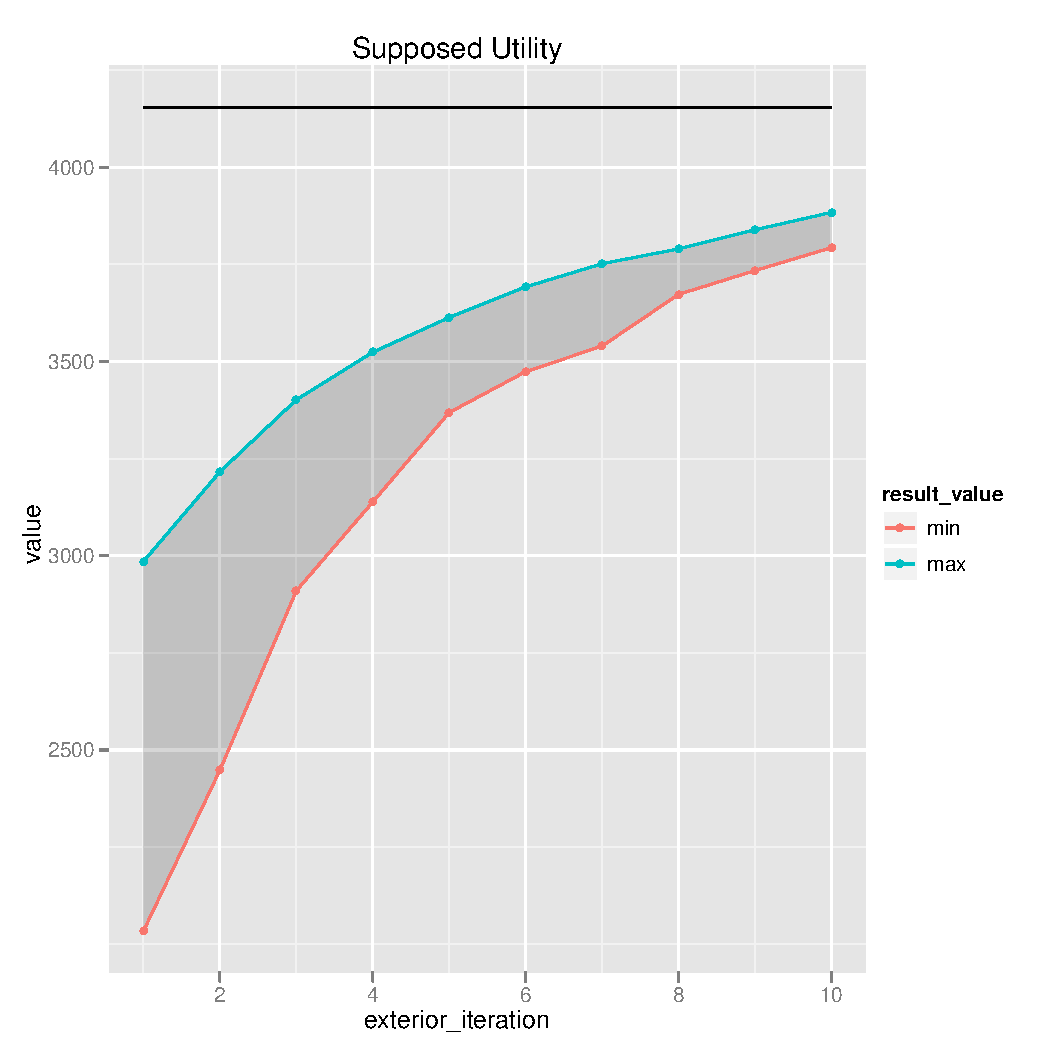
\includegraphics[width=1.0\textwidth]{exp/nouncert/c2_utilouter}
  \caption{Supposed utility function in exterior loop iterations}
  \label{c2_utilouter}
\end{figure}

%% \begin{figure}
%%   \makebox[1\textwidth]{
%%     \subfloat[Subfloat]{
%%       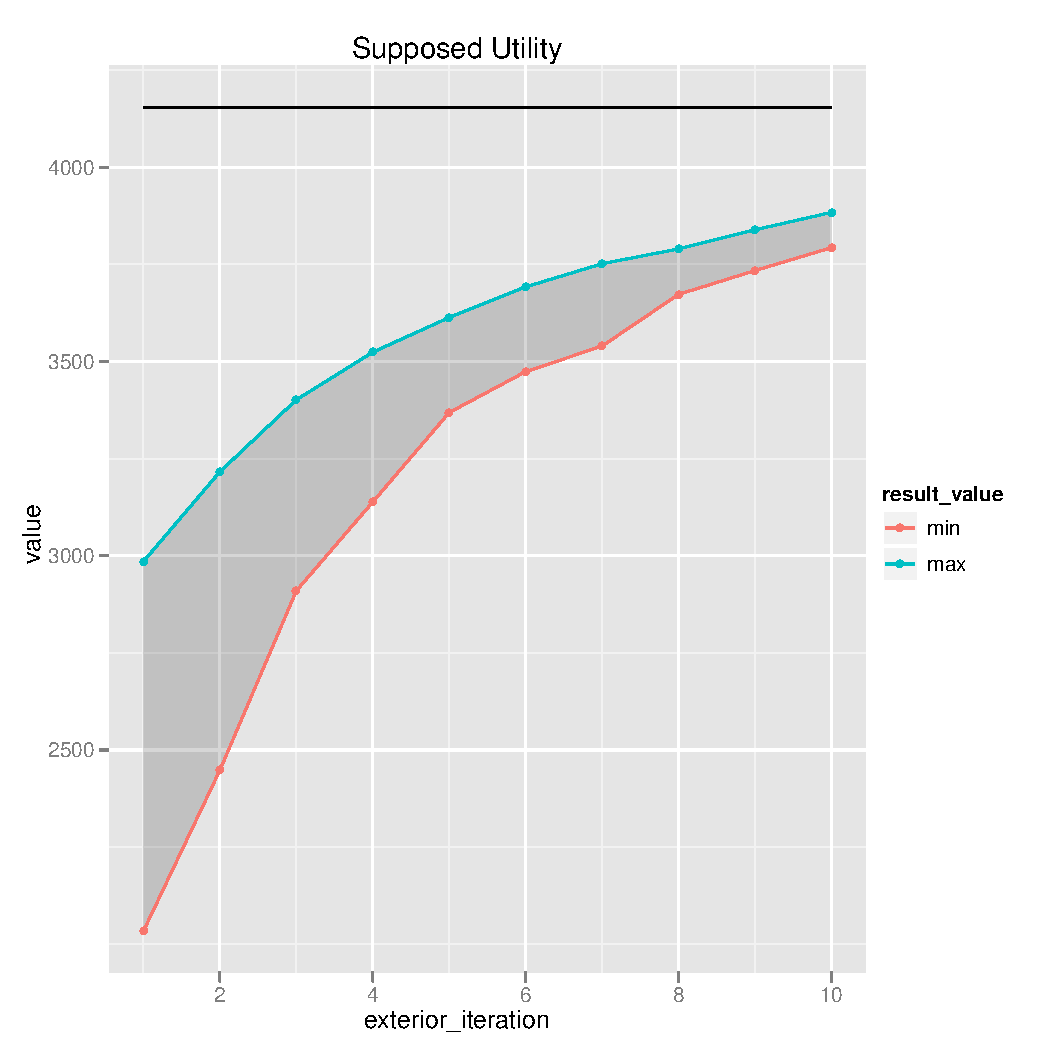
\includegraphics[width=0.6\textwidth]{exp/nouncert/c2_utilouter}
%%     }
%%     \subfloat[Subfloat]{
%%       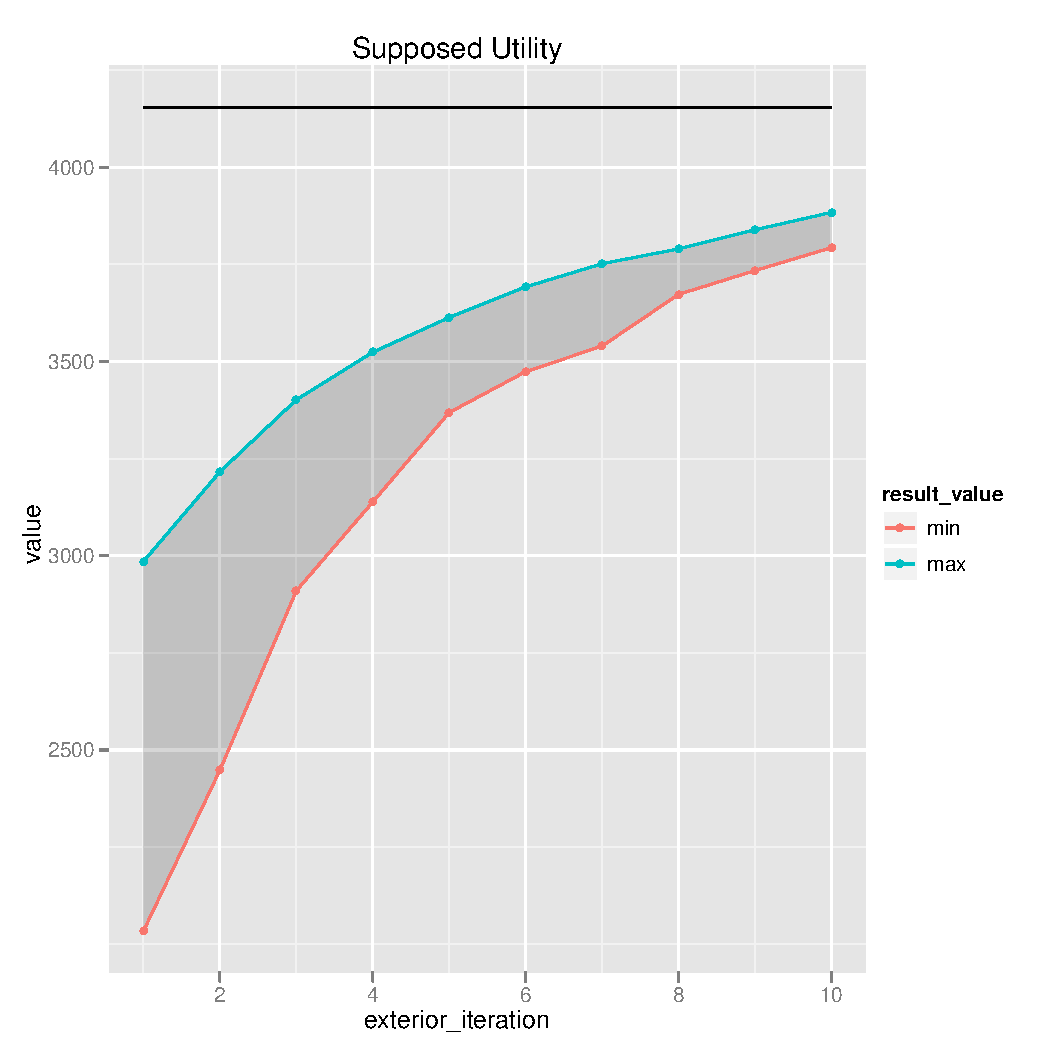
\includegraphics[width=0.6\textwidth]{exp/nouncert/c2_utilouter}
%%     }
%%   }
%%   \caption{Supposed utility function in exterior loop iterations}
%%   \label{c2_utilouter}
%% \end{figure}


%% Utilgen
\begin{figure}
  \centering 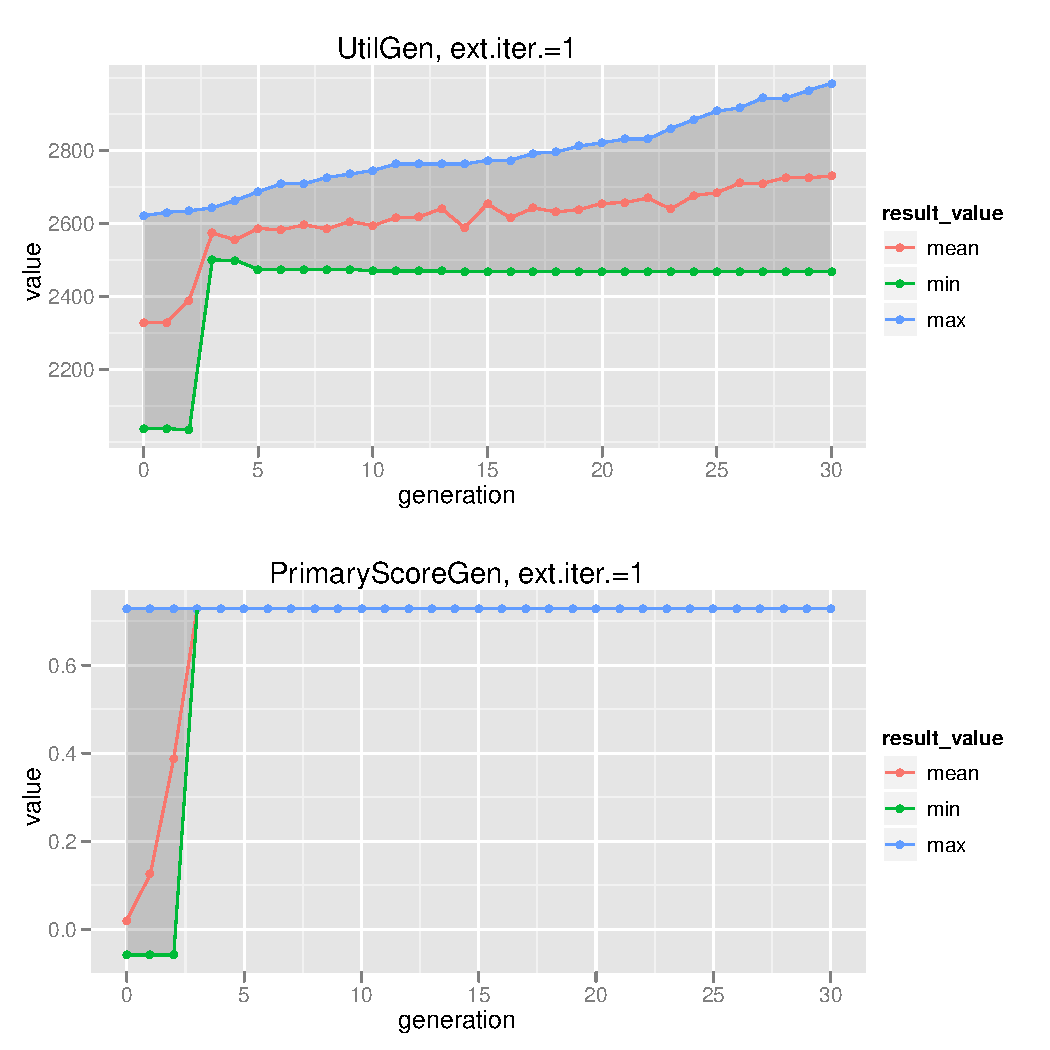
\includegraphics[width=1.0\textwidth]{exp/nouncert/c2_utilgen_01}
  \caption{Supposed utility function in interior loop iterations}
  \label{c2_utilgen_01}
\end{figure}

\begin{figure}
  \centering 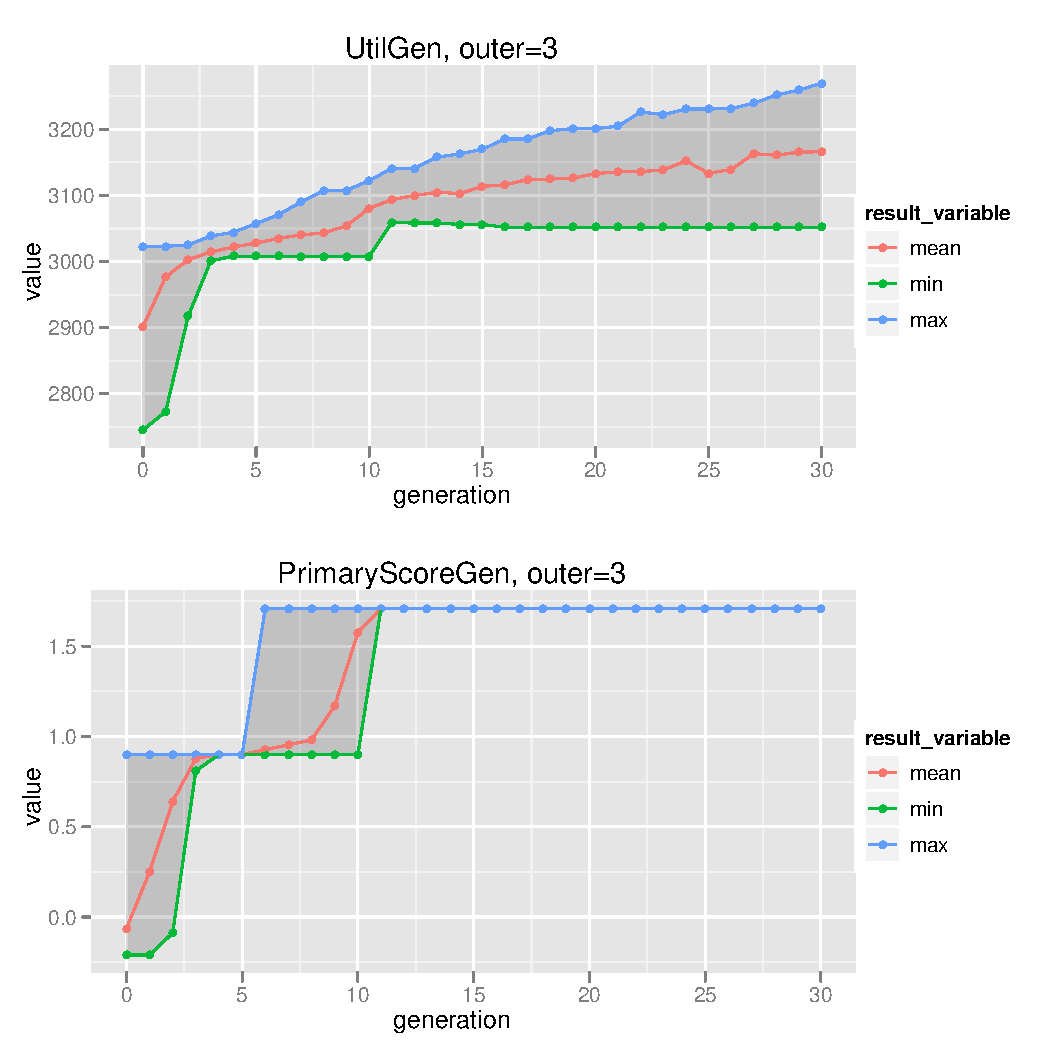
\includegraphics[width=1.0\textwidth]{exp/nouncert/c2_utilgen_03}
  \caption{Supposed utility function in interior loop iterations}
  \label{c2_utilgen_03}
\end{figure}

\begin{figure}
  \centering 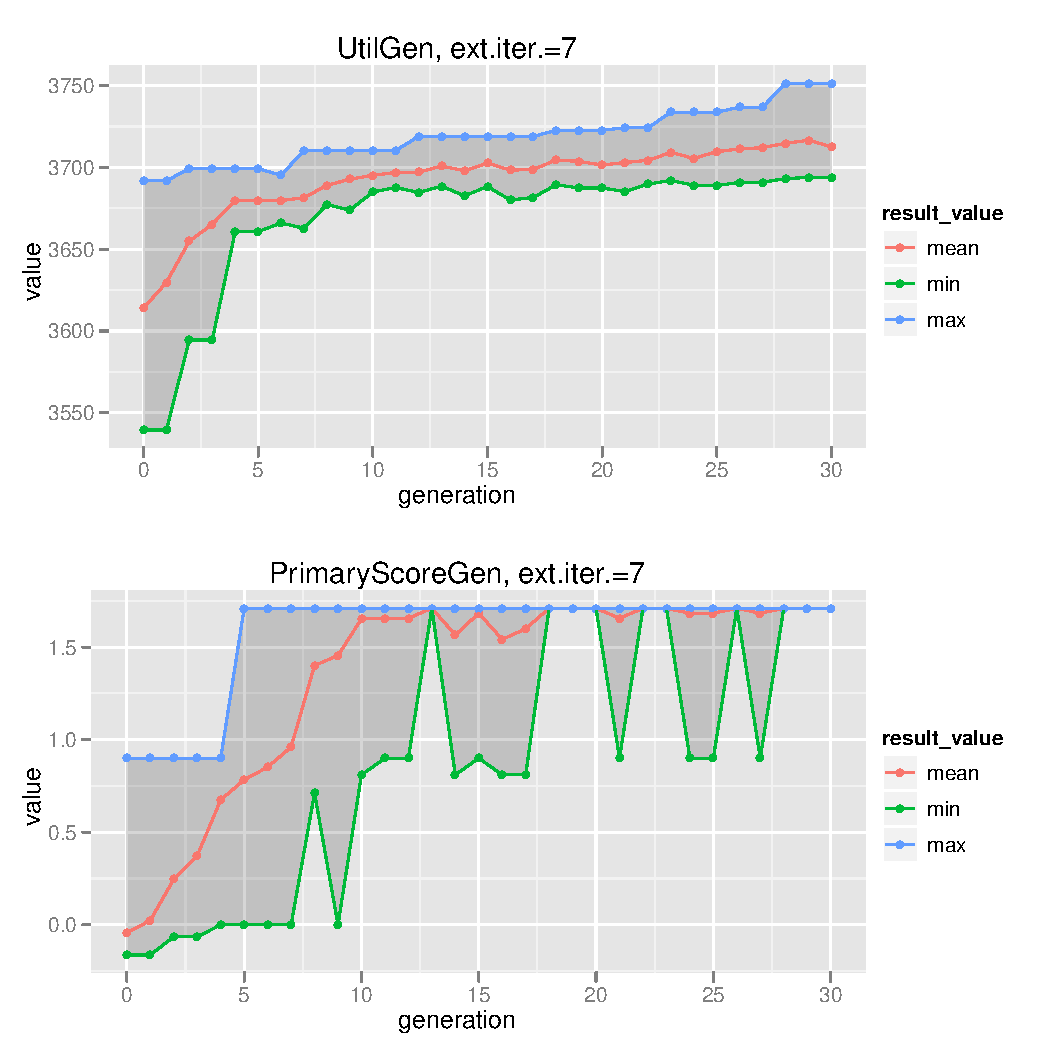
\includegraphics[width=1.0\textwidth]{exp/nouncert/c2_utilgen_07}
  \caption{Supposed utility function in interior loop iterations}
  \label{c2_utilgen_07}
\end{figure}

%% Valweight
\begin{figure}
  \centering
  \makebox[\textwidth]{
    \subfloat{
      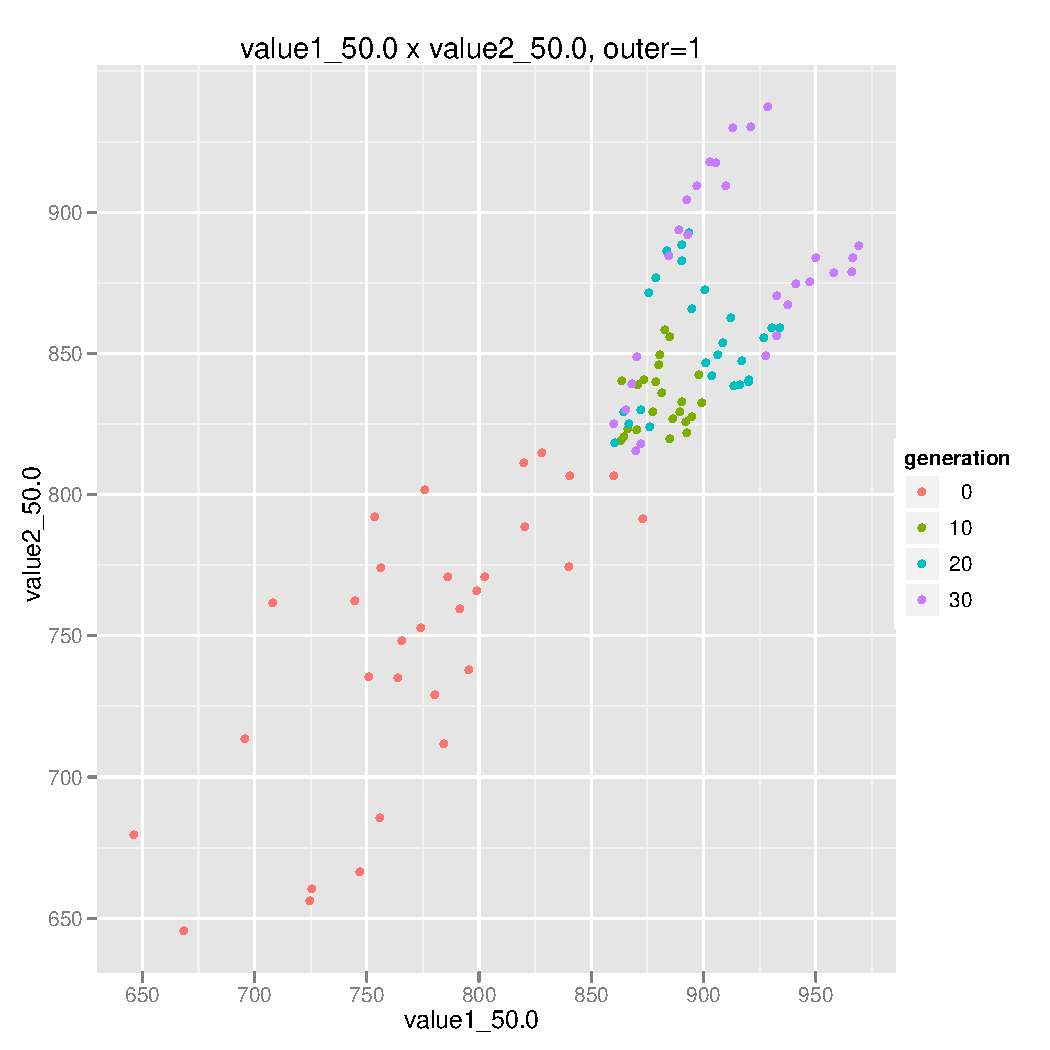
\includegraphics[scale=0.50]{exp/nouncert/c2_valweight_01}
      \label{c2_valweight_01}
    }
    \subfloat{
      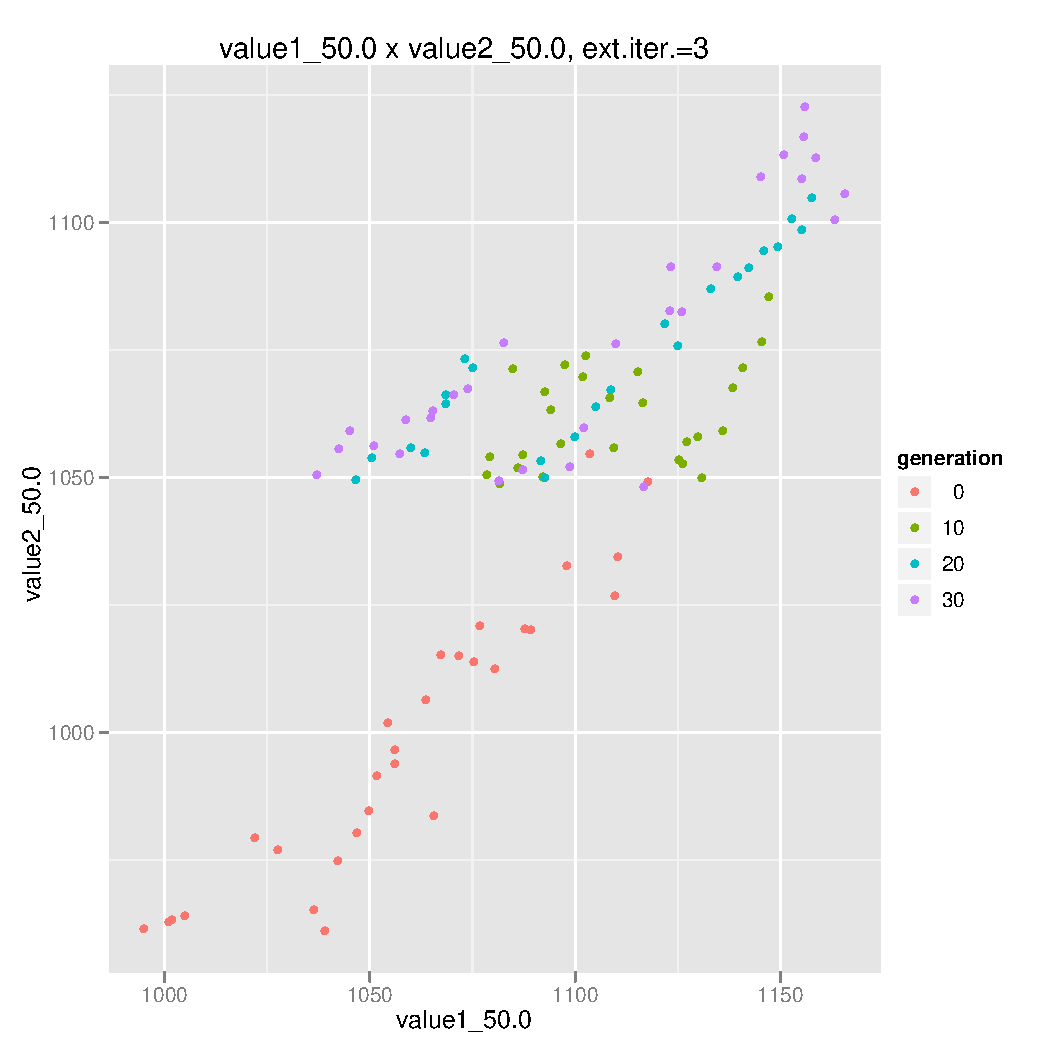
\includegraphics[scale=0.50]{exp/nouncert/c2_valweight_03}
      \label{c2_valweight_03}
    }
  }
  \makebox[\textwidth]{
    \subfloat{
      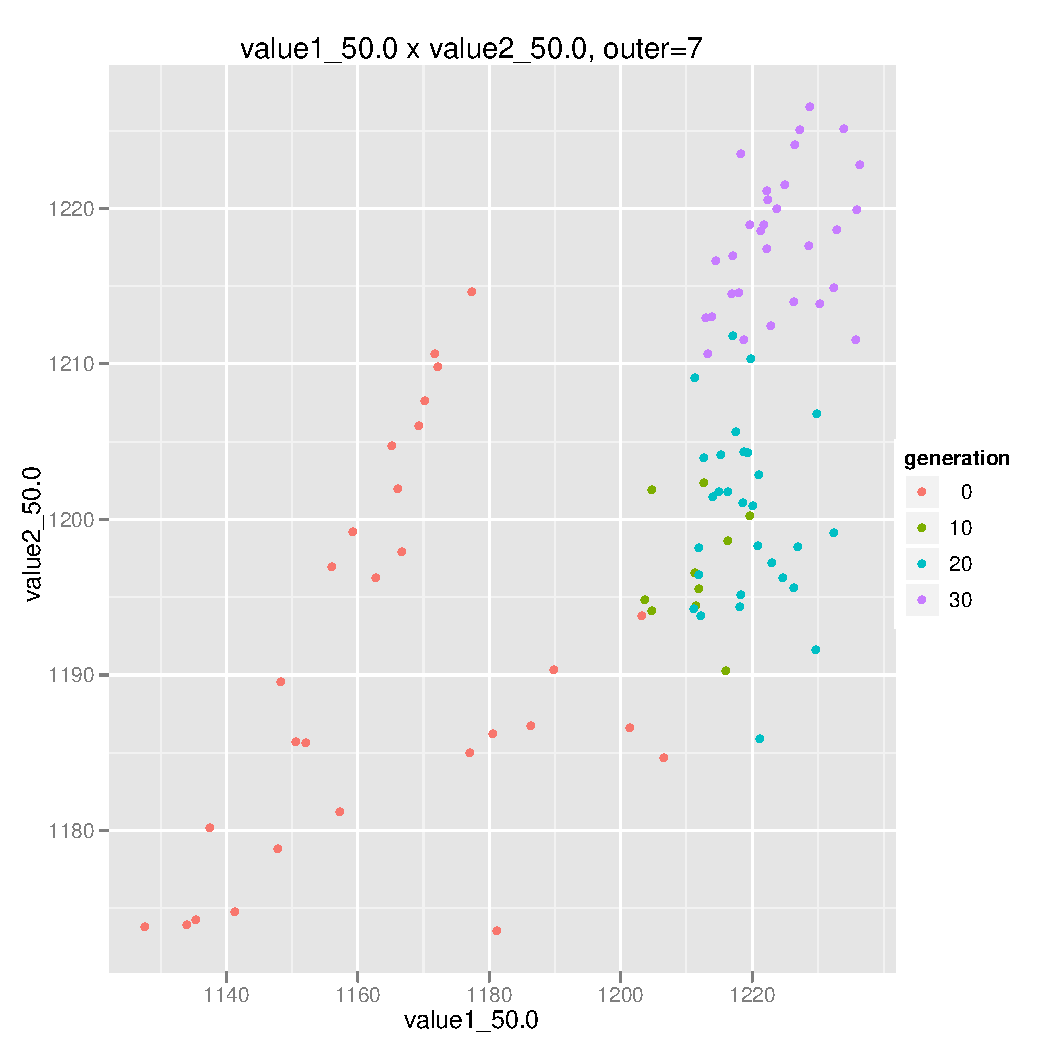
\includegraphics[scale=0.50]{exp/nouncert/c2_valweight_07}
      \label{c2_valweight_07}
    }
  }
  \caption{Individuals in the solution space}
\end{figure}


%% DM's choices
\begin{figure}
  \centering
  \makebox[\textwidth]{
    \subfloat{
      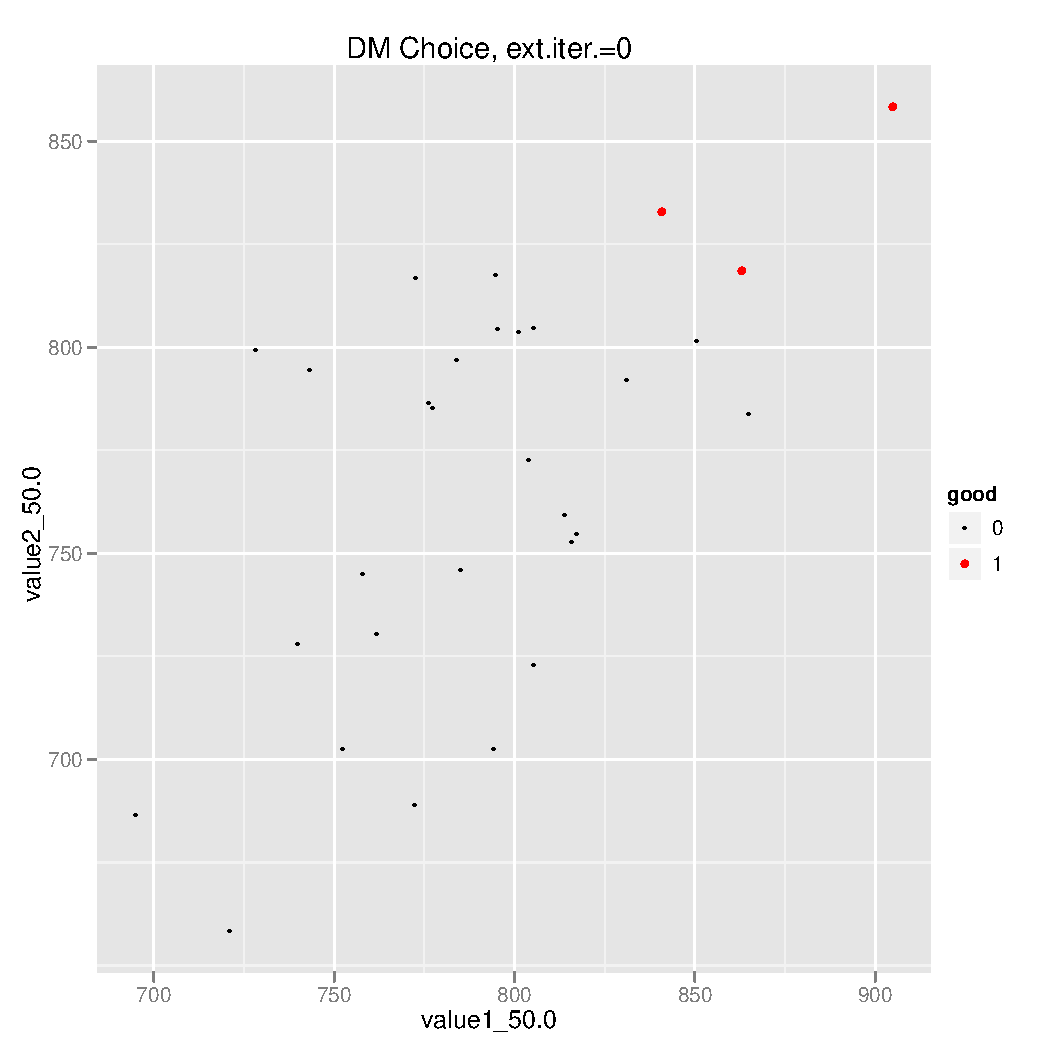
\includegraphics[scale=0.50]{exp/nouncert/c2_dmchoices_01}
      \label{c2_dmchoices_01}
    }
    \subfloat{
      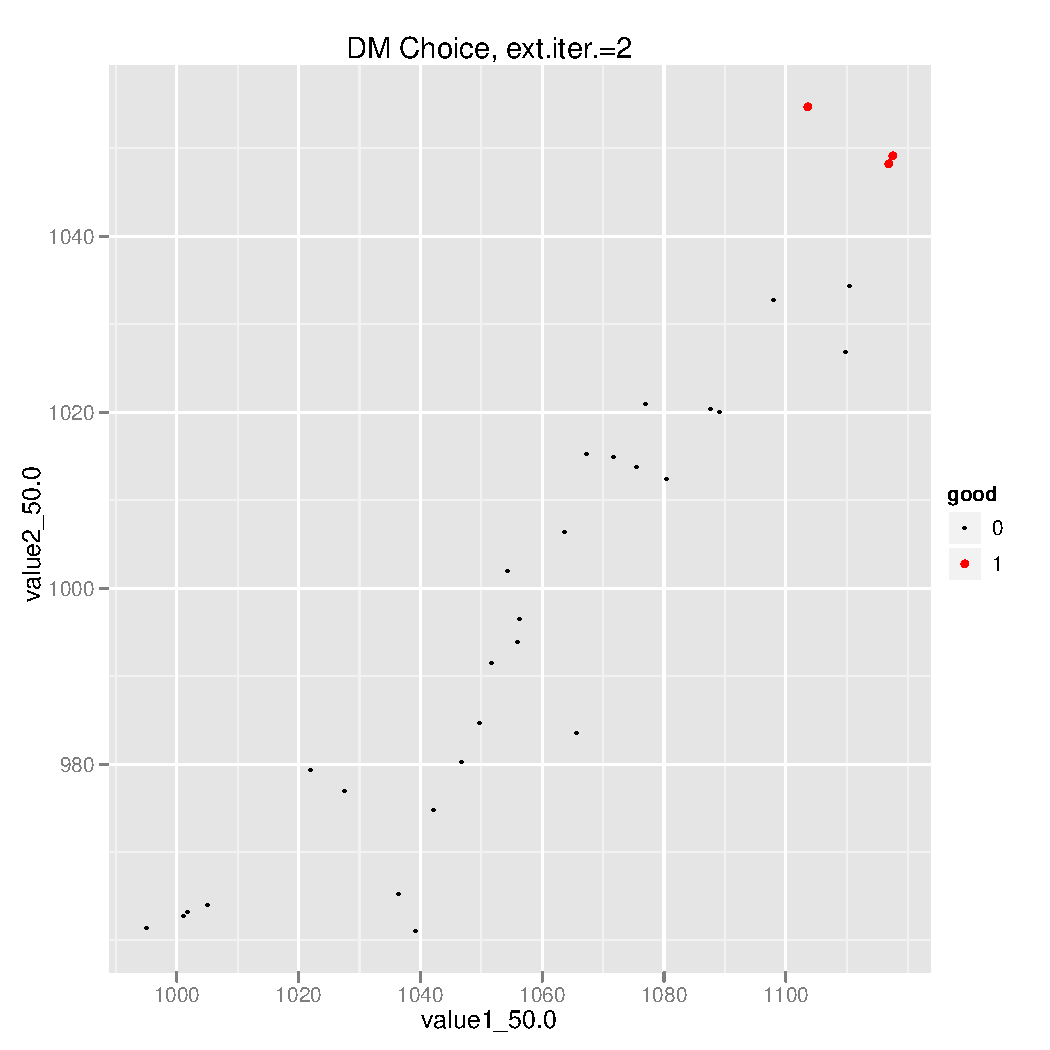
\includegraphics[scale=0.50]{exp/nouncert/c2_dmchoices_03}
      \label{c2_dmchoices_03}
    }
  }
  \makebox[\textwidth]{
    \subfloat{
      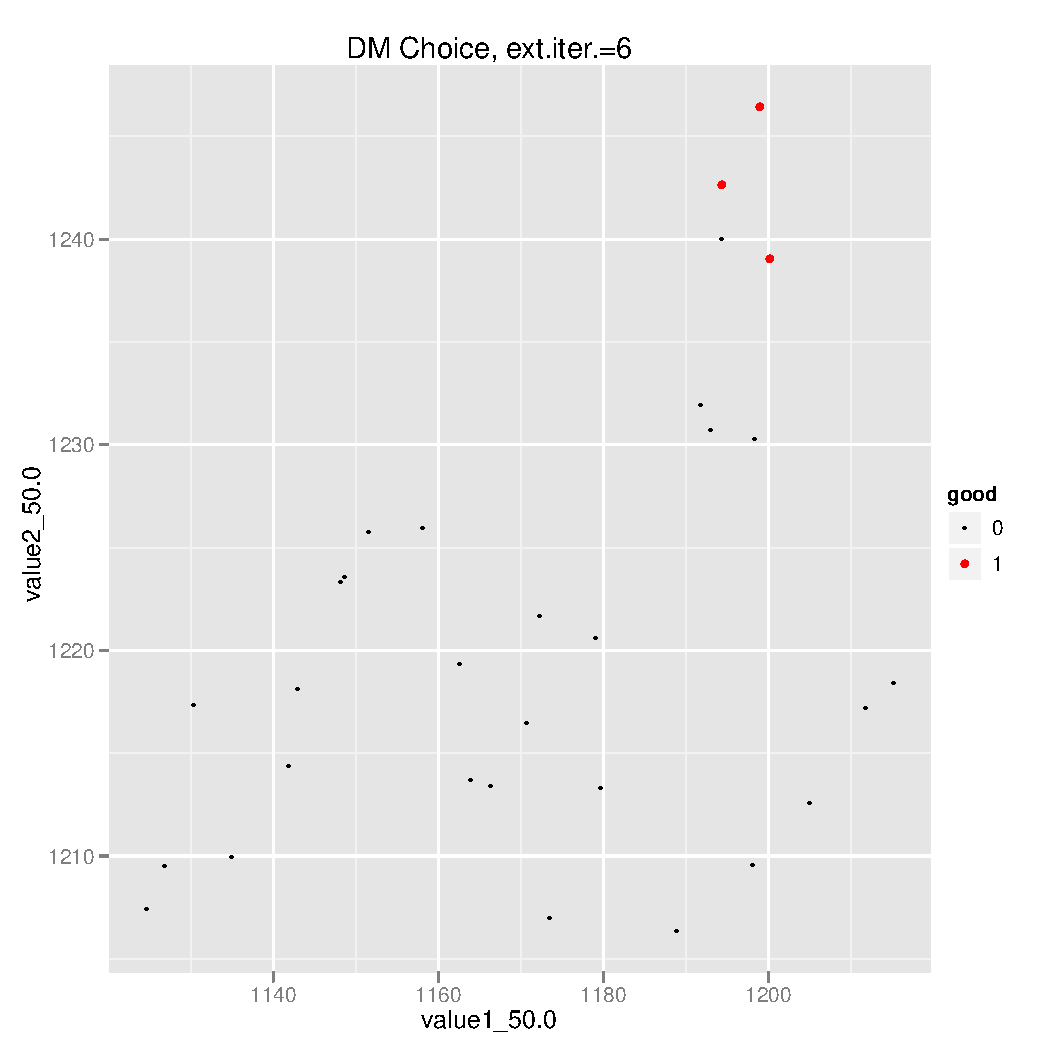
\includegraphics[scale=0.50]{exp/nouncert/c2_dmchoices_07}
      \label{c2_dmchoices_07}
    }
  }
  \caption{Choices made by the DM in exterior loop}
\end{figure}


%% Utilind
\begin{figure}
  \centering 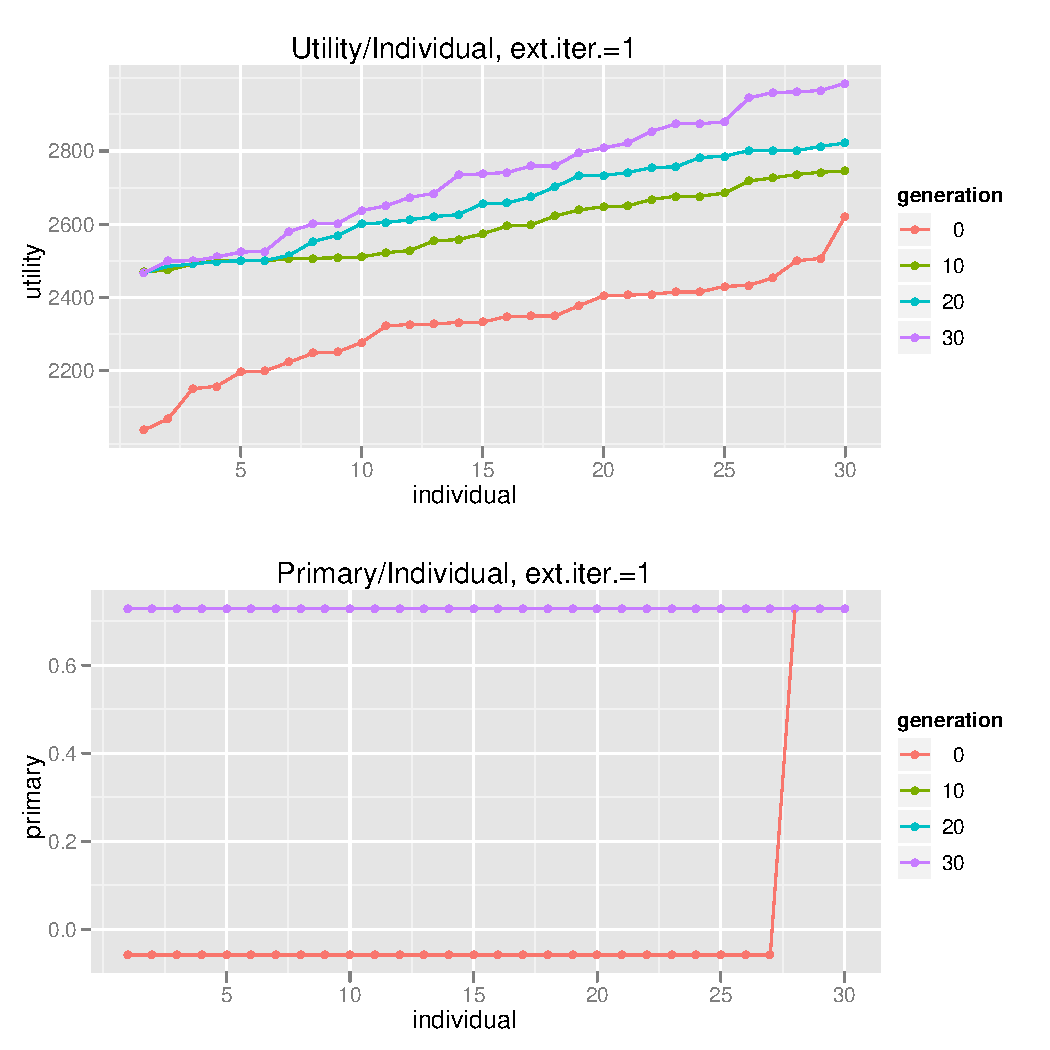
\includegraphics[width=1.0\textwidth]{exp/nouncert/c2_utilind_01}
  \caption{Population advancing through the generations of interior loop}
  \label{c2_utilind_01}
\end{figure}

\begin{figure}
  \centering 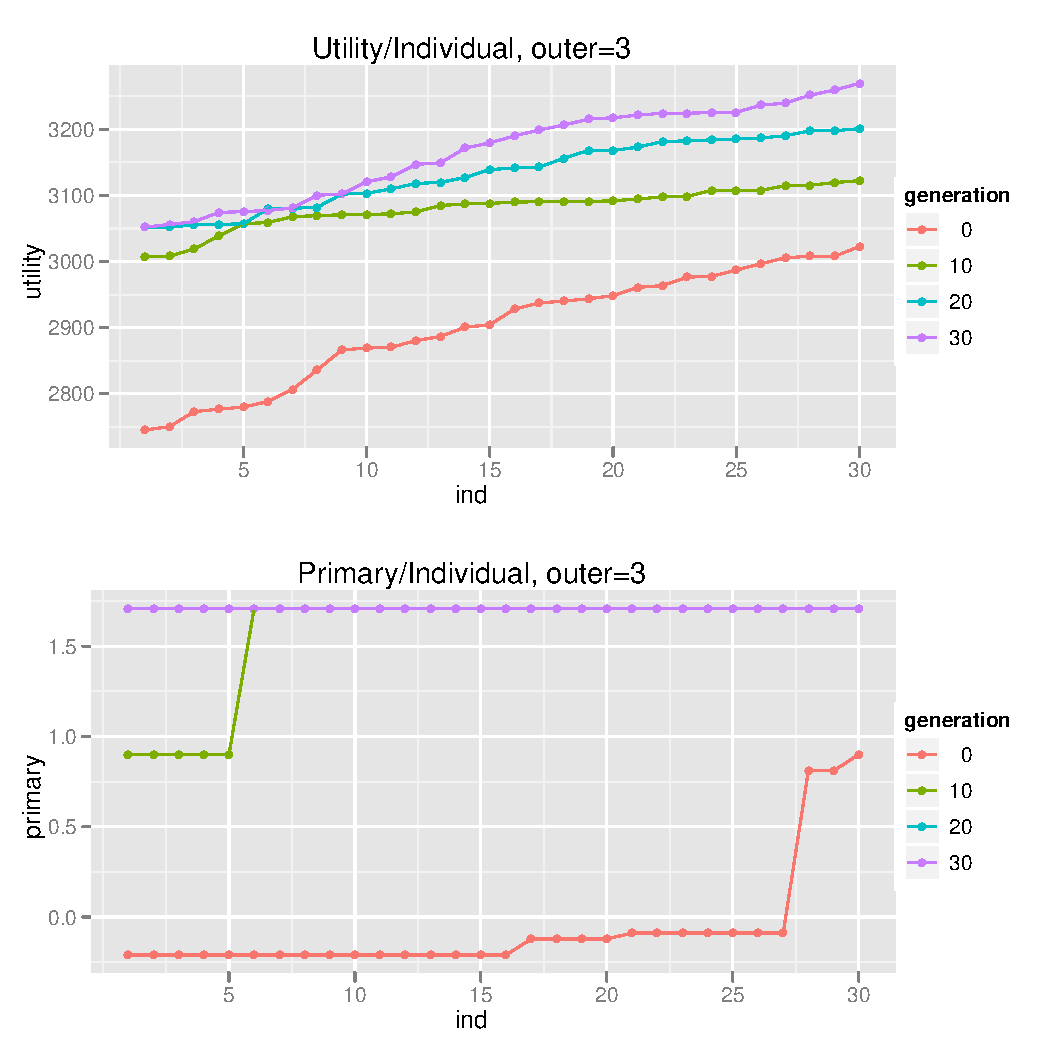
\includegraphics[width=1.0\textwidth]{exp/nouncert/c2_utilind_03}
  \caption{Population advancing through the generations of interior loop}
  \label{c2_utilind_03}
\end{figure}

\begin{figure}
  \centering 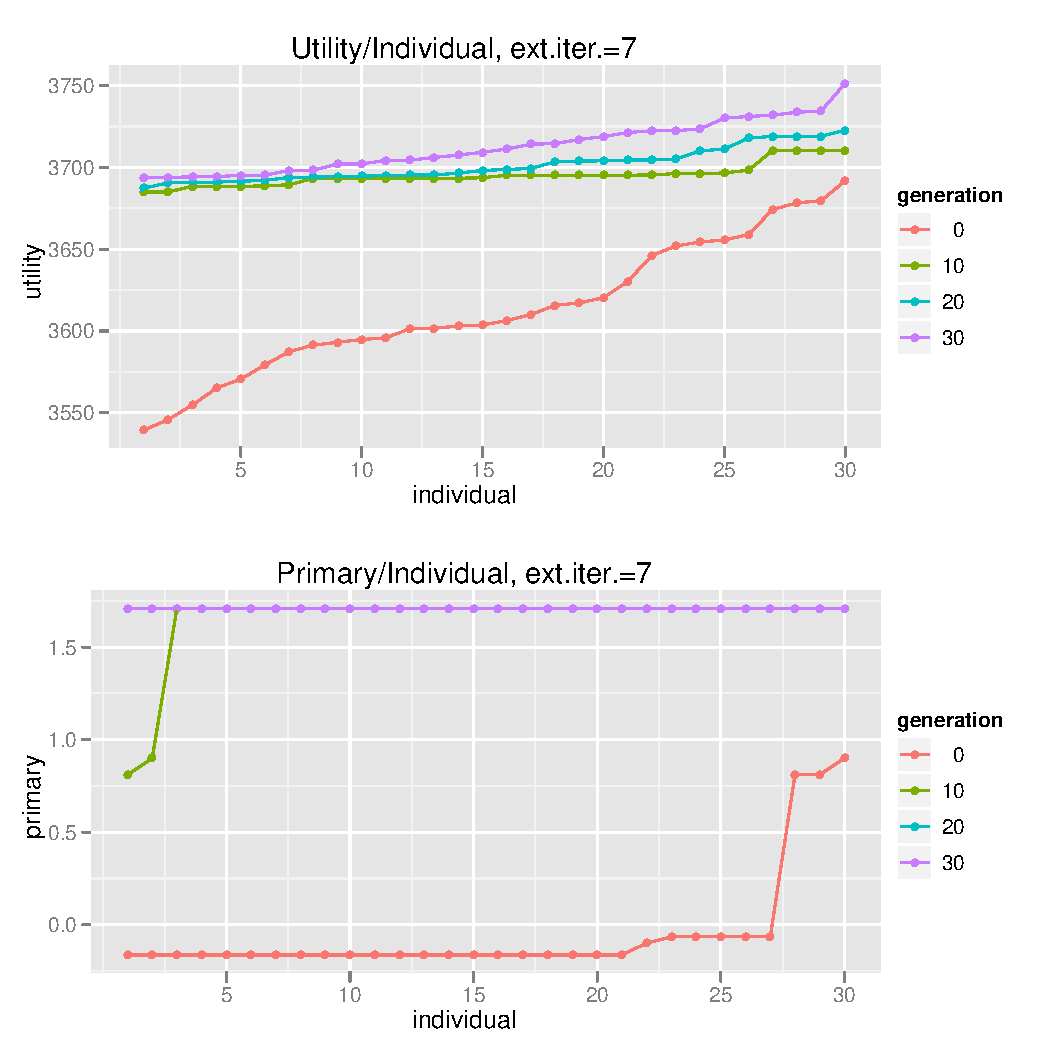
\includegraphics[width=1.0\textwidth]{exp/nouncert/c2_utilind_07}
  \caption{Population advancing through the generations of interior loop}
  \label{c2_utilind_07}
\end{figure}


\clearpage{}
\subsection{The performance on exemplary problems}
\label{nouncert-performance}
It is important to know what performance can be expected from an
algorithm. When no uncertainty is considered in a problem and one assumes
supposed utility function is easy to get optimal solution using linear
programming solver. Of course in real-world applications supposed utility
function is not known a priori. One can test this algorithm in such an
artificially created environment and then assume that the behaviour will be
similar on similar real-world problems.

Results of the evaluation on the following problems are given (see~[inref]):
\begin{itemize}
\item Two-criteria binary knapsack problem, optimal value $= 4154.441453$.
\item Two-criteria continuous knapsack problem, optimal value $= 32700.41689$.
\item Three-criteria binary knapsack problem, optimal value $= 31502.10927$.
\item Three-criteria DTLZ problem generated using constraint surface approach, optimal value $= -1.1$.
\end{itemize}

The test were repeated at least fifteen times and the results averaged. They
are presented on figure~\ref{simple_performance} and
table~\ref{t:opt_dist}. Depending on a problem $10$ or $20$ iterations of
exterior loop were simulated. Normally it would be up to the DM to stop when
he or she is satisfied with the solution. However one can safely assume that
if no satisfactory solution is found in $10$ the decision maker will not want
to investigate the problem with this method further.

\begin{figure}
  \centering
  \makebox[\textwidth]{
    \subfloat{
      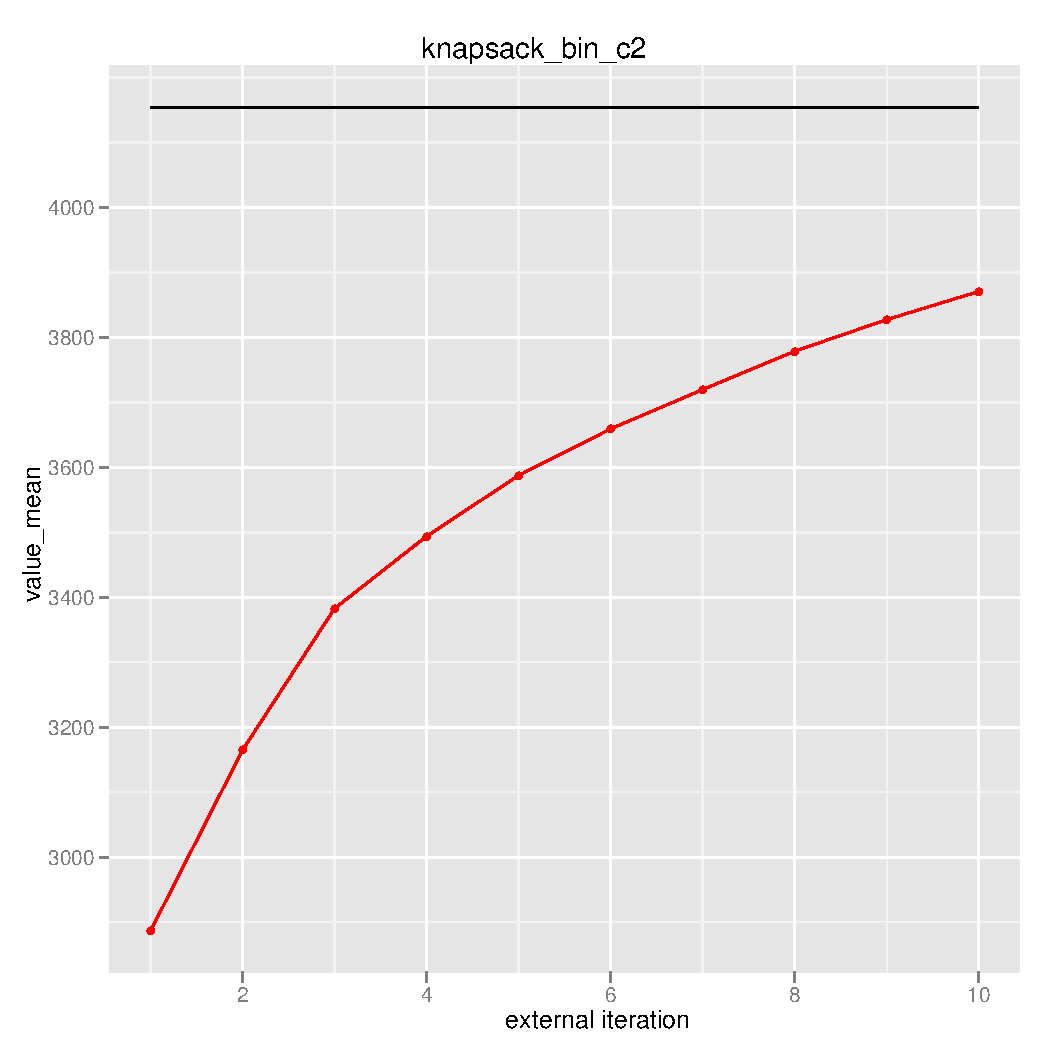
\includegraphics[scale=0.50]{exp/nouncert/c2_knapsack_bin}
      \label{simple_performance1}
    }
    \subfloat{
      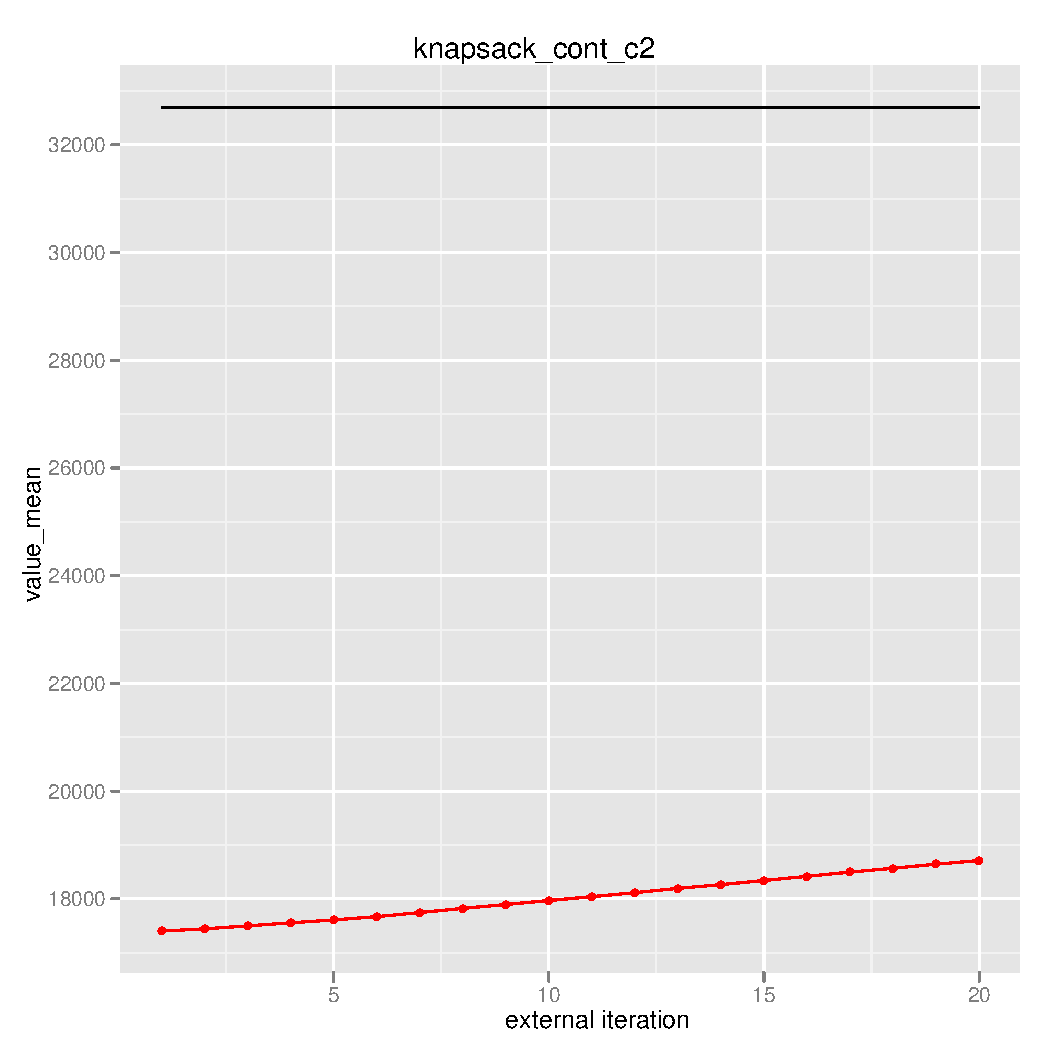
\includegraphics[scale=0.50]{exp/nouncert/c2_knapsack_cont}
      \label{simple_performance2}
    }
  }
  \makebox[\textwidth]{
    \subfloat{
      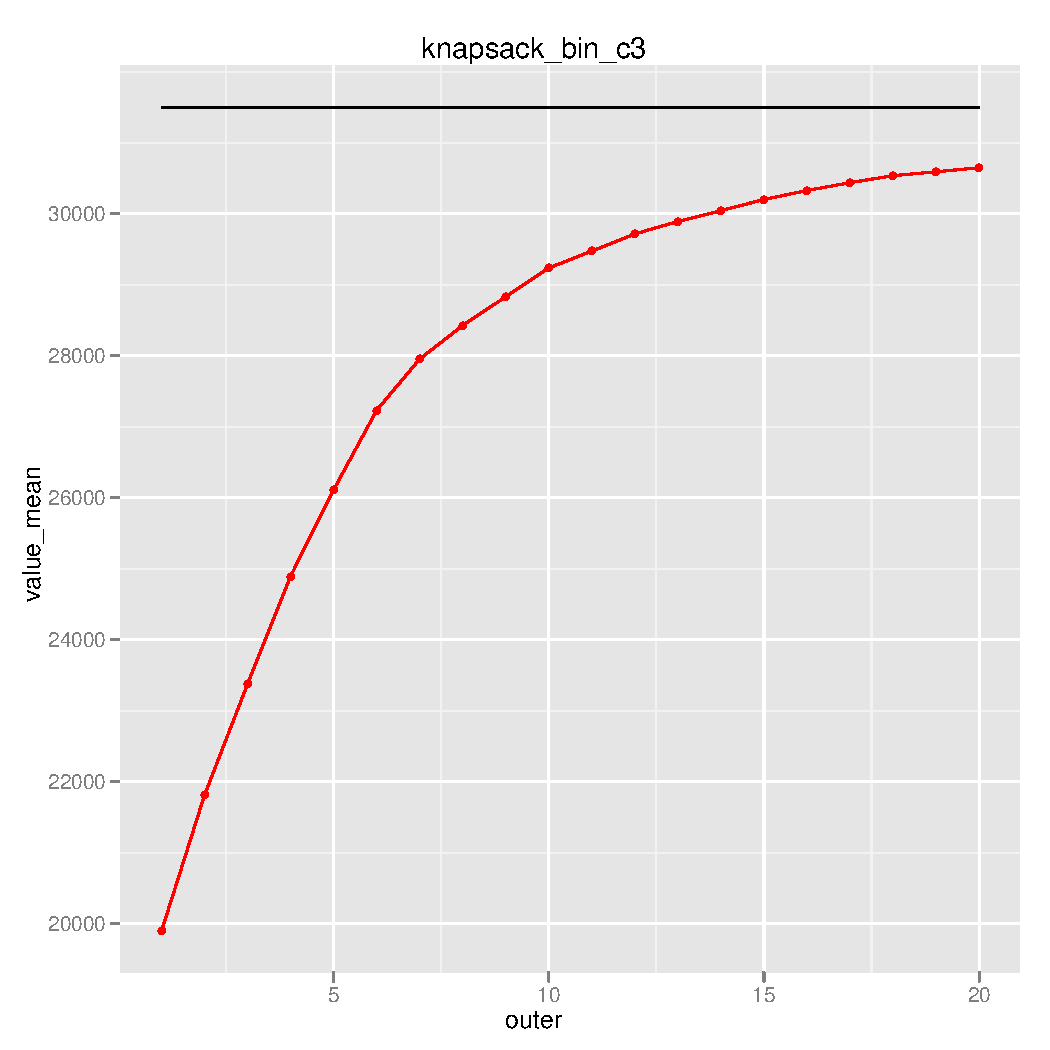
\includegraphics[scale=0.50]{exp/nouncert/c3_knapsack_bin}
      \label{simple_performance3}
    }
    \subfloat{
      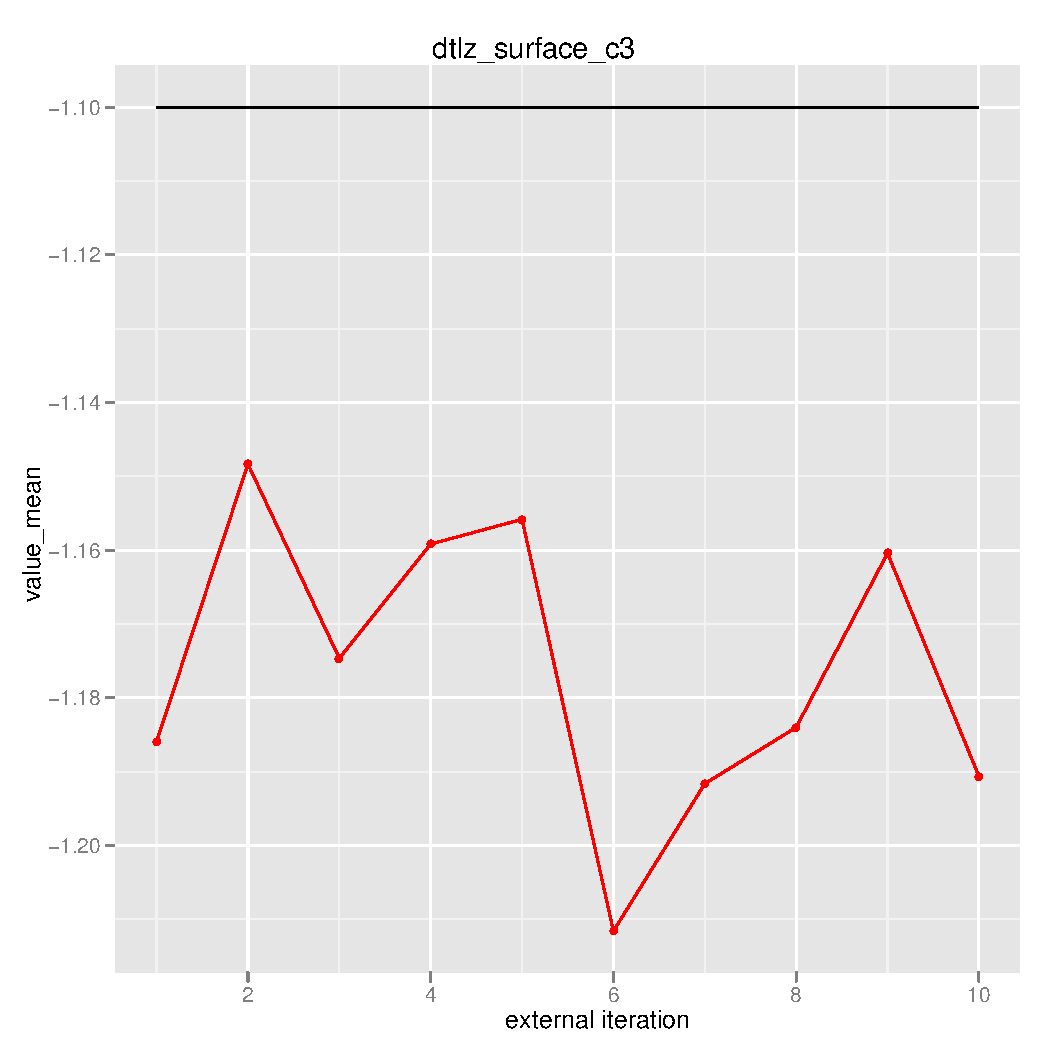
\includegraphics[scale=0.50]{exp/nouncert/c3_surface}
      \label{simple_performance4}
    }
  }
  \caption{Performance comparison}
  \label{simple_performance}
\end{figure}

\begin{table}
  \centering
  \caption{Distance from the optimum solution}
  \label{t:opt_dist}
  \begin{tabular}{r c c c c}
    \hline
    Exterior loop & Knapsack bin 2c & Knapsack cont 2c & Knapsack bin 3c &
    DTLZ surface 3c \\
    \hline
    \hline
    1. & 30.52\% & 46.79\% & 36.85\% & 7.82\% \\
    2. & 23.84\% & 46.66\% & 30.77\% & 4.40\% \\
    3. & 18.61\% & 46.49\% & 25.80\% & 6.79\% \\
    4. & 15.96\% & 46.32\% & 20.99\% & 5.38\% \\
    5. & 13.73\% & 46.16\% & 17.12\% & 5.08\% \\
    6. & 12.02\% & 45.97\% & 13.57\% & 10.15\% \\
    7. & 10.59\% & 45.74\% & 11.28\% & 8.33\% \\
    8. & 9.20\% & 45.51\% & 9.78\% & 7.64\% \\
    9. & 8.05\% & 45.29\% & 8.50\% & 5.49\% \\
    10. & 7.03\% & 45.06\% & 7.22\% & 8.24\% \\
    11. & - & 44.85\% & 6.47\% & - \\
    12. & - & 44.62\% & 5.70\% & - \\
    13. & - & 44.38\% & 5.15\% & - \\
    14. & - & 44.17\% & 4.67\% & - \\
    15. & - & 43.94\% & 4.17\% & - \\
    16. & - & 43.70\% & 3.77\% & - \\
    17. & - & 43.46\% & 3.43\% & - \\
    18. & - & 43.25\% & 3.12\% & - \\
    19. & - & 43.02\% & 2.94\% & - \\
    20. & - & 42.81\% & 2.77\% & - \\
    \hline
  \end{tabular}
\end{table}

On both binary knapsack problems the performance is very good --- they are not
further than $10\%$ away from optimal solution after $10^{th}$ iteration. The
same is true for the surface problem. However looking at the
fig.~\ref{simple_performance4} one can see a bizarre phenomenon --- the
supposed utility is falling down in a few runs.

On the other hand evolutionary algorithm knows nothing about the utility
function so it may happen. The chart (fig.~\ref{simple_performance4}) was
generated using aggregated (averaged) results, however this happened in most
of the runs. To give further insight charts showing evolution in a third
exterior loop are presented (not that the charts are for single run only, not
aggregated). The charts are on figures~\ref{c3_surface_utilgen_03}
and~\ref{c3_surface_utilind_03}. As one can see the evolutionary algorithm
improves the population from its perspective (the primary score factor)
however supposed utility function is being lowered in the process.

\begin{figure}
  \centering
  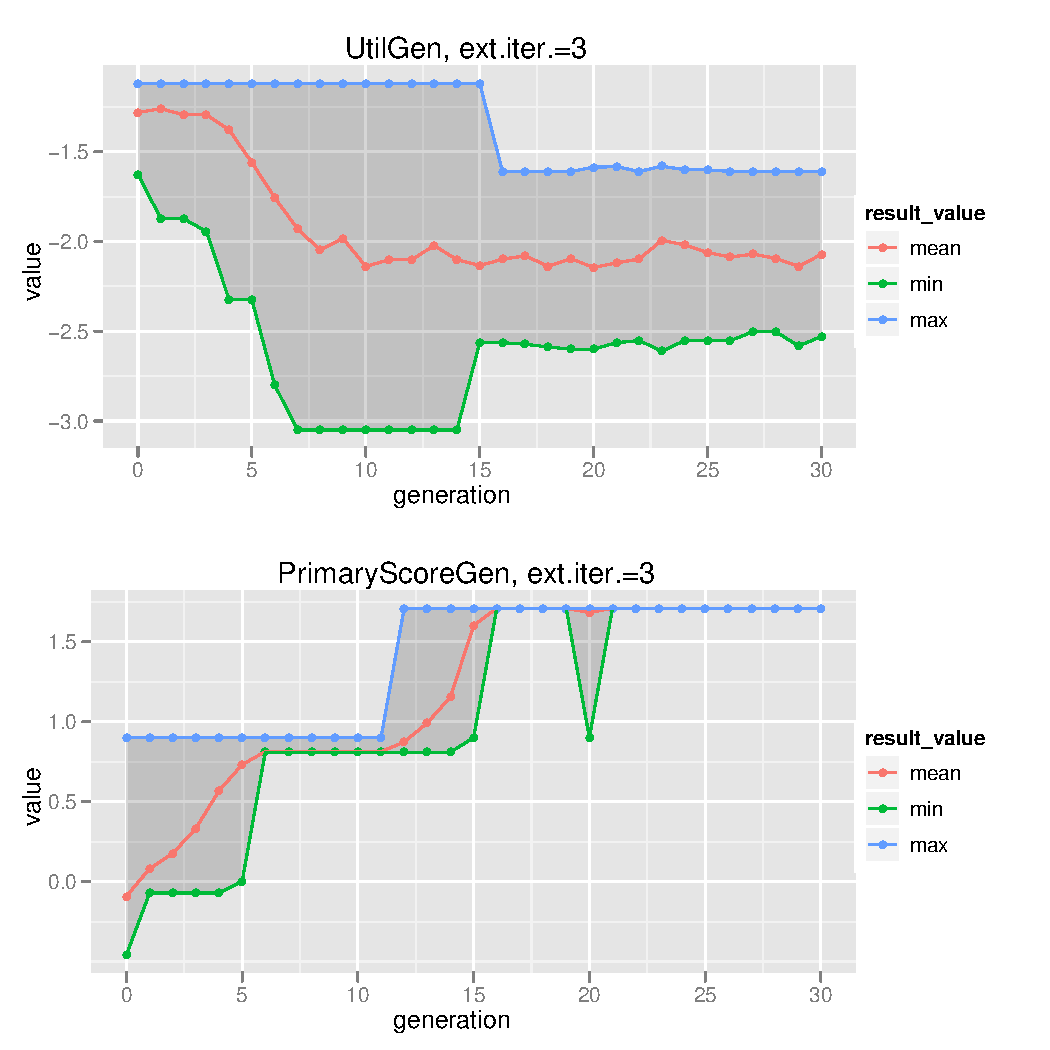
\includegraphics[width=1.0\textwidth]{exp/nouncert/c3_surface_utilgen_03}
  \caption{The population in the third iteration of the exterior loop. DTLZ
    surface problem.}
  \label{c3_surface_utilgen_03}
\end{figure}

\begin{figure}
  \centering
  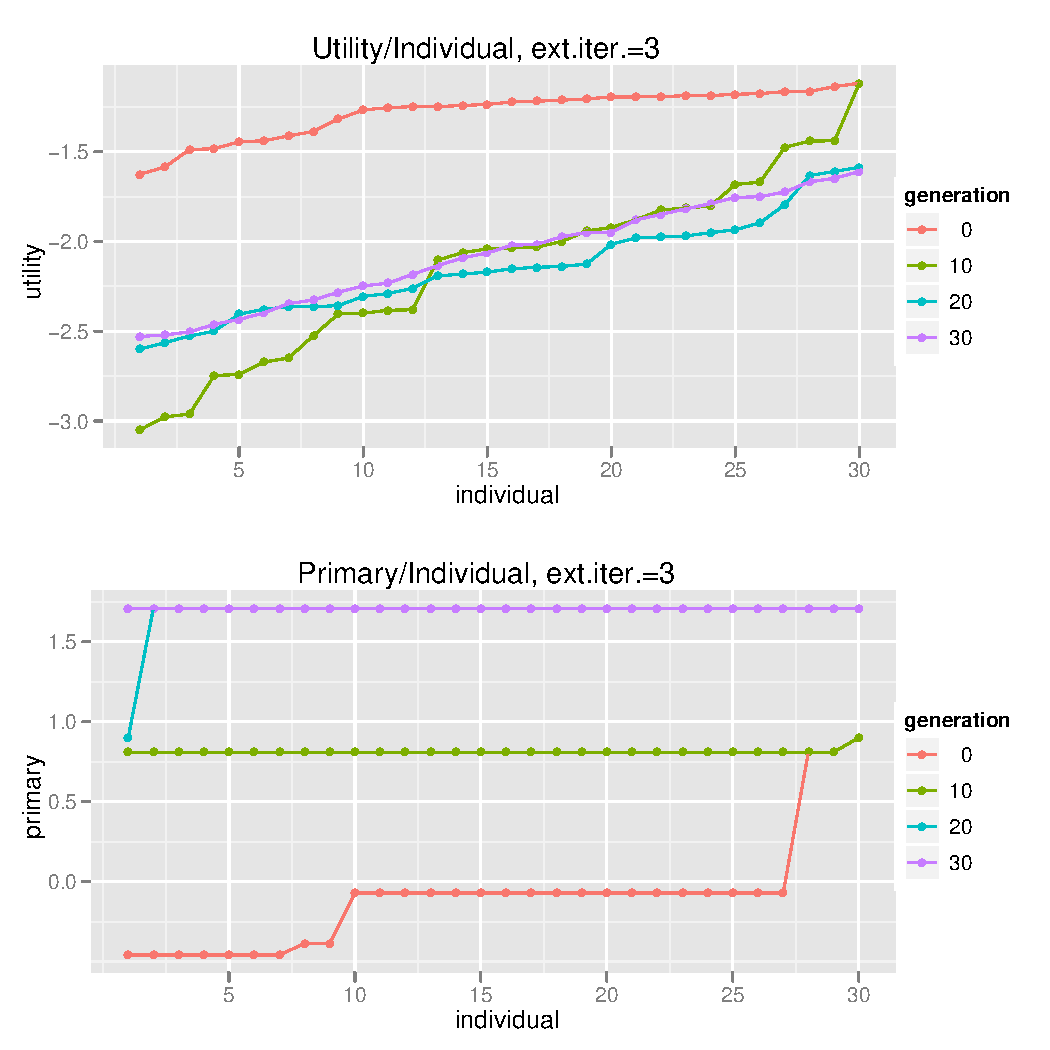
\includegraphics[width=1.0\textwidth]{exp/nouncert/c3_surface_utilind_03}
  \caption{The population in the third iteration of the exterior loop. DTLZ
    surface problem}
  \label{c3_surface_utilind_03}
\end{figure}

This is the case because generated decision rules:
\begin{enumerate}
\item $f_1 \le 0.14033 \Rightarrow \text{class} \ge \texttt{GOOD}$
\item $f_3 \le 0.56462 \Rightarrow \text{class} \ge \texttt{GOOD}$
\end{enumerate}
are not selective enough. It is possible than switching DomLem to another
algorithm, generating all possible rules instead of minimal set would help
here. Still the results achieved by the DARWIN method are good on this
problem.

In contrary continuous knapsack problem performs extremely poor --- only
$55\%$ of the optimum after $10^{th}$ run and $58\%$, so almost no
improvement, after $20^{th}$. Investigating single runs in details provided no
more details. The problem lies in the evolutionary algorithm, more precisely
in its crossover operator. Authors suggested a from of distance preserving
crossover --- child is somewhere in between its parents. However in continuous
it is usually the case to take items one-by-one starting with the one with
greatest value per unit until the weight constraint is reached.

Considering the constraints ($ \forall_{x_i \in items}: \hspace{0.1cm} 0 \leq
x_i \leq 1 $) --- most of the individuals will have its decision variables in
form of $x_i \approx 0.5$ after a few generations. But for the optimal
solutions most of the variables takes either $1$ or $0$. That is why
improvement is happening so slowly here.

According to authors intuition changing the crossover operator would solve the
problem with continuous knapsack. Choosing the right operator for a given
problem is a well-known subject in the multi-objective optimisation
([ref]). However it is out-of-scope of this paper.

For completeness charts presenting the algorithm behaviour when more exterior
loop iterations are allowed are given (fig.~\ref{outer},
table~\ref{t:opt_dist_long}). After the twentieth loop improvements are small
(if any). In author's opinion this is a good thing because there is no reason
not to stop algorithm. If it works for the problem it will be evident from the
first few iterations.

\begin{figure}
  \centering
  \makebox[\textwidth]{
    \subfloat{
      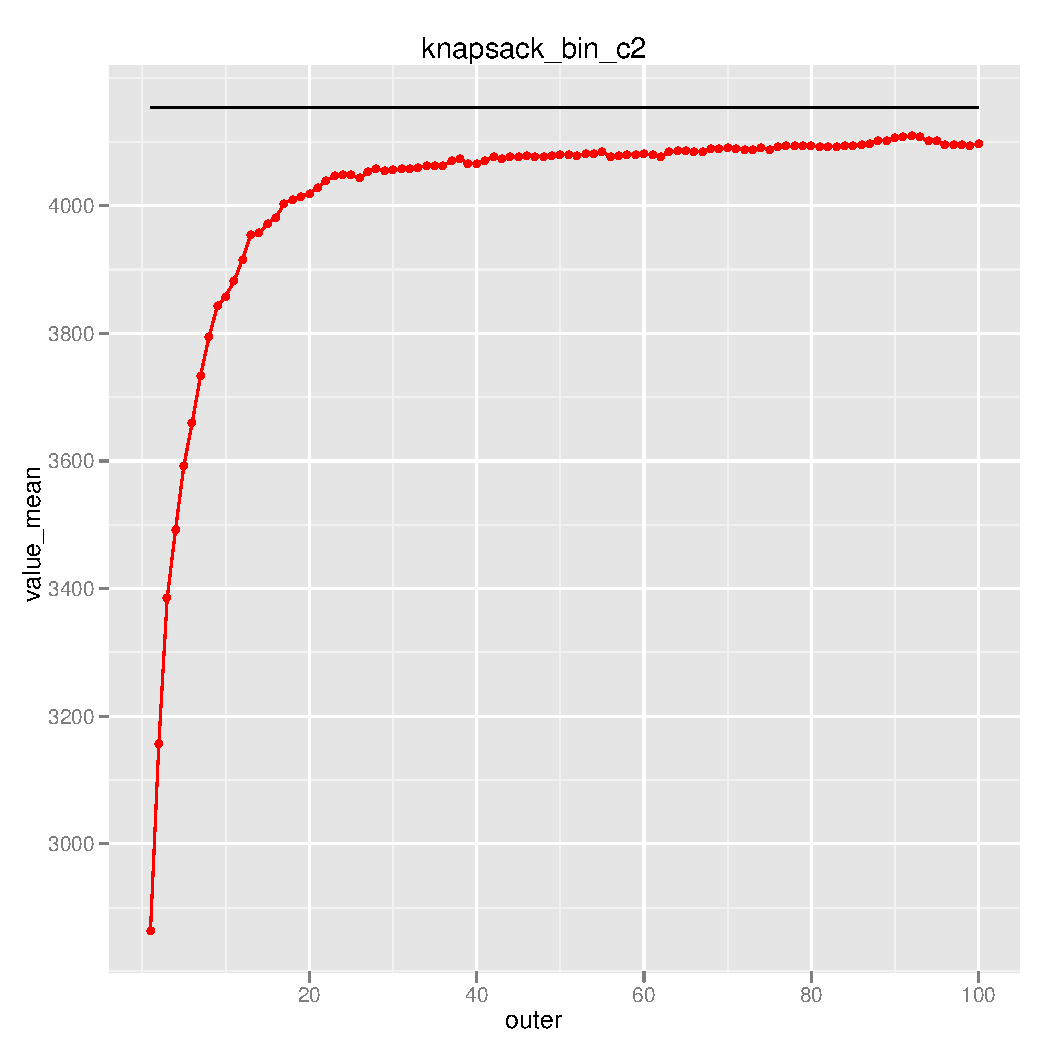
\includegraphics[scale=0.50]{exp/nouncert/c2_knapsack_bin_outer}
      \label{outer1}
    }
    \subfloat[TODO!]{
      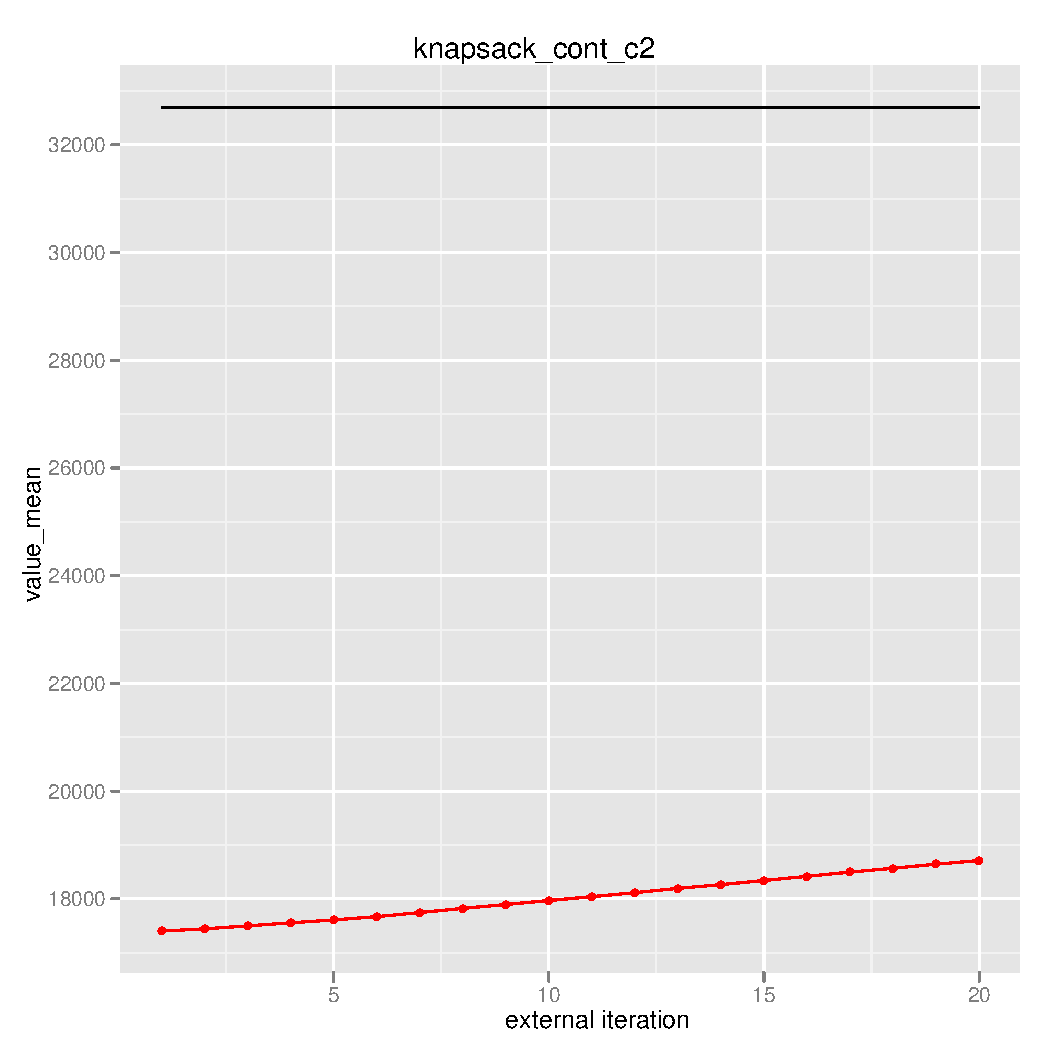
\includegraphics[scale=0.50]{exp/nouncert/c2_knapsack_cont}
      \label{outer2}
    }
  }
  \makebox[\textwidth]{
    \subfloat{
      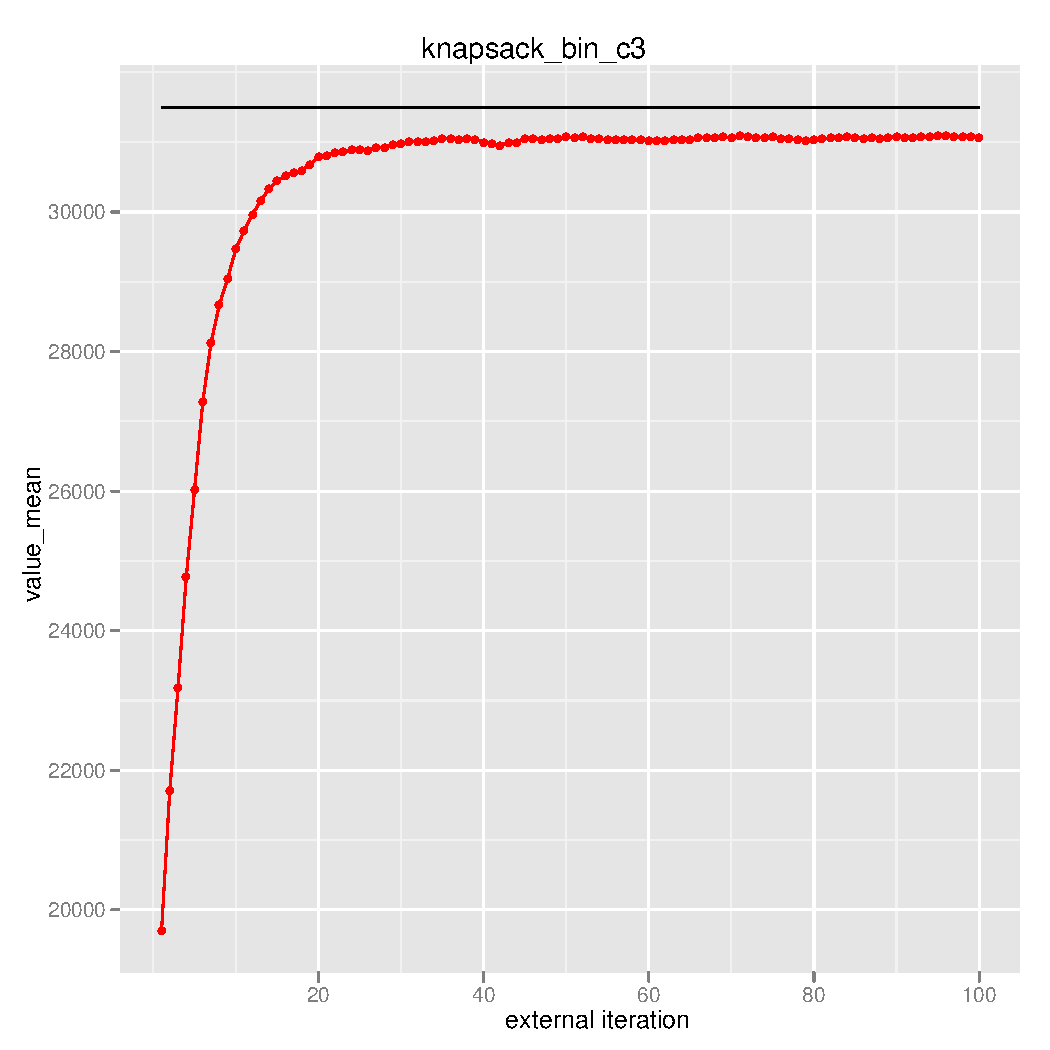
\includegraphics[scale=0.50]{exp/nouncert/c3_knapsack_bin_outer}
      \label{outer3}
    }
    \subfloat{
      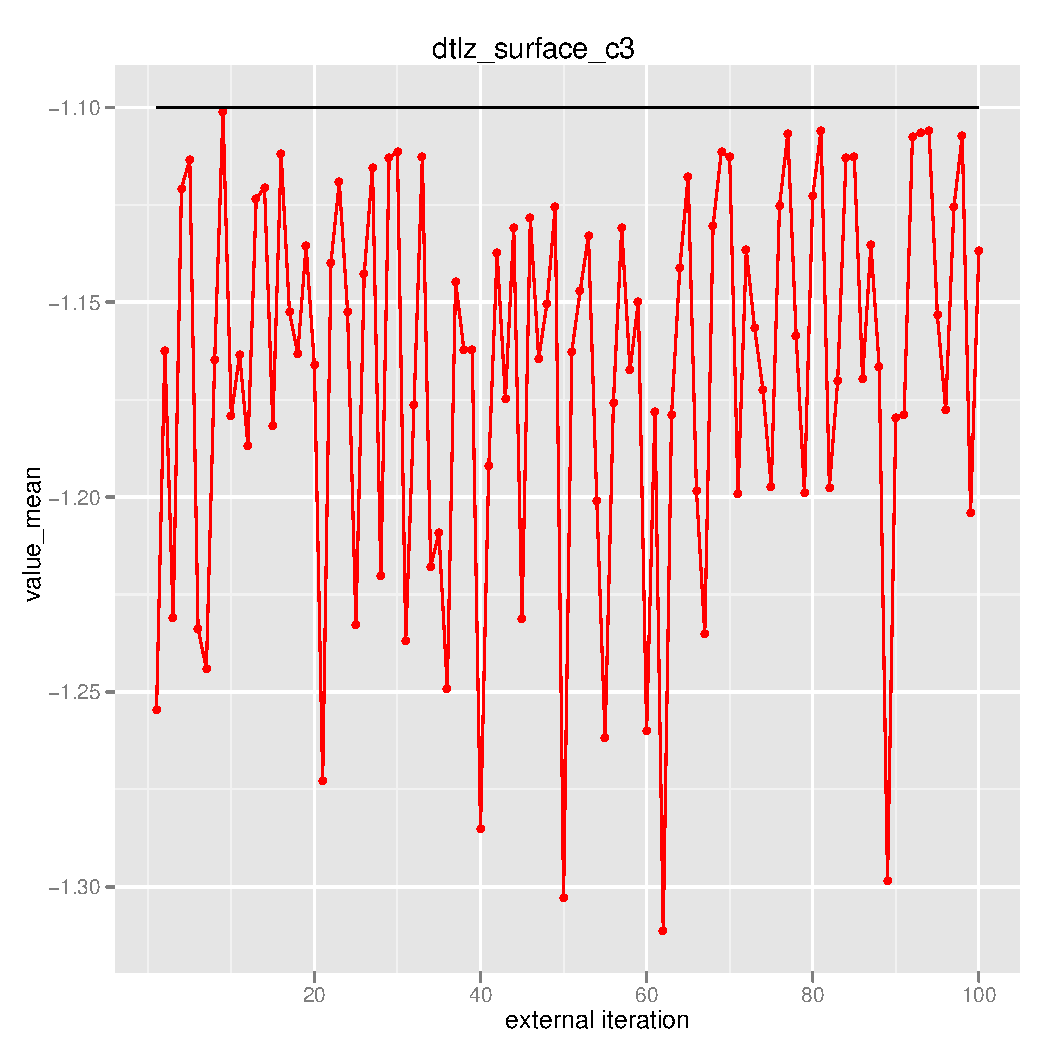
\includegraphics[scale=0.50]{exp/nouncert/c3_surface_outer}
      \label{outer4}
    }
  }
  \caption{Supposed utility function when long runs are allowed}
  \label{outer}
\end{figure}

\begin{table}
  \centering
  \caption{Distance from the optimum solution when long runs are allowed}
  \label{t:opt_dist_long}
  \begin{tabular}{r c c c c}
    \hline
    Exterior loop & Knapsack bin 2c & Knapsack cont 2c & Knapsack bin 3c &
    DTLZ surface 3c \\
    \hline
    \hline
    1 & 31.08\% & TODO & 37.48\% & 14.05\% \\
    5 & 13.59\% & TODO & 17.42\% & 1.22\% \\
    10 & 7.33\% & TODO & 6.48\% & 7.19\% \\
    15 & 4.72\% & TODO & 3.39\% & 7.43\% \\
    20 & 3.70\% & TODO & 2.33\% & 6.00\% \\
    25 & 3.11\% & TODO & 2.02\% & 12.06\% \\
    30 & 3.05\% & TODO & 1.75\% & 1.05\% \\
    35 & 2.99\% & TODO & 1.56\% & 9.93\% \\
    40 & 3.05\% & TODO & 1.73\% & 16.83\% \\
    45 & 2.91\% & TODO & 1.58\% & 11.93\% \\
    50 & 2.94\% & TODO & 1.49\% & 18.44\% \\
    55 & 2.94\% & TODO & 1.65\% & 14.70\% \\
    60 & 3.15\% & TODO & 1.70\% & 14.55\% \\
    65 & 3.13\% & TODO & 1.69\% & 1.61\% \\
    70 & 3.14\% & TODO & 1.60\% & 1.16\% \\
    75 & 3.34\% & TODO & 1.60\% & 8.86\% \\
    80 & 3.31\% & TODO & 1.71\% & 2.07\% \\
    85 & 3.41\% & TODO & 1.66\% & 1.15\% \\
    90 & 3.22\% & TODO & 1.62\% & 7.24\% \\
    95 & 3.45\% & TODO & 1.59\% & 4.85\% \\
    100 & 3.66\% & TODO & 1.71\% & 3.34\% \\
    \hline
  \end{tabular}
\end{table}

\clearpage{}
\subsection{The importance of parameters}

The algorithm itself contains many parameters that can potentially affect its
behaviour. Of course it is always left to analyst to fine-tune the parameters
for a specific problem to solve. Nevertheless in this section some guidelines
will be given. Conclusions were drawn based on experiments performed on
exemplary problems described above.

The parameters were grouped into two categories --- basic ones affecting the
whole method and additional ones of less importance. The latter however can be
used for fine-tuning to specific problem given.

Author consider basic parameters to be:
\begin{itemize}
\item Number of generation in the evolutionary loop --- intuitively the more
  the better.
\item Number of individuals in the population --- again intuitively the more
  the better.
\item A confidence of the rules generated in the DomLem algorithm. (compare
  with~[inref]). 100\% confidence may seem a good idea however lowering it
  would allow more gradual improvements of the goal function in the
  evolutionary algorithm which could lead to better results.
\end{itemize}


\begin{figure}
  \centering
  \makebox[\textwidth]{
    \subfloat{
      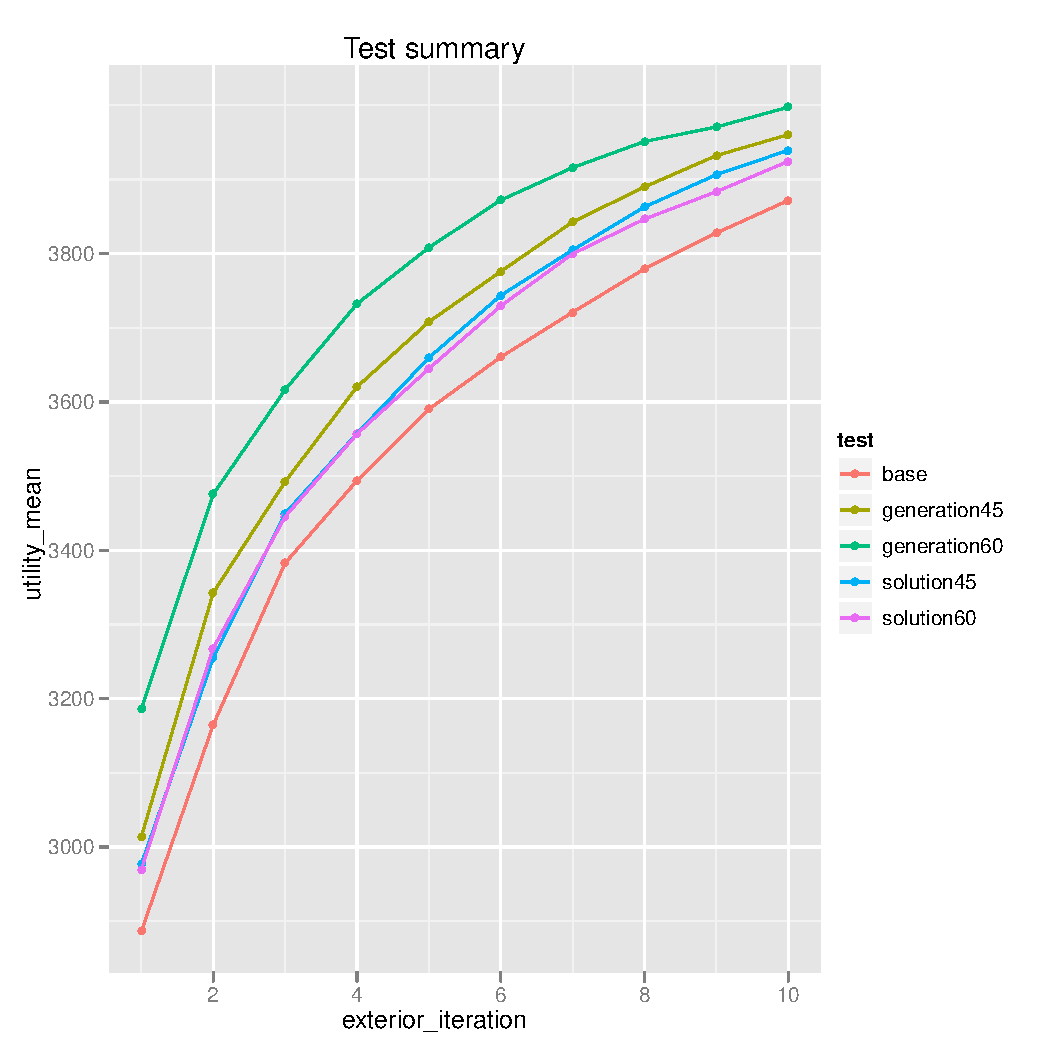
\includegraphics[width=0.65\textwidth]{exp/nouncert/c2_params1}
      \label{c2_params1}
    }
    \subfloat{
      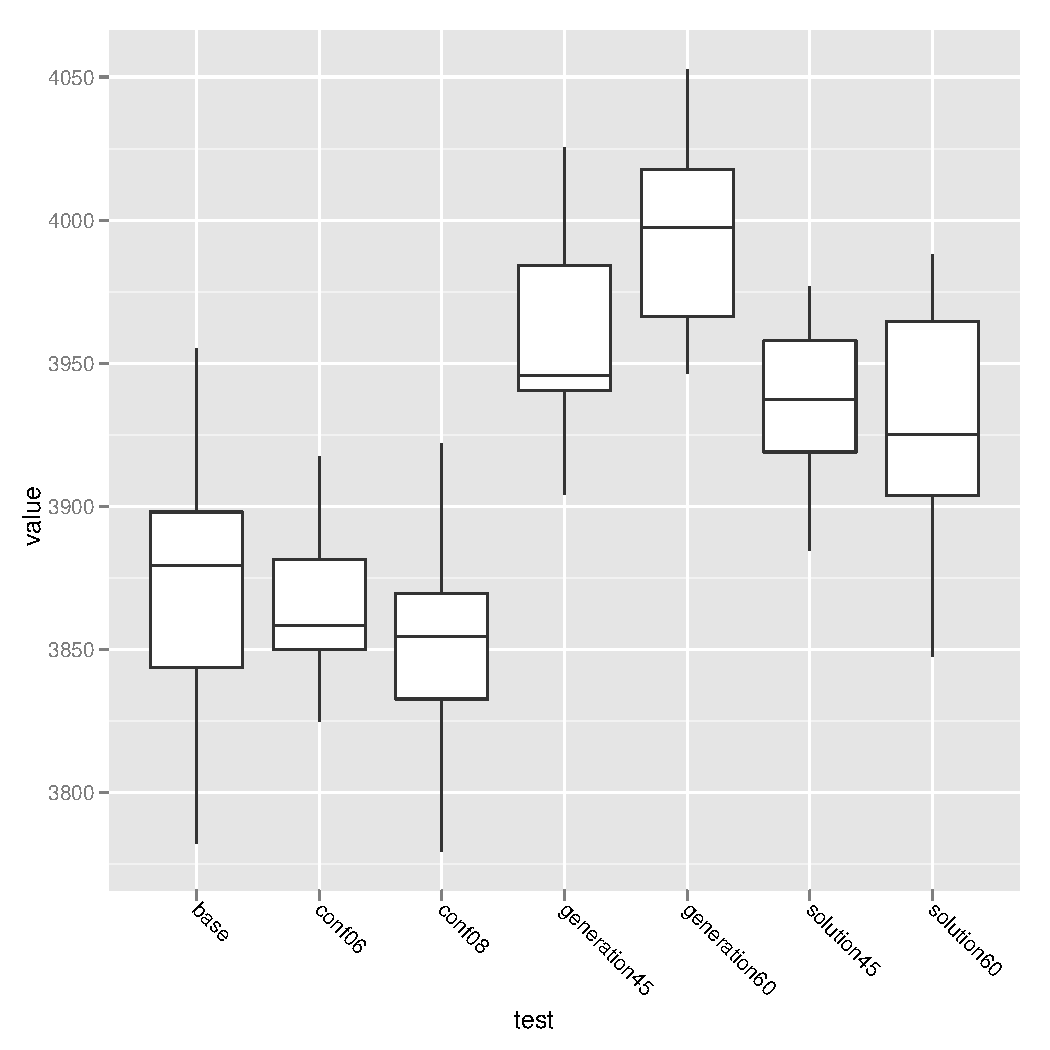
\includegraphics[width=0.65\textwidth]{exp/nouncert/c2_params1b}
      \label{c2_params1b}
    }
  }
  \caption{Basic parameters for the two-criteria binary knapsack problem}
  \label{c2_params}
\end{figure}

\begin{figure}
  \centering
  \makebox[\textwidth]{
    \subfloat{
      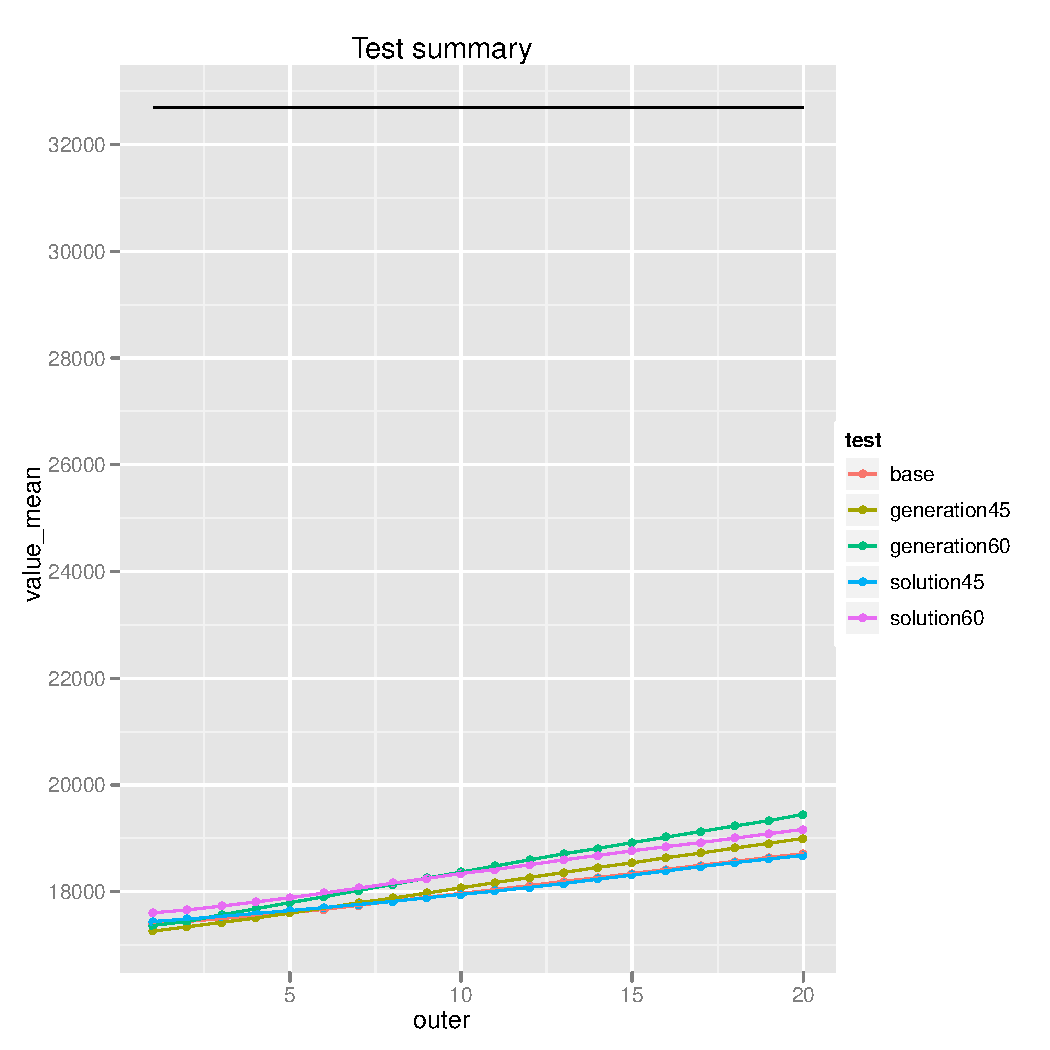
\includegraphics[width=0.65\textwidth]{exp/nouncert/c2_cont_params1}
      \label{c2_cont_params1}
    }
    \subfloat{
      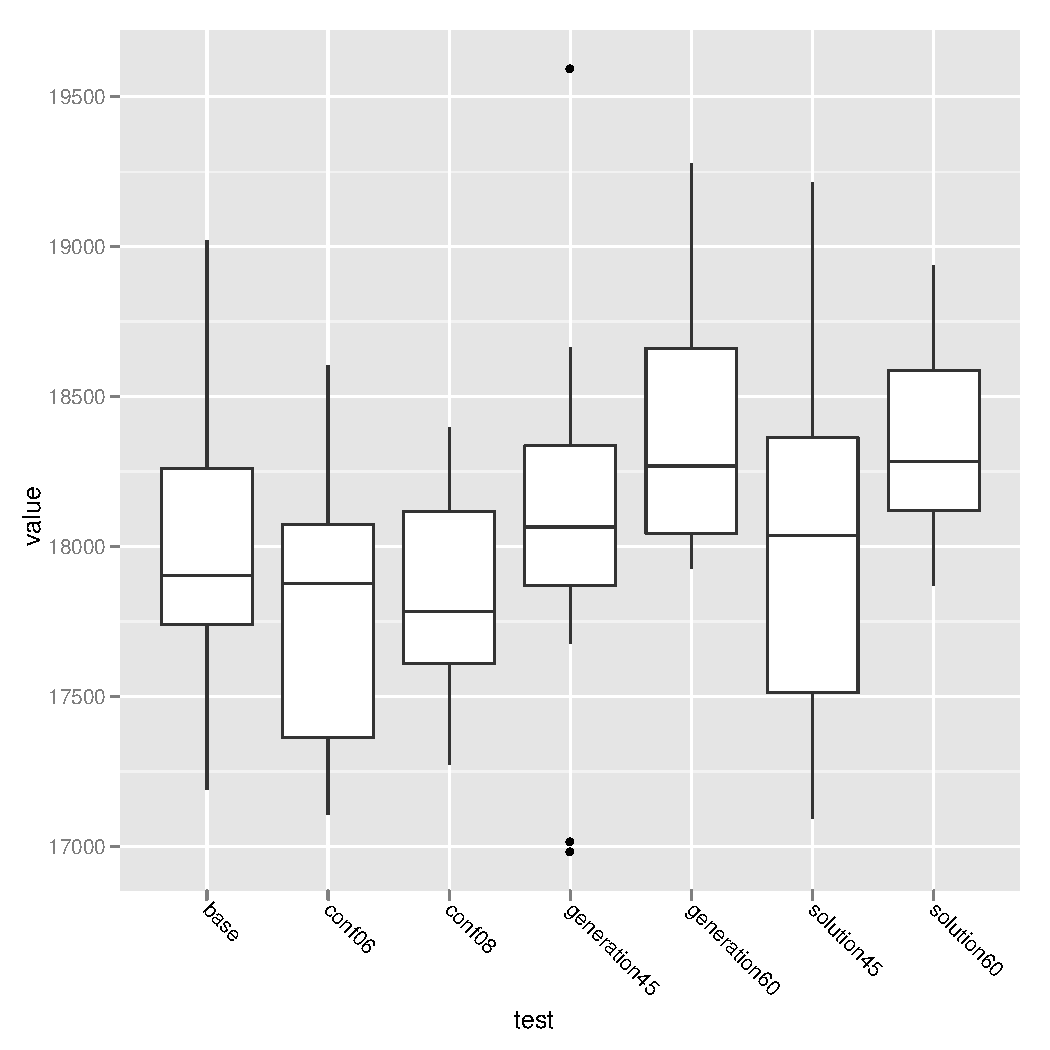
\includegraphics[width=0.6\textwidth]{exp/nouncert/c2_cont_params1b}
      \label{c2_cont_params1b}
    }
  }
  \caption{Basic parameters for the two-criteria continuous knapsack problem}
  \label{c2_cont_params}
\end{figure}

\begin{figure}
  \centering
  \makebox[\textwidth]{
    \subfloat{
      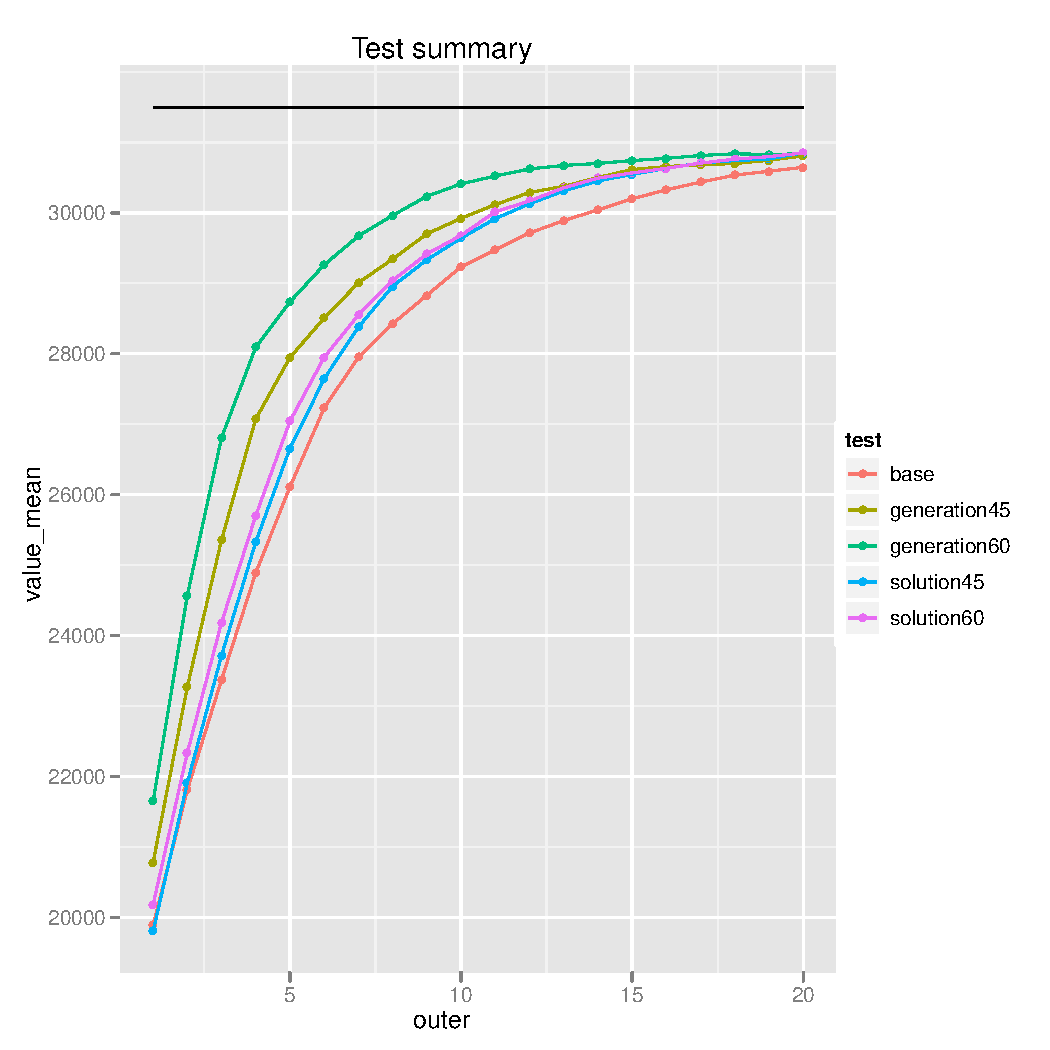
\includegraphics[width=0.65\textwidth]{exp/nouncert/c3_params1}
      \label{c3_params1}
    }
    \subfloat{
      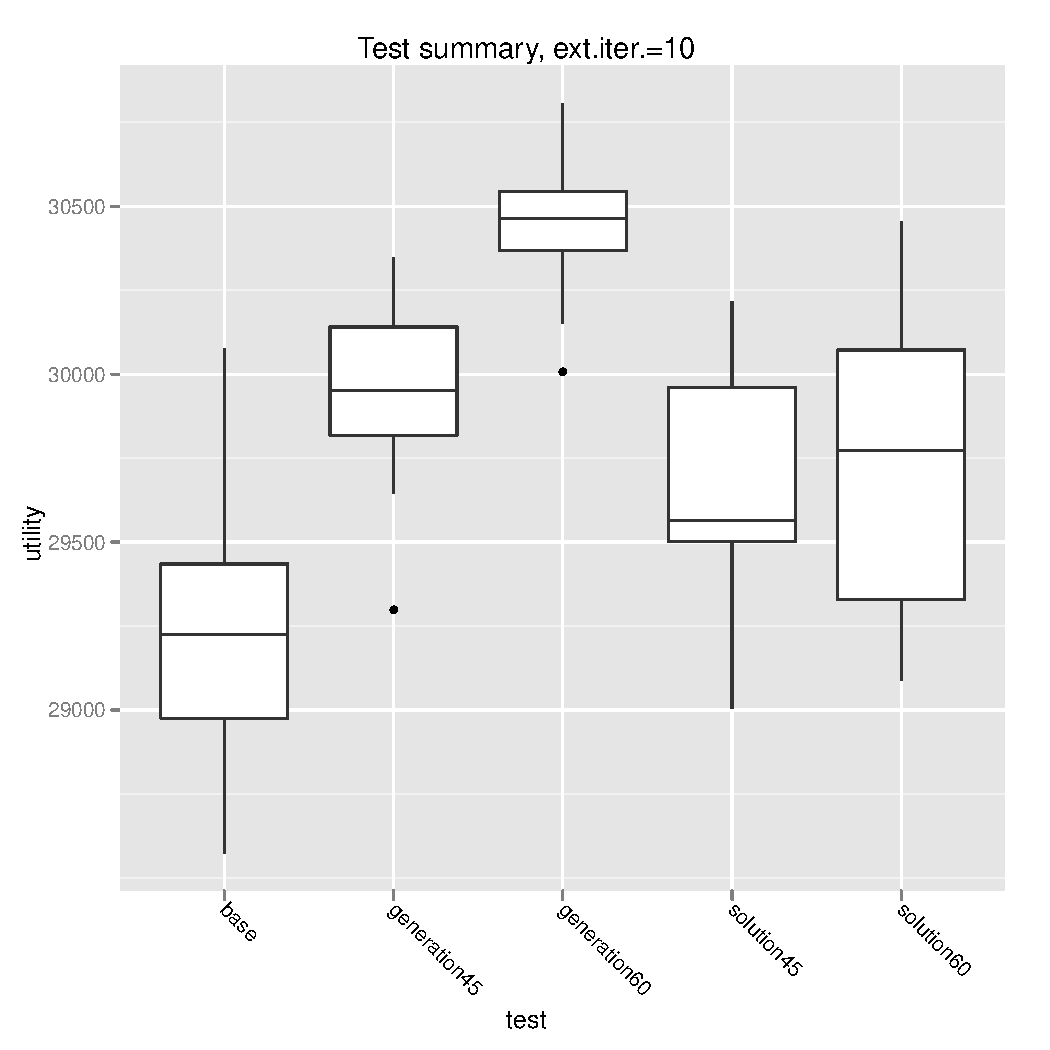
\includegraphics[width=0.6\textwidth]{exp/nouncert/c3_params1b}
      \label{c3_params1b}
    }
  }
  \caption{Basic parameters for the three-criteria binary knapsack problem}
  \label{c3_params}
\end{figure}

\begin{figure}
  \centering
  \makebox[\textwidth]{
    \subfloat{
      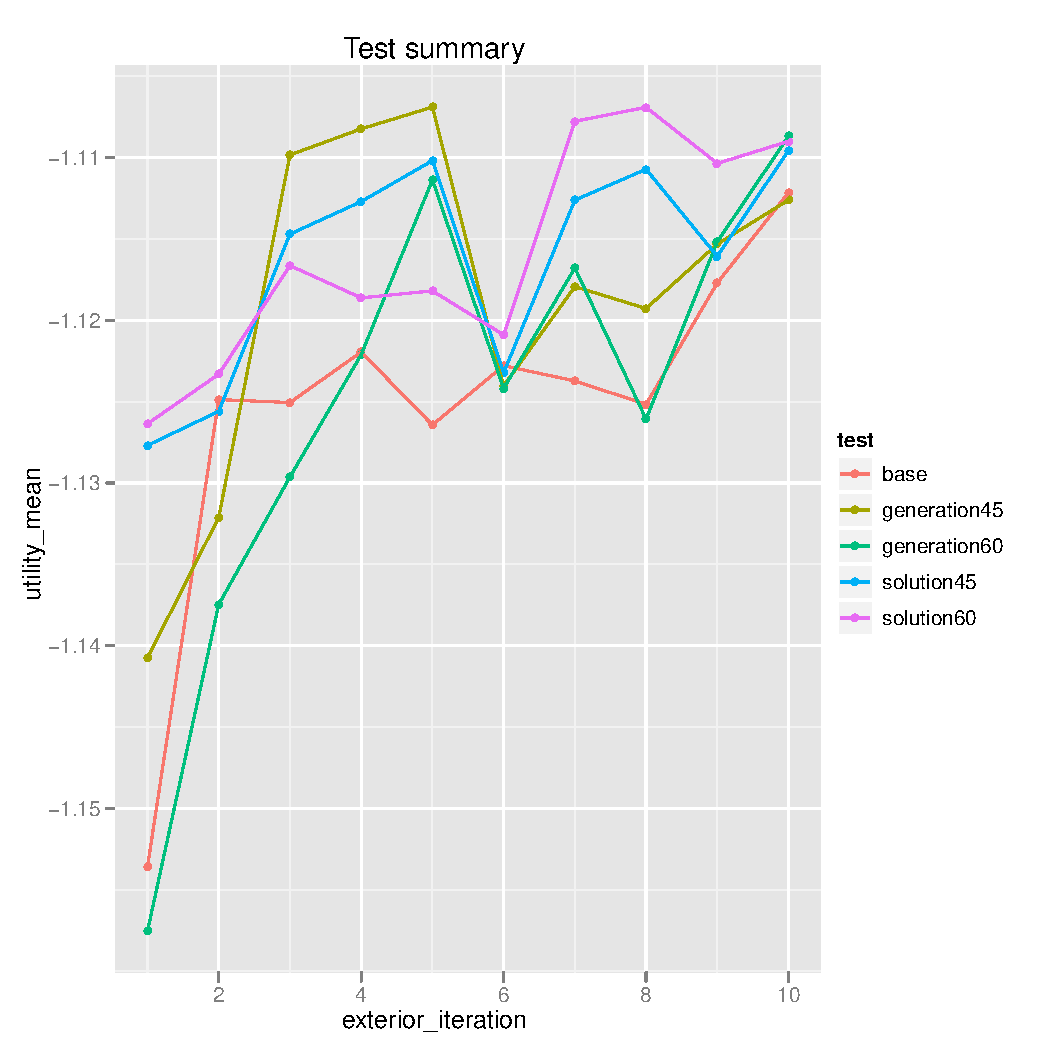
\includegraphics[width=0.65\textwidth]{exp/nouncert/c3_surface_params1}
      \label{c3_surface_params1}
    }
    \subfloat{
      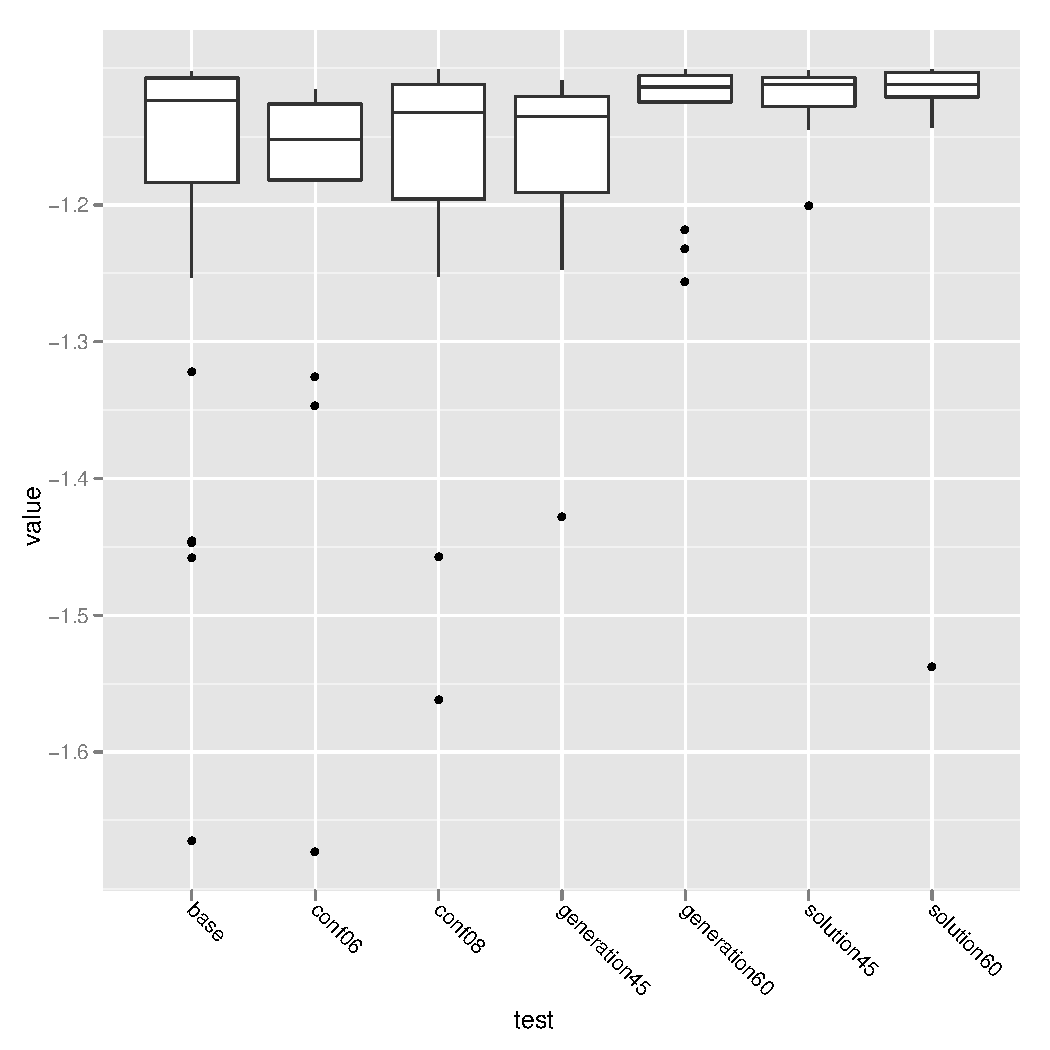
\includegraphics[width=0.6\textwidth]{exp/nouncert/c3_surface_params1b}
      \label{c3_surface_params1b}
    }
  }
  \caption{Basic parameters for the three-criteria DTLZ surface problem}
  \label{c3_surface_params}
\end{figure}


\begin{table}
  \centering
  \caption{Importance of base parameters}
  \label{t:base_imp_1}
  \begin{tabular}{r c c c c c c}
    & \multicolumn{3}{c}{Knapsack bin 2c} & \multicolumn{3}{c}{Knapsack cont 2c} \\
    \hline
    test & mean & sd & improvement & mean & sd & improvement \\
    \hline
    \hline
    base & 3870.72 & 45.73 & 0.00\% & 18711.65 & 439.25 & 0.00\% \\ 
    conf06 & 3865.89 & 26.77 & -0.12\% & 18450.09 & 559.24 & -1.40\% \\
    conf08 & 3855.53 & 40.73 & -0.39\% & 18550.45 & 389.49 & -0.86\% \\
    generation45 & 3958.75 & 34.14 & \textbf{2.27\%} & 18998.47 & 645.67 & \textbf{1.53\%} \\
    generation60 & 3995.55 & 32.71 & \textbf{3.22\%} & 19450.22 & 432.85 & \textbf{3.95\%} \\
    solution45 & 3937.89 & 26.11 & \textbf{1.74\%} & 18613.14 & 686.11 & -0.53\% \\
    solution60 & 3924.30 & 44.31 & \textbf{1.38\%} & 19169.14 & 317.48 & \textbf{2.44\%} \\
    \hline
  \end{tabular}
\end{table}

\begin{table}
  \centering
  \caption{Importance of base parameters}
  \label{t:base_imp_2}
  \begin{tabular}{r c c c c c c}
    & \multicolumn{3}{c}{Knapsack bin 3c} & \multicolumn{3}{c}{DTLZ surface 3c} \\
    \hline
    test & mean & sd & improvement & mean & sd & improvement \\
    \hline
    \hline
    base & 30648.33 & 168.22 & 0.00\% & 1.19 & 0.14 & 0.00\% \\
    conf06 & 30522.49 & 214.76 & -0.41\% & 1.21 & 0.15 & -1.24\% \\
    conf08 & 30259.30 & 201.96 & -1.27\% & 1.19 & 0.14 & -0.11\% \\
    generation45 & 30810.65 & 157.15 & \textbf{0.53\%} & 1.17 & 0.08 & \textbf{1.73\%} \\
    generation60 & 30839.93 & 110.70 & \textbf{0.63\%} & 1.14 & 0.05 & \textbf{4.61\%} \\
    solution45 & 30767.10 & 150.78 & \textbf{0.39\%} & 1.18 & 0.10 & \textbf{1.26\%} \\
    solution60 & 30852.30 & 212.38 & \textbf{0.67\%} & 1.14 & 0.11 & \textbf{4.11\%} \\
    \hline
  \end{tabular}
\end{table}


Numerical data are presented in table~\ref{t:base_imp_1}
and~\ref{t:base_imp_2}. The result are also shown on charts
(fig.~\ref{c2_params}, \ref{c2_cont_params}, \ref{c3_params}
and~\ref{c3_surface_params}). This agrees with the intuition. More solutions
(individuals in the population) and longer interior loop (more generations)
will result in better value of supposed utility for all the
problems. Confidence however yields an interesting result --- one shouldn't lower
the confidence (the default is $100\%$).

The other parameters are:
\begin{itemize}
\item Delta ($\delta$) --- decay of a rule weight.
\item Eta ($\eta$) --- initial mutation probability.
\item Gamma ($\gamma$) --- coefficient of elitism.
\item Omega ($\omega$) --- decay rate of the mutation.
\end{itemize}

They are used in the interior loop (see~[inref]).

\begin{figure}
  \centering
  \makebox[\textwidth]{
    \subfloat[Two-criteria binary knapsack]{
      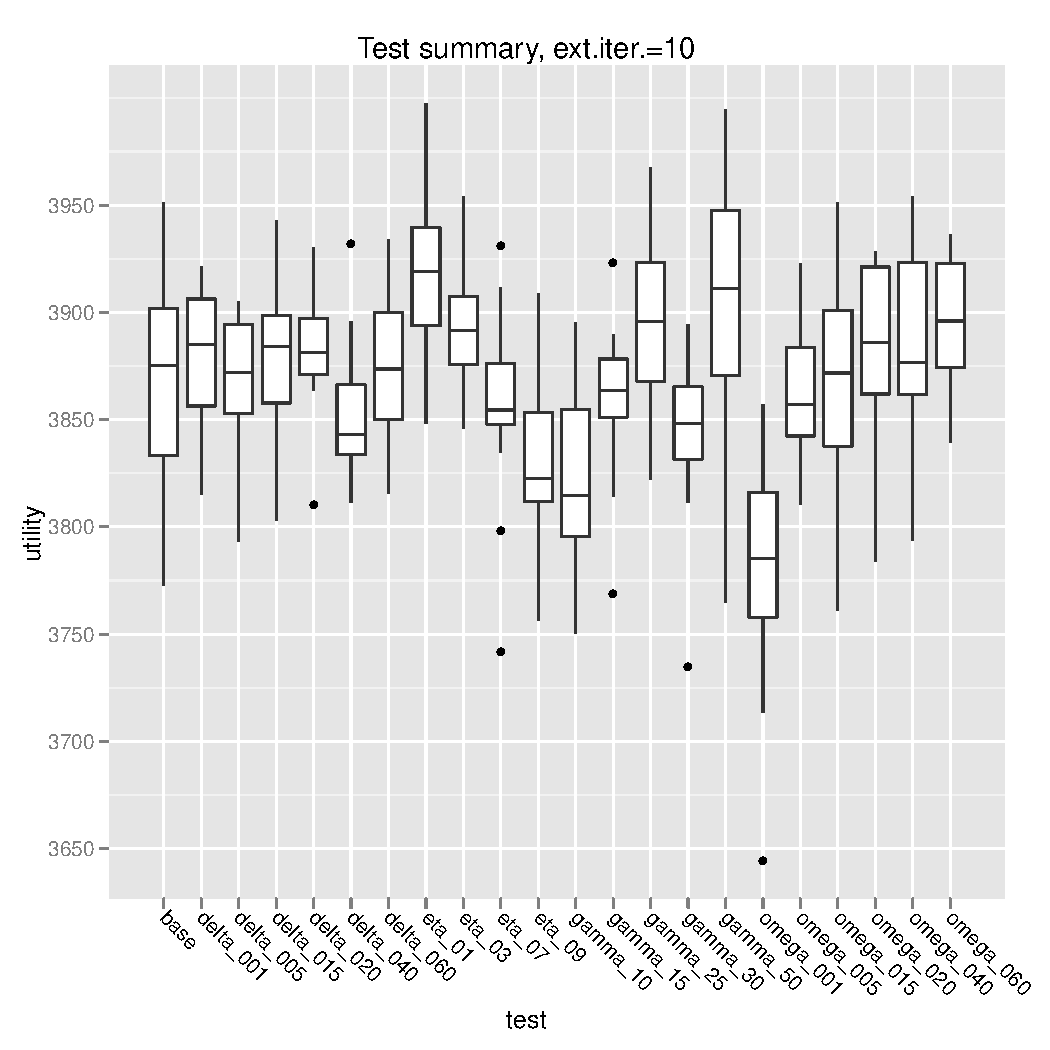
\includegraphics[width=0.60\textwidth]{exp/nouncert/c2_params2}
    }
    \subfloat[Two-criteria continuous knapsack]{
      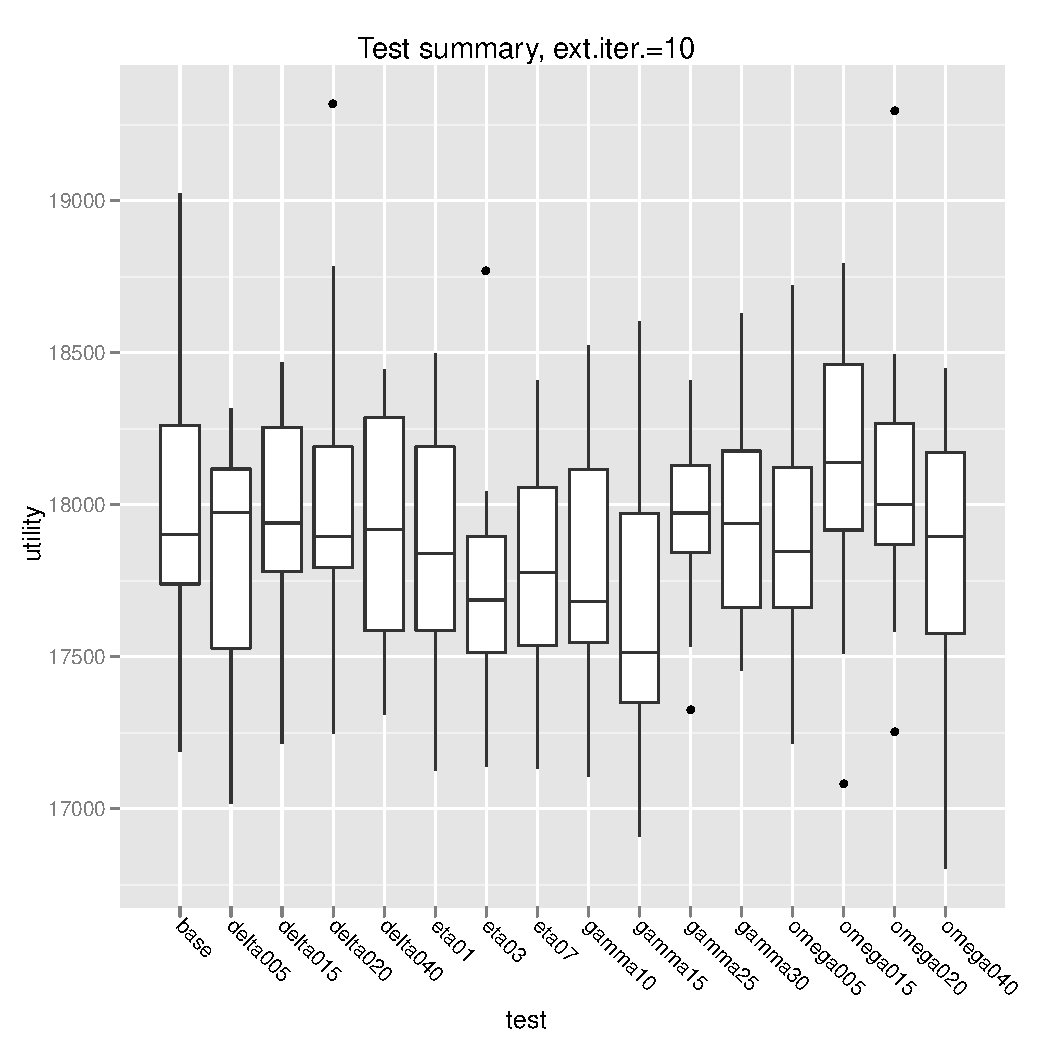
\includegraphics[width=0.60\textwidth]{exp/nouncert/c2_cont_params2}
    }
  }
  \makebox[\textwidth]{
    \subfloat[Three-criteria binary knapsack]{
      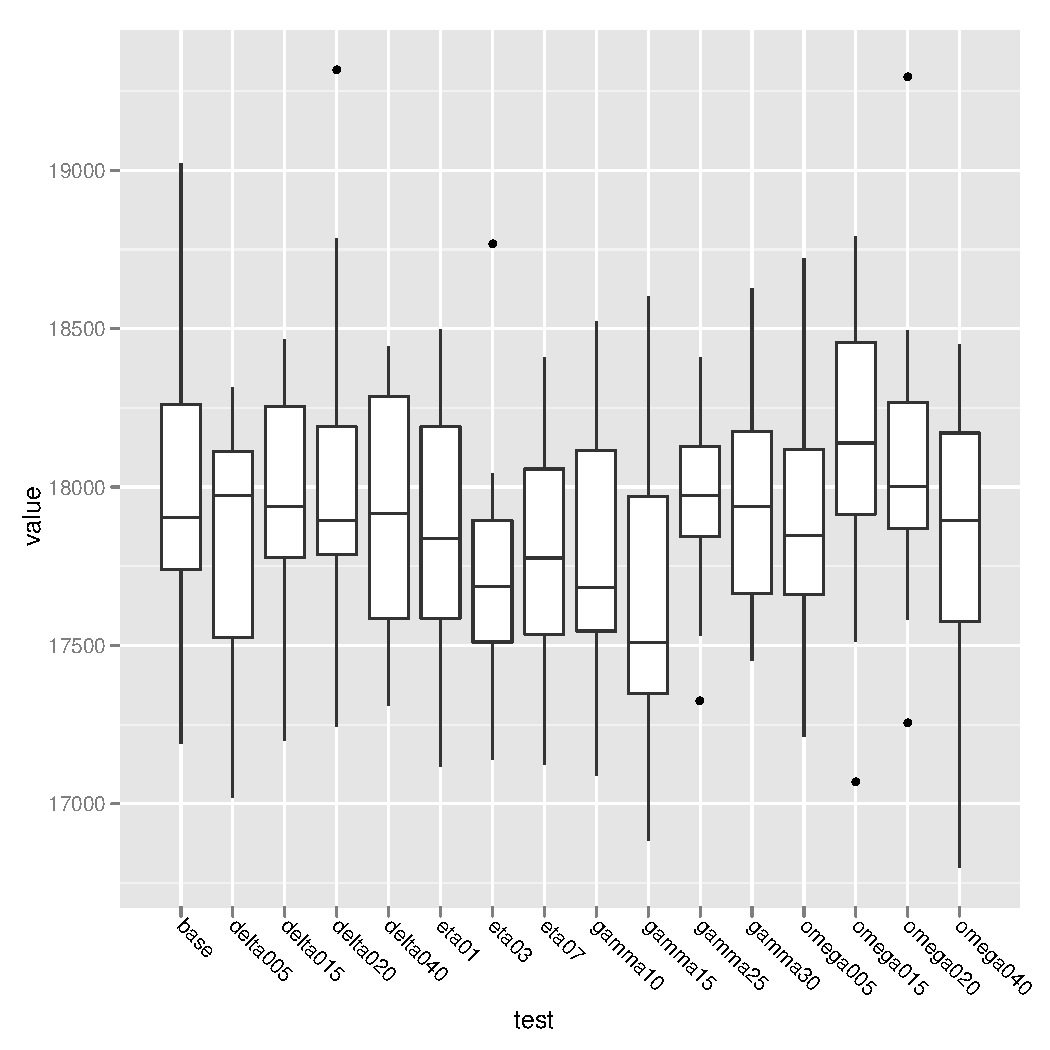
\includegraphics[width=0.60\textwidth]{exp/nouncert/c3_params2}
    }
    \subfloat[DTLZ surface problem]{
      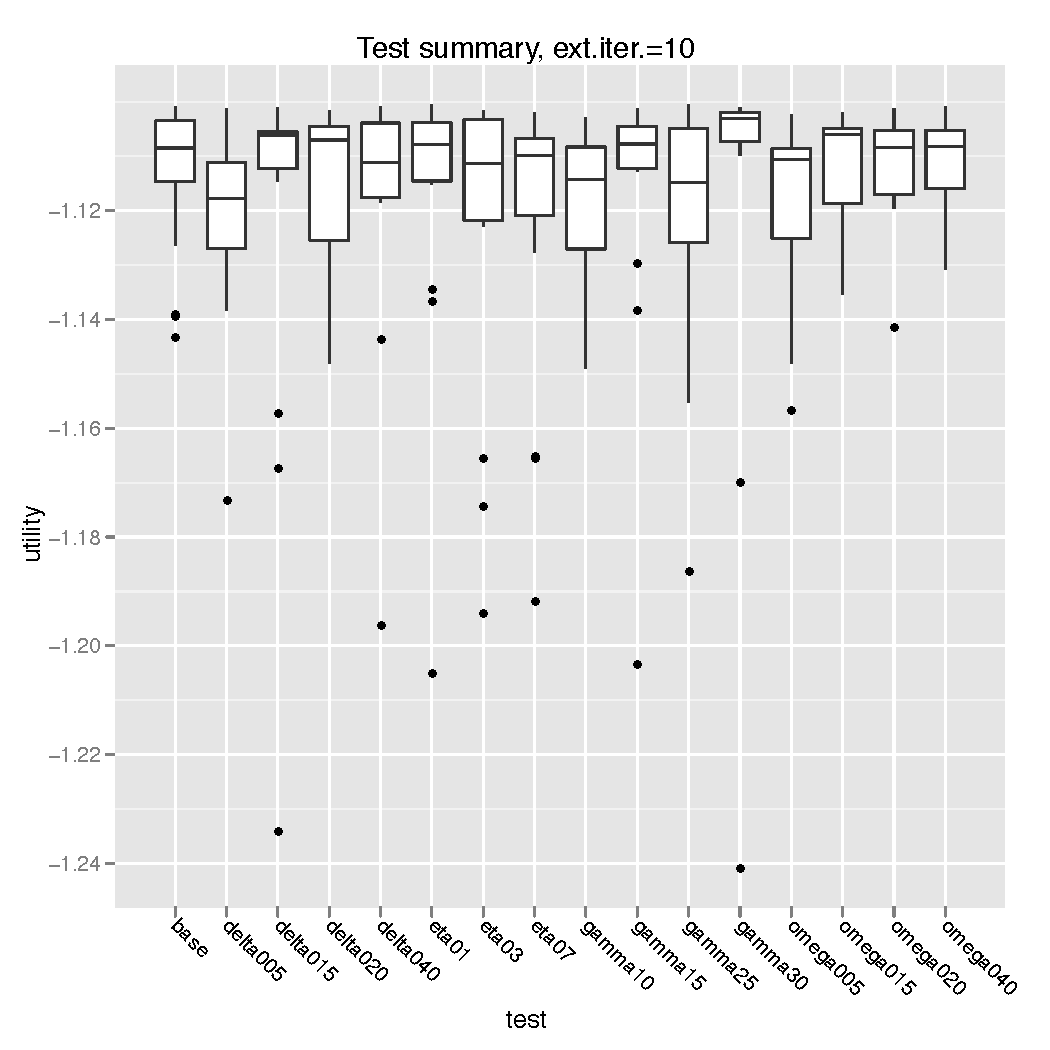
\includegraphics[width=0.60\textwidth]{exp/nouncert/c3_surface_params2}
    }
  }
  \caption{Other parameters for the three-criteria DTLZ surface problem}
  \label{params2}
\end{figure}

There is no clear patter through the problems. In general changing the other
parameters have only a minor influence over the algorithm. This is a good
think, because the solution given to the DM is robust. However analyst should
try to tune the parameters on problem basis. 

\subsection{Noise in the DM's decisions}

In the experiments performed the decision maker was mocked by a computer
algorithm. Its choices were based on assumed supposed utility function. Always
repeatable and always complying with the assumed function. This is not the
case in real-world situation where the DM is a human being and the supposed
utility function is not known. His or her decisions will be noisy, not the
best, sometimes even contradictory.

For this reason it is important to measure the impact of a ``noise'' in the
DM's choices on the algorithm. Normally, without introducing an artificial
noise the decisions are carried as follows:

\begin{algorithm}
\caption{Mocked DM indicating ``good'' solutions}\label{alg:dmselection}
  \begin{algorithmic}[1]
    \Procedure{SelectGoodSolutions}{solutions, toSelect} \\
    \Comment{solutions  --- a list of solutions generated in the interior
      loop} \\
    \Comment{toSelect --- how many solutions should be marked as ``good''}
    \ForAll{$s \in \text{solutions}$}
    \State $s.$value $\gets$ \Call{SupposedUtilityFunction}{$s$}
    \EndFor
    \State solutions $\gets$ \Call{Sort}{key=value, descending=True} \\
    \Comment{Sort solutions on descending supposed utility}
    \State \textbf{return} \Call{GetFirst}{solutions, toSelect}
    \EndProcedure
  \end{algorithmic}
\end{algorithm}

and the \textit{toSelect} parameter is set to $3$ so always three solutions
are marked as good. One can influence the behaviour of
\textsc{SelectGoodSolutions} by changing the toSelect parameter. But this is
not enough to simulate human-made noise.

First note that one do not have to always select the same number of
solutions. In fact this is unrealistic because the decision maker will select
as many solutions as he or she will think are appropriate. To mock this
behaviour additional parameter was added --- toSelectDelta. Now number of
solutions to be selected be taken from $[\text{toSelect} -
  \text{toSelectDelta}, \text{toSelect} + \text{toSelectDelta}]$ with uniform
distribution.

Second thing is that the human decision maker is fallible. He or her can make
wrong decision and not select best solutions according to supposed utility
function. Another parameter was introduced to simulate this phenomenon ---
noiseLimit. After sorting the solutions based on the supposed utility value
the individuals $1, 2, \dots, \text{noiseLimit}$ are shuffled. So lets say one
want to select three solutions. If the noiseLimit parameter is set to $0$ (the
default) three best solutions will be selected. However if an experimenter
sets the noiseLimit to $6$ three out of $6$ best solutions will be picked by
random.

The noisy version of the algorithm~\ref{alg:dmselection} is shown below.
\begin{algorithm}
\caption{Mocked DM indicating ``good'' solutions}\label{alg:noisydmselection}
  \begin{algorithmic}[1]
    \Procedure{NoisySelectGoodSolutions}{solutions, toSelect, toSelectDelta, 
      noiseLimit}
    \ForAll{$s \in \text{solutions}$}
    \State $s.$value $\gets$ \Call{SupposedUtilityFunction}{$s$}
    \EndFor
    \State solutions $\gets$ \Call{Sort}{key=value, descending=True}
    \State shuffled $\gets$ \Call{ShuffleFirst}{solutions, noiseLimit}
    \State toSelect$' \gets$ \Call{RandomFromInterval}{toSelect $-$
      toSelectDelta, toSelect $+$ toSelectDelta}
    \State \textbf{return} \Call{GetFirst}{shuffled, toSelect$'$}
    \EndProcedure
  \end{algorithmic}
\end{algorithm}

Following tests were performed:

\begin{tabular}{r c c c c c c c}
  \hline
  Parameter & no noise & noise$_1$ & noise$_2$ & noise$_3$ & noise$_4$ &
  noise$_5$ & noise$_6$ \\
  \hline
  \hline
  toSelect      & 3 & 3 & 3 & 3 & 5 &  3 &  3 \\
  toSelectDelta & 0 & 2 & 2 & 2 & 4 &  4 &  2 \\
  noiseLimit    & 0 & 0 & 2 & 4 & 6 & 10 & 16 \\
  \hline \\
\end{tabular}

Note that noise$_1$ to noise$_4$ are rather minor ones, noise$_5$ is medium
noise and finally noise$_6$ is a big one, unlikely to happen in practise ---
half of the solutions are considered as good. If the decision maker is careful
is his or her evaluations the algorithm will probably have to face a noise
between $1$ and $4$.

The results for the exemplary problems are shown on the charts below
(fig.~\ref{c2_noise}, \ref{c3_noise} and \ref{c3_surface_noise}). Noise tests
for the continuous knapsack are omitted --- the algorithm performs badly even
without additional noise.

\begin{figure}
  \centering
  \makebox[\textwidth]{
    \subfloat{
      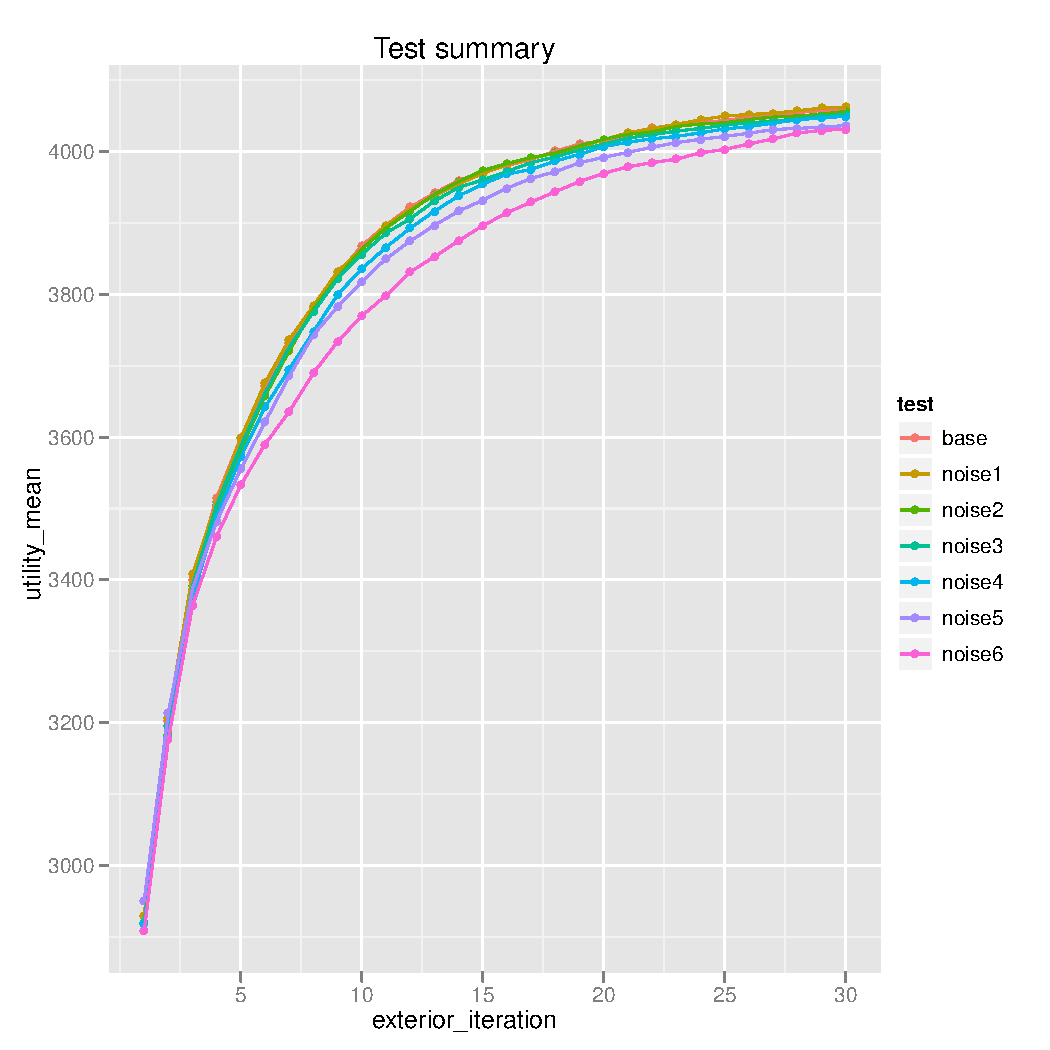
\includegraphics[width=0.65\textwidth]{exp/nouncert/c2_noise}
      \label{c2_noisea}
    }
    \subfloat{
      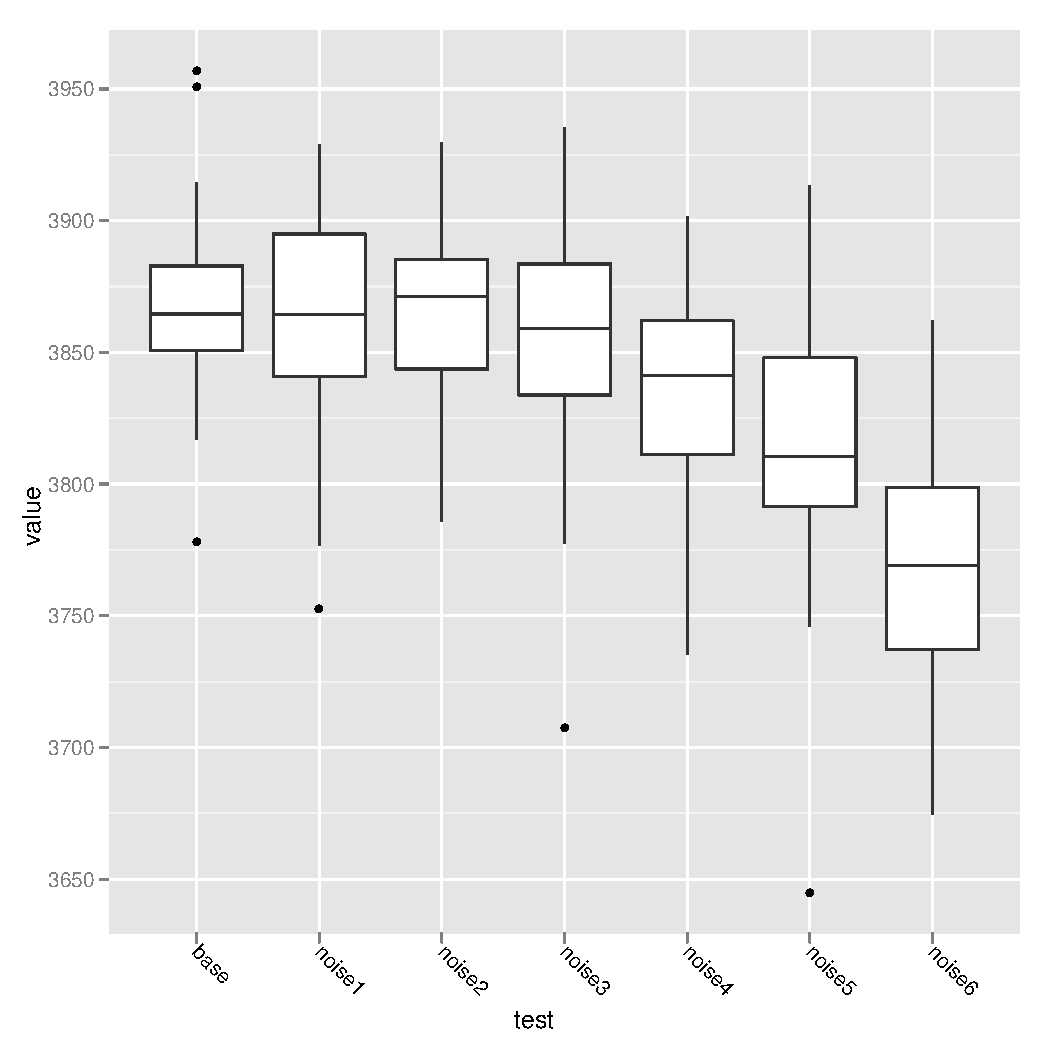
\includegraphics[width=0.65\textwidth]{exp/nouncert/c2_noiseb}
      \label{c2_noiseb}
    }
  }
  \caption{The impact of noise for the two-criteria binary knapsack problem}
  \label{c2_noise}
\end{figure}

\begin{figure}
  \centering
  \makebox[\textwidth]{
    \subfloat{
      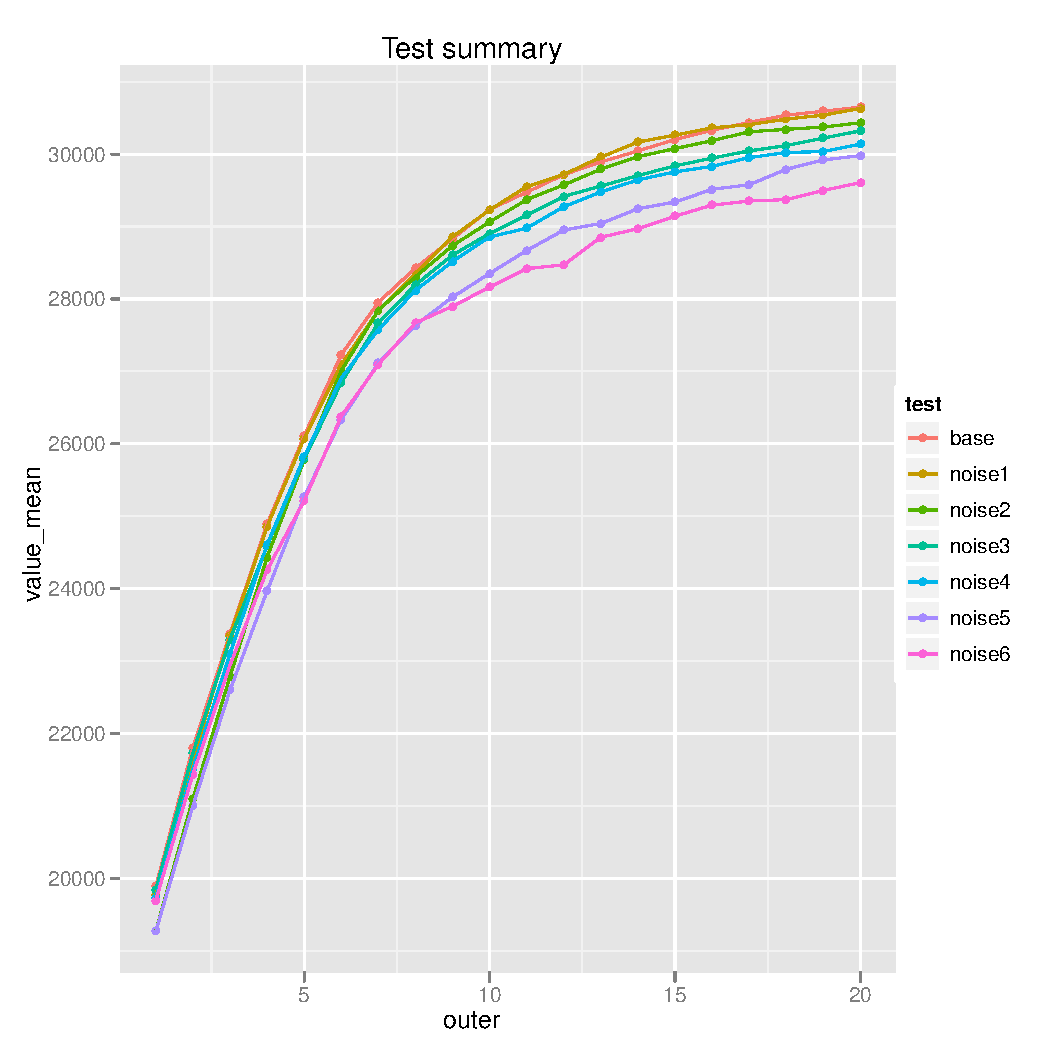
\includegraphics[width=0.65\textwidth]{exp/nouncert/c3_noise}
      \label{c3_noisea}
    }
    \subfloat{
      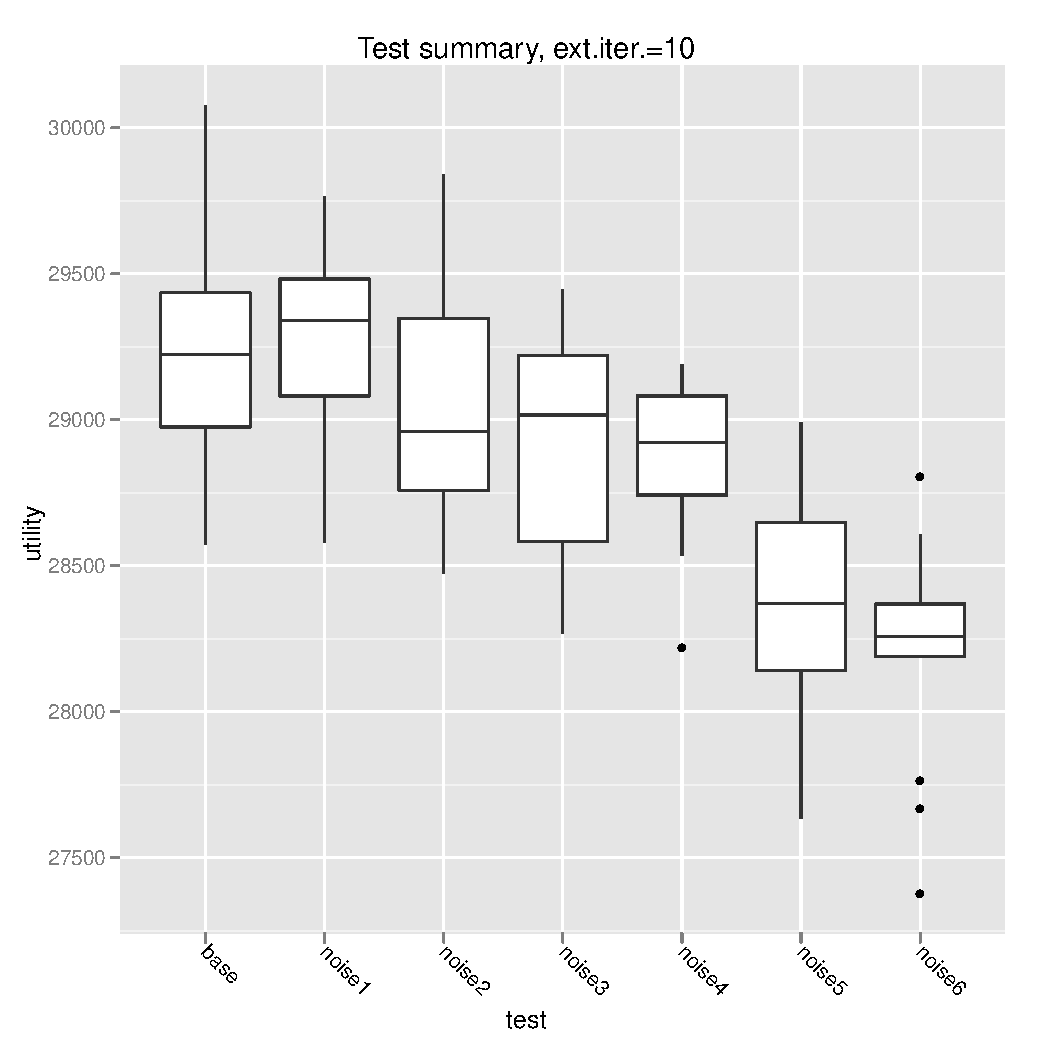
\includegraphics[width=0.65\textwidth]{exp/nouncert/c3_noiseb}
      \label{c3_noiseb}
    }
  }
  \caption{The impact of noise for the three-criteria binary knapsack problem}
  \label{c3_noise}
\end{figure}

\begin{figure}
  \centering
  \makebox[\textwidth]{
    \subfloat{
      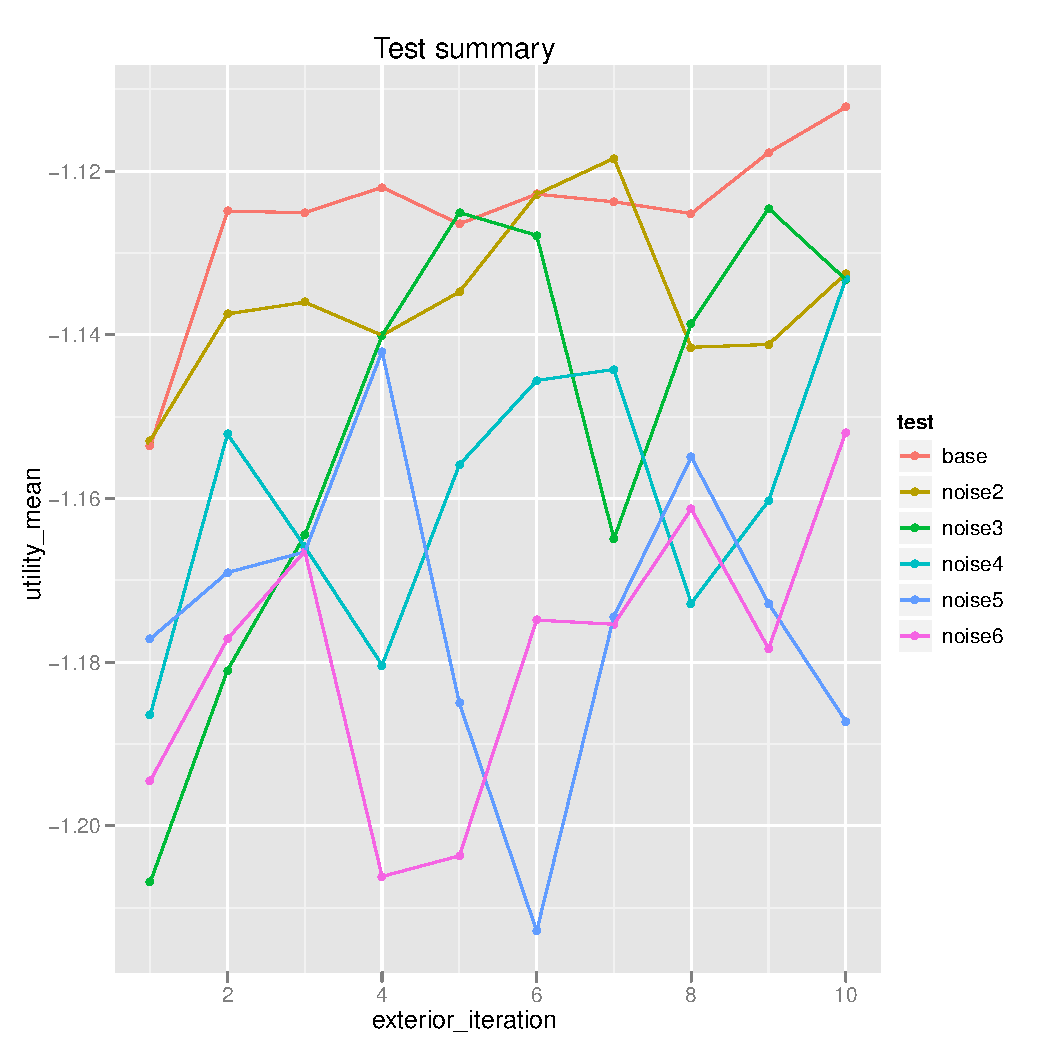
\includegraphics[width=0.65\textwidth]{exp/nouncert/c3_surface_noise}
      \label{c3_surface_noisea}
    }
    \subfloat{
      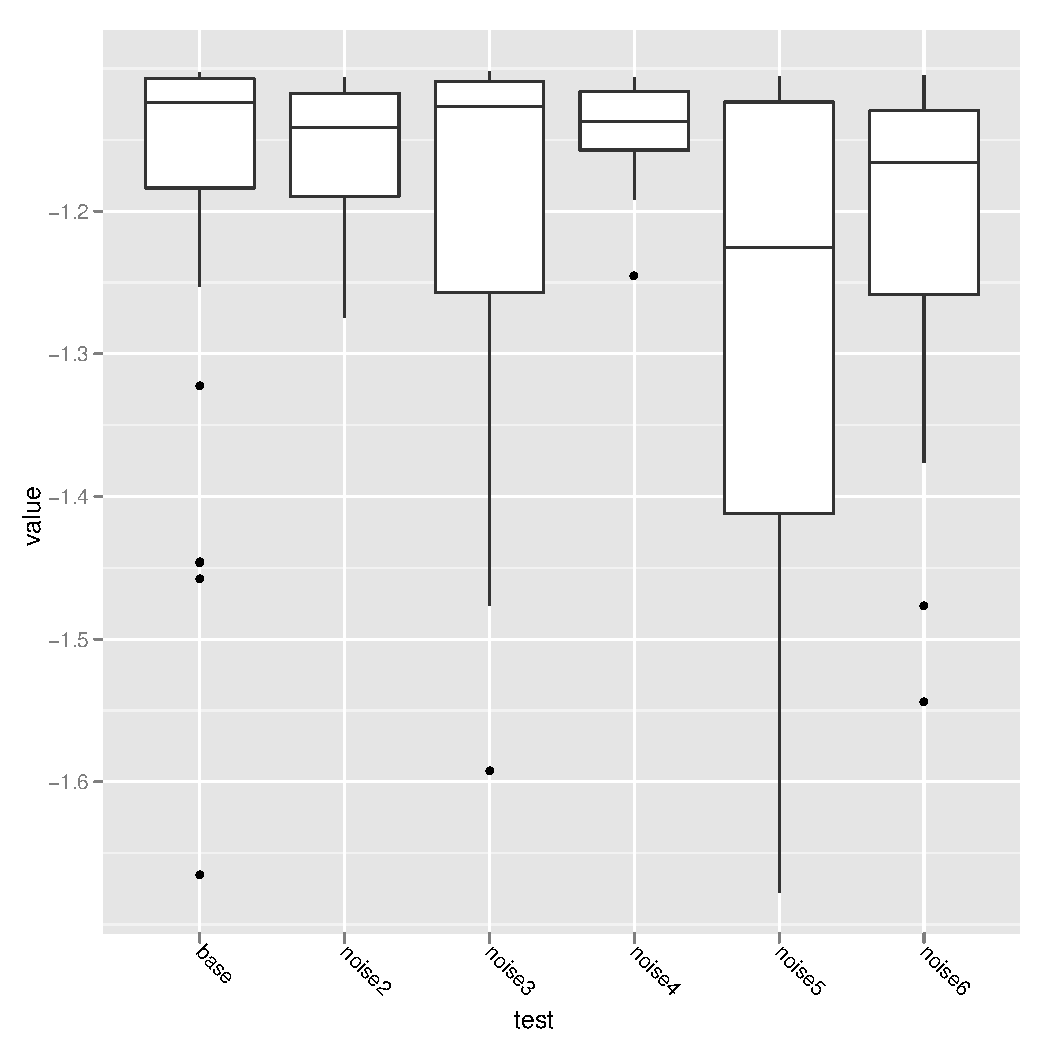
\includegraphics[width=0.65\textwidth]{exp/nouncert/c3_surface_noiseb}
      \label{c3_surface_noiseb}
    }
  }
  \caption{The impact of noise for the three-criteria DTLZ surface problem}
  \label{c3_surface_noise}
\end{figure}

Results of the DTLZ surface problem (table~\ref{t:noise} and
fig.\ref{c3_surface_noise}) are inconclusive. This is because of the behavior
described in section~\ref{nouncert-performance} --- the decision rules are not
discriminating enough so that often the utility value drops between the
interior loops. This can be seen as a form of noise with even bigger impact
than the one tested here, so it obscures results for this particular problem.

For the other problems however --- binary knapsacks (fig.~\ref{c2_noise} and
\ref{c3_noise}) the results are clear. Minor noises make almost no harm to the
results, while medium and major have only a small impact --- the value has
decreased less than $1\%$. This means that the solution generated by the
DARWIN is robust with respect to the noise in the decision maker chooses. Even
with the major noise the algorithm is able to return the same results however
a few iterations later.

\begin{table}[h]
  \centering
  \caption{The impact of noise on knapsack bin 2c}
  \label{t:noise1}
  \begin{tabular}{r c c c}
    \hline
    test & mean & sd & improvement \\
    \hline
    \hline
    base & 4057.34 & 21.31 & 0.00\% \\
    noise1 & 4061.20 & 20.45 & 0.10\% \\
    noise2 & 4055.07 & 22.89 & -0.06\% \\
    noise3 & 4049.89 & 23.98 & -0.18\% \\
    noise4 & 4044.00 & 33.41 & -0.33\% \\
    noise5 & 4032.45 & 34.63 & -0.61\% \\
    noise6 & 4029.31 & 32.76 & -0.69\% \\
    \hline
  \end{tabular}
\end{table}

\begin{table}[h]
  \centering
  \caption{The impact of noise on knapsack bin 3c}
  \label{t:noise2}
  \begin{tabular}{r c c c}
    \hline
    test & mean & sd & improvement  \\
    \hline
    \hline
    base   & 30648.33 & 168.22 & 0.00\% \\
    noise1 & 30522.49 & 214.76 & -0.41\% \\
    noise2 & 30259.30 & 201.96 & -1.27\% \\
    noise3 & 30810.65 & 157.15 & 0.53\% \\
    noise4 & 30839.93 & 110.70 & 0.63\% \\
    noise5 & 30854.91 & 86.76 & 0.67\% \\
    noise6 & 30852.30 & 212.38 & 0.67\% \\
    \hline
  \end{tabular}
\end{table}

\begin{table}[h]
  \centering
  \caption{The impact of noise on DTLZ surface 3c}
  \label{t:noise3}
  \begin{tabular}{r c c c}
    \hline
    test & mean & sd & improvement  \\
    \hline
    \hline
    base   & -1.19 & 0.14 & 0.00\% \\
    noise2 & -1.16 & 0.05 & -2.65\% \\
    noise3 & -1.21 & 0.15 & 1.46\% \\
    noise4 & -1.14 & 0.04 & -3.88\% \\
    noise5 & -1.28 & 0.17 & 7.66\% \\
    noise6 & -1.21 & 0.11 & 1.75\% \\
    \hline
  \end{tabular}
\end{table}

\clearpage{}


\section{The case of uncertainty}
In the previous sections the algorithm's results were analyzed. It was assumed
that the problems were well-specified with no room for uncertainty. It was a
way to test the algorithm's behavior and to get the idea about its properties.

It is often impossible to specify the exact values of each coefficient in the
problem. One may want to specify some of the coefficients in the form of
intervals of the possible values. Then he or she is interested in a robust
solution taking into account many possible scenarios of imprecision. This is
possible with the DARWIN method.

Now the tests performed earlier will be extended to ``robust'' problems ---
i.e.the ones with interval coefficients. Note that now it is impossible to
compare a result with the optimal solution, even assuming the supposed utility
function. However, a point of reference is needed in order to know what
performance can be expected from the method. The author decided to compare the
results with the supposed utility function optimization.

As a reference point for comparison result generated as follows was taken. The
whole exterior loop (see~\ref{idea-algo}) is left intact but in the interior loop the
goal function for evolutionary optimization changes. Instead of optimization
based on primary and secondary score the supposed utility function is the one
to be taken into account. This way it is possible to measure how well the DM's
preferences are inferred by the DARWIN method. And the preference gathering is
definitely the most important and unique part of this method.

Like in previous sections all tests were repeated at least fifteen times and
results were averaged unless stated otherwise.

\subsection{Single run analysis}
Before evaluating performances on exemplary problems it is a good idea to
analyze a single run on a single problem. It can indicate interesting
properties or potential problems of the algorithm.

The problem being evaluated is a two-criteria mix problem (this the problem
presented at the original DARWIN lecture given at \textit{5th International
  Workshop on Preferences and Decisions}, Trento, April 2009). Note that
although the problem has only two-criteria in its definition it has to be
considered in a space with more dimensions. This is because the supposed
utility function is defined not in the original two-criteria space
(\textit{max} profit, \textit{min} time) but rather in a quantile space. The
function is defined as follows:
\begin{equation*}
\textit{max}: \hspace{0.2cm} \text{profit}^{1\%} + 3 * \text{profit}^{25\%} +
2 * \text{profit}^{50\%} - \text{time}^{1\%} - 3 * \text{time}^{25\%} - 2 *
\text{time}^{50\%}
\end{equation*}

So the space has six dimensions: $p^{1\%} \times p^{25\%} \times p^{50\%}
\times t^{1\%} \times t^{25\%} \times t^{50\%}$; $t$ is for time and $p$ for
profit.

\begin{figure}
  \centering
  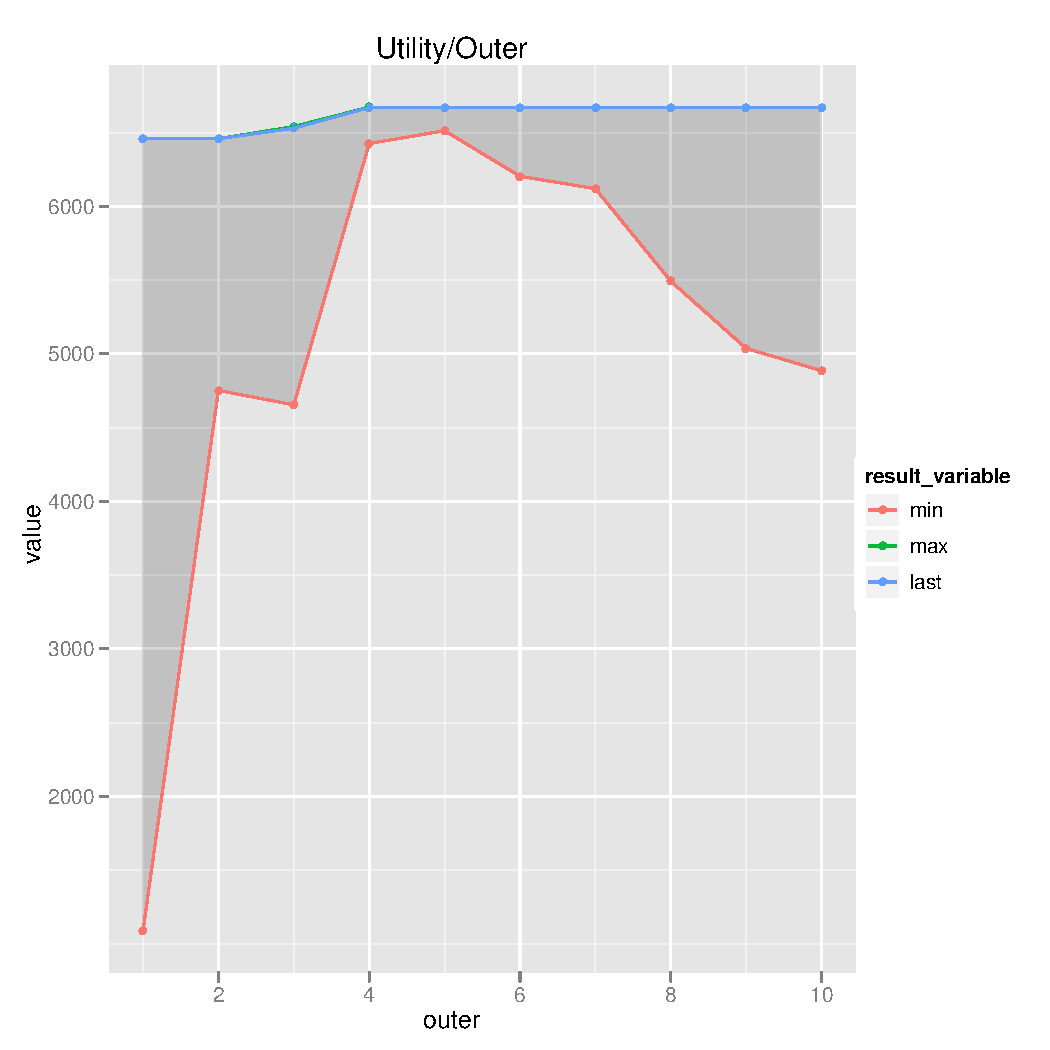
\includegraphics[width=0.8\textwidth]{exp/uncert/pres_utilouter}
  \caption{Supposed utility function in exterior loop iterations for the
    mix-problem}
  \label{pres_utilouter}
\end{figure}

Basic performance of a single run is presented in
figure~\ref{pres_utilouter}. As one can see the algorithm needs only four
iterations to reach the maximum value --- a point where no further improvement
occurs\footnote{This is not an optimal solution to the problem. By their
  nature --- intervals and scenarios of uncertainty --- a problem from this
  section does not have an optimal value.}.

Improvements of the supposed utility function and primary score are shown in
figures~\ref{pres_utilgen_01},~\ref{pres_utilgen_03} whereas the shape of the
population in fig.~\ref{pres_utilind_01},~\ref{pres_utilind_03}. One can see
that it is easy to generate a good solution to the problem --- a solution with
the best result in a given run appears in the first few generations.

Having six-dimensional objective space it is impossible to provide a section
of this space on a two-dimensional chart. However, these dimensions are not
completely independent. There is a correlation between the quantiles of the
same objective. This can be observed in fig.~\ref{pres_valweight} --- showing
the movement of population during the generation on a section of objective
space, or even better in fig.~\ref{pres_dm_choices} --- solutions marked by the
decision maker as ``good''.

As expected the solutions chosen by the DM are near the pareto-front. However,
not all of them are part of the front. Knowing that there are four other goals
besides profit$^{50\%}$ and time$^{50\%}$ explains the phenomenon.

\begin{figure}
  \centering
  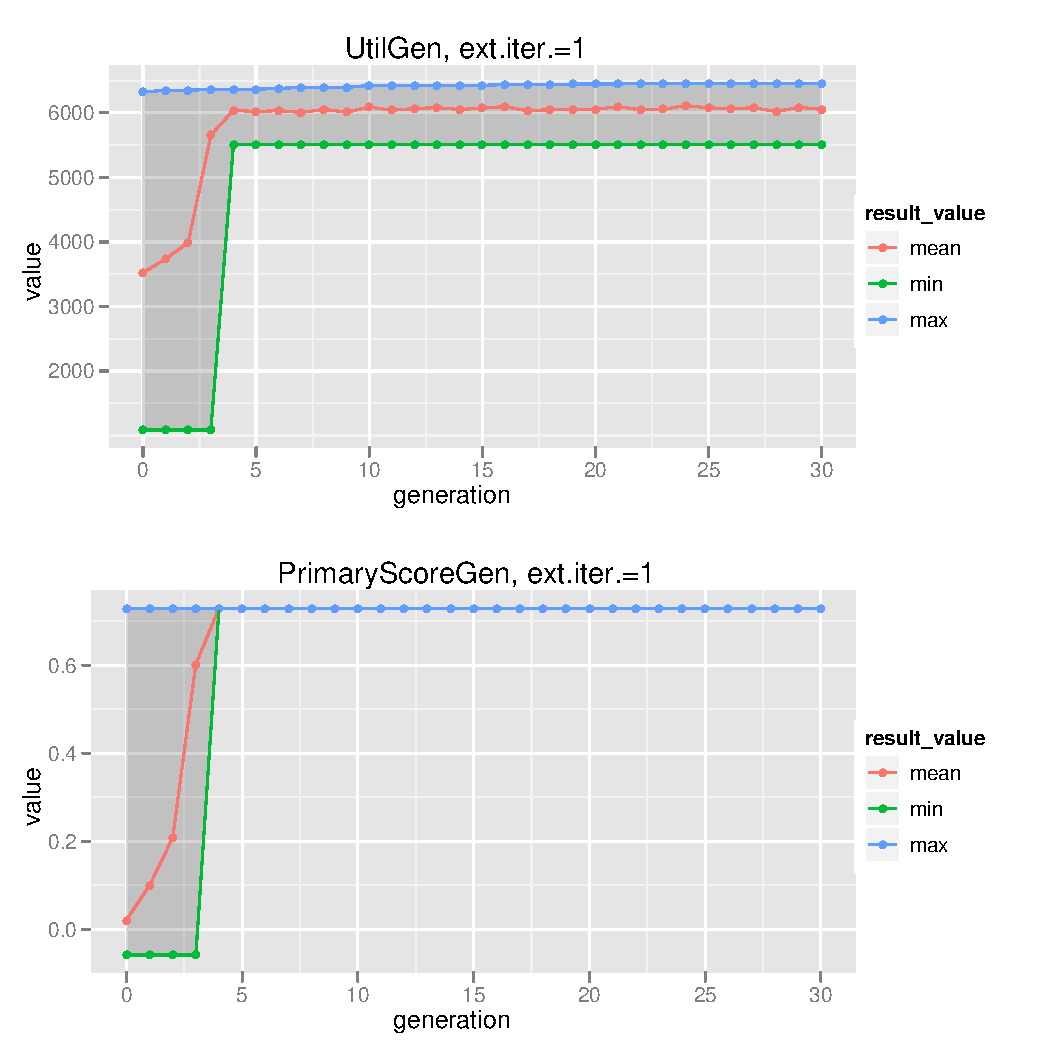
\includegraphics[width=1\textwidth]{exp/uncert/pres_utilgen_01}
  \caption{Supposed utility function and primary score improvements in an
    example run of the interior loop}
  \label{pres_utilgen_01}
\end{figure}

\begin{figure}
  \centering
  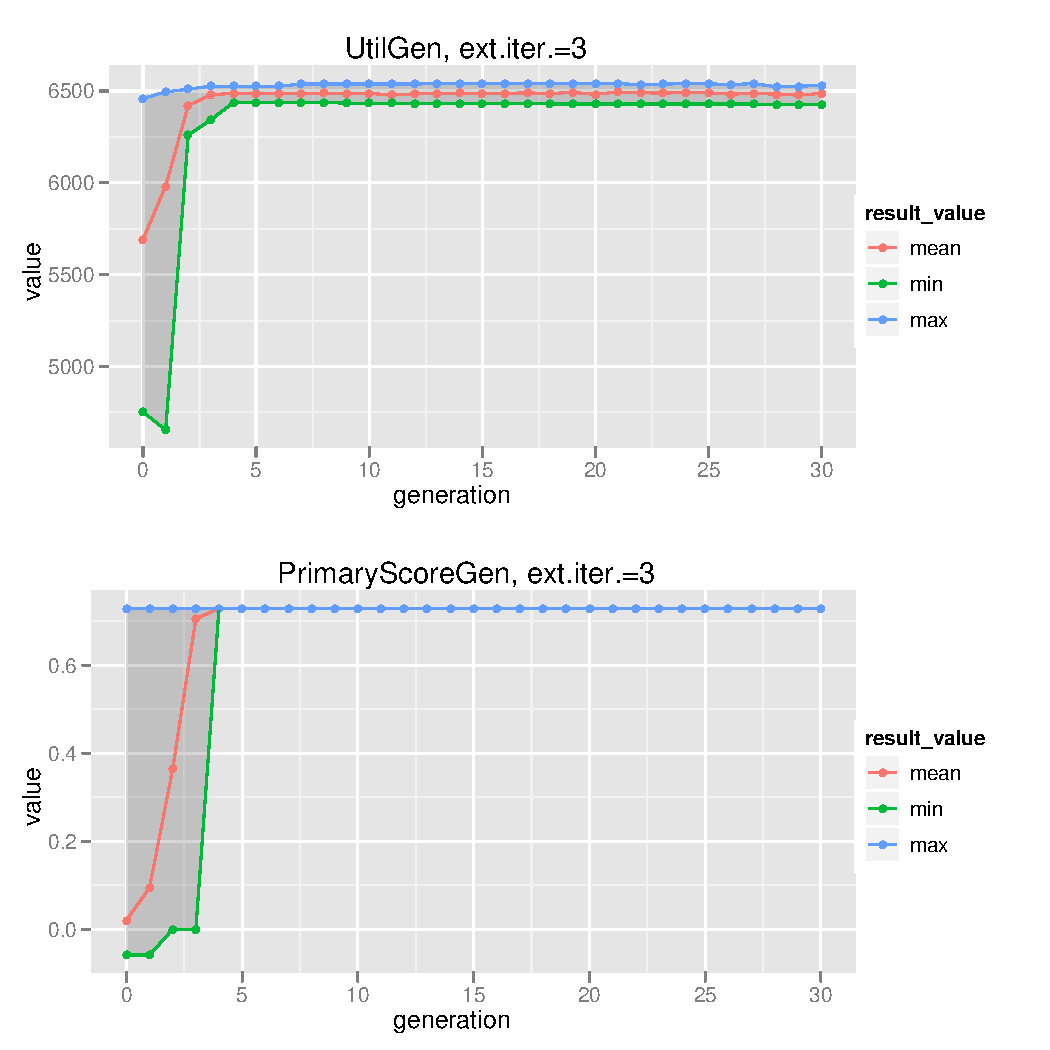
\includegraphics[width=1\textwidth]{exp/uncert/pres_utilgen_03}
  \caption{Supposed utility function and primary score improvements in an example run of the
    interior loop}
  \label{pres_utilgen_03}
\end{figure}

\begin{figure}
  \centering
  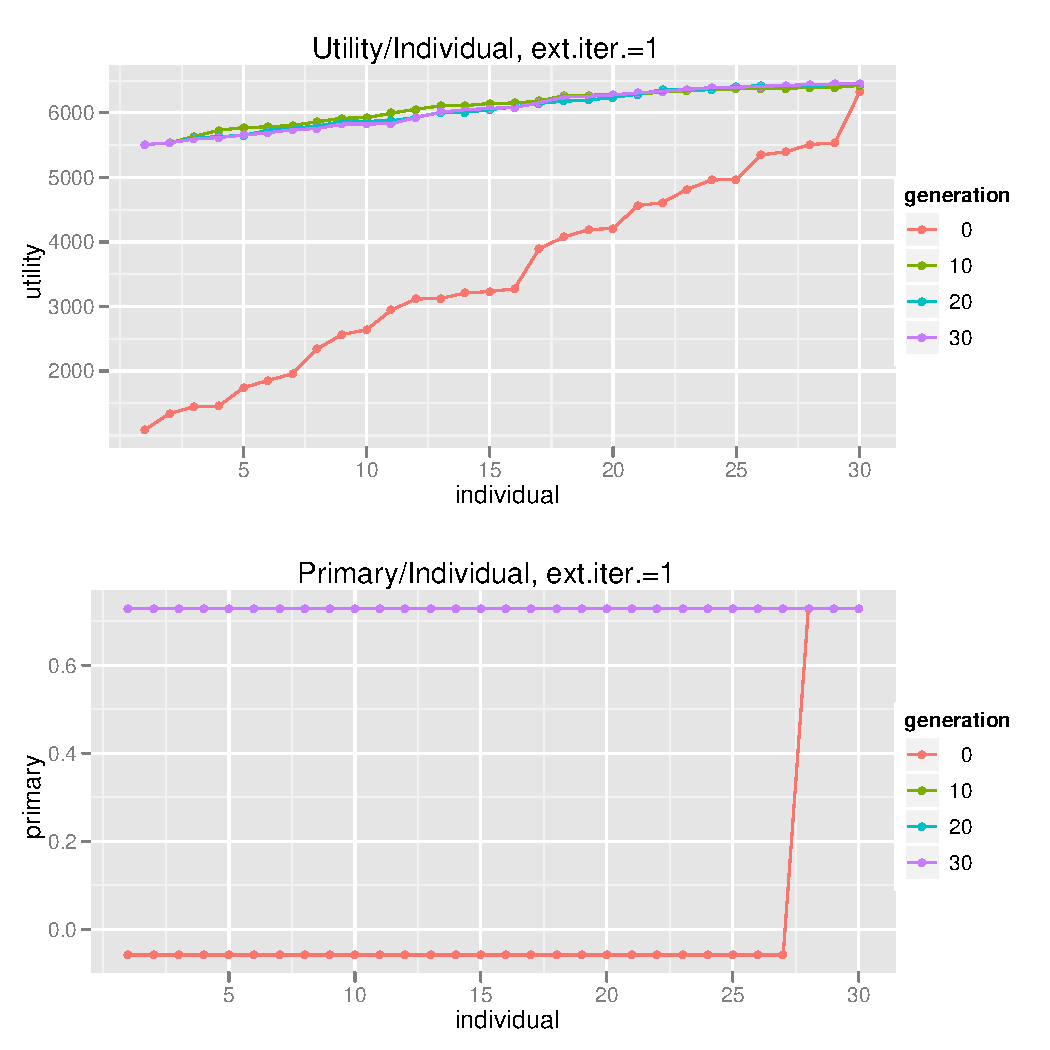
\includegraphics[width=1\textwidth]{exp/uncert/pres_utilind_01}
  \caption{Changes of the population shape in an example run of the interior
    loop}
  \label{pres_utilind_01}
\end{figure}

\begin{figure}
  \centering
  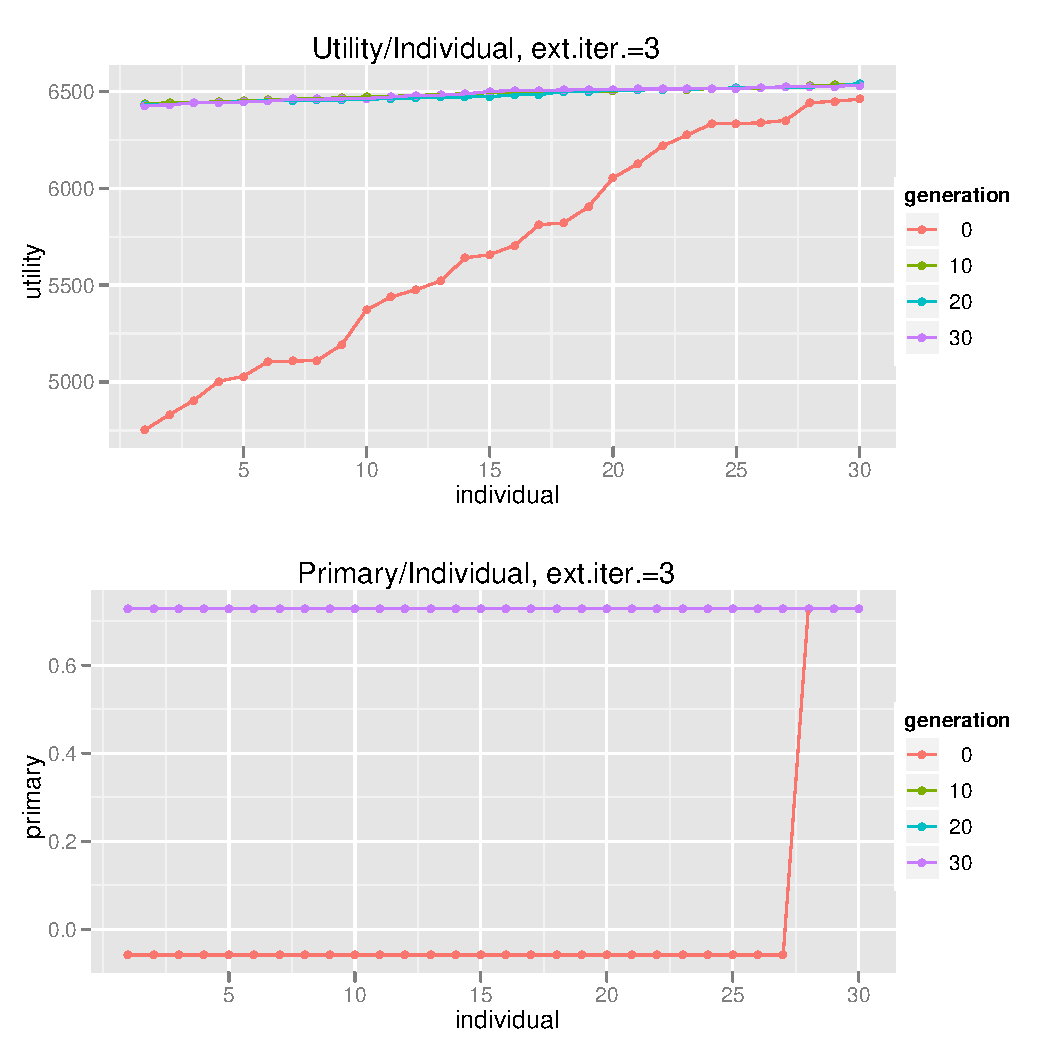
\includegraphics[width=1\textwidth]{exp/uncert/pres_utilind_03}
  \caption{Changes of the population shape in an example run of the interior
    loop}
  \label{pres_utilind_03}
\end{figure}

\begin{figure}
  \centering
  \makebox[\textwidth]{
    \subfloat{
      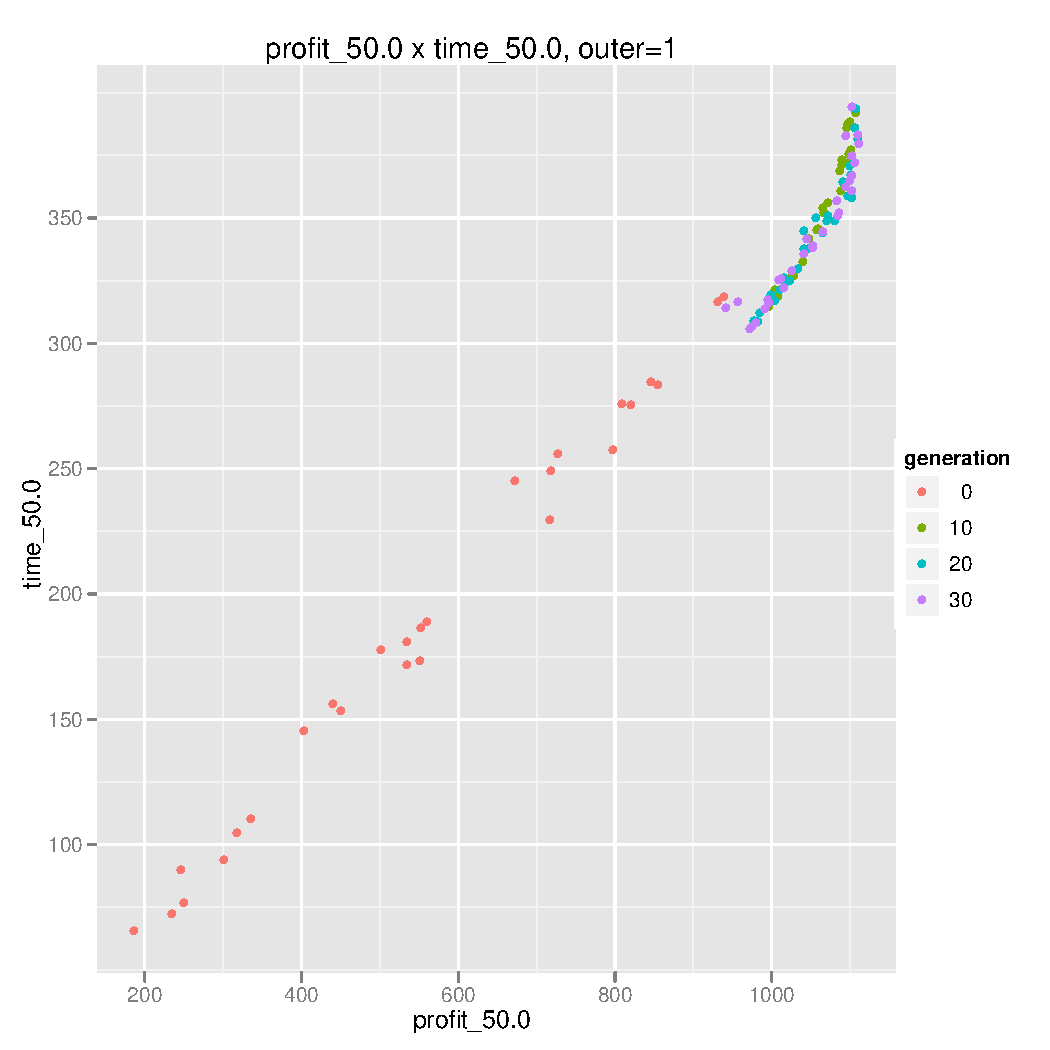
\includegraphics[scale=0.53]{exp/uncert/pres_valweight_01}
      \label{pres_valweight_01}
    }
    \subfloat{
      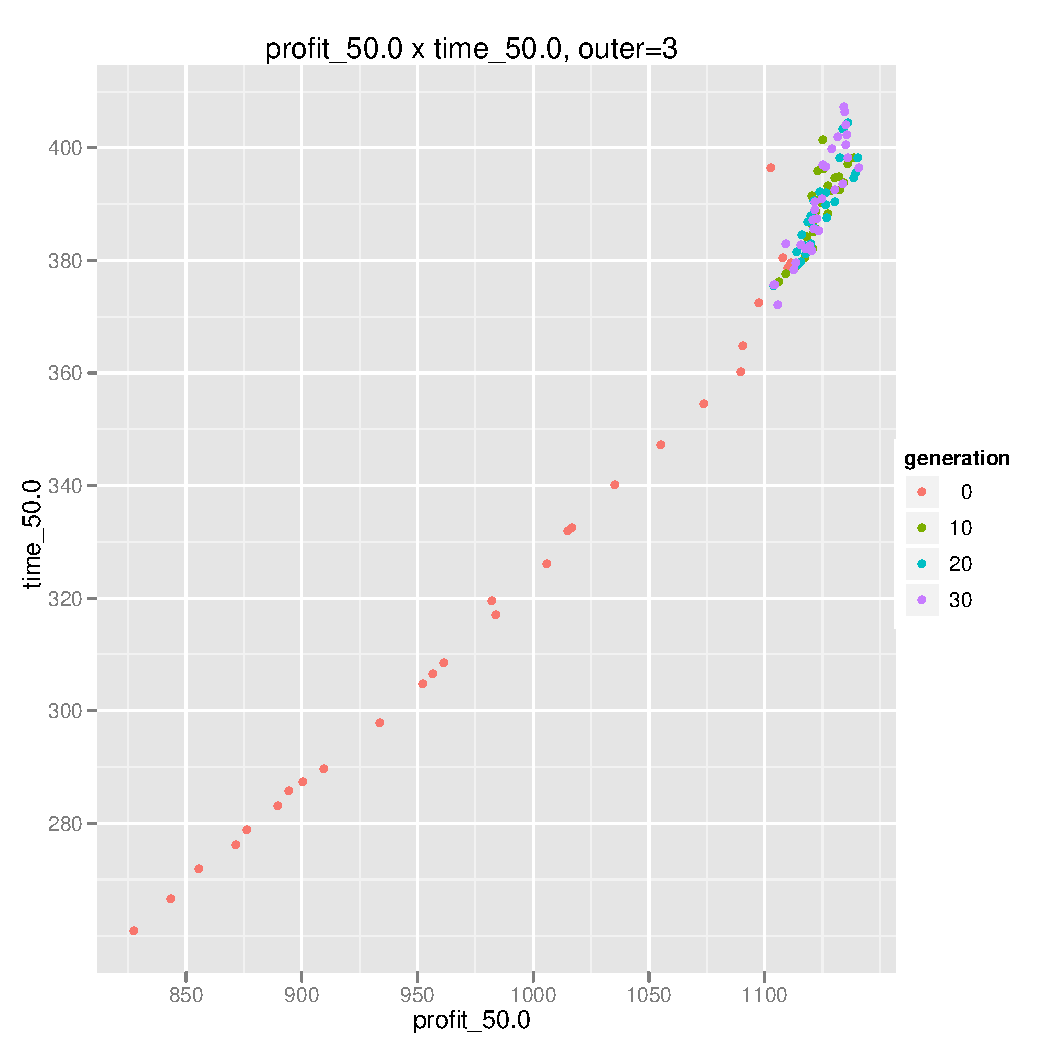
\includegraphics[scale=0.53]{exp/uncert/pres_valweight_03}
      \label{pres_valweight_03}
    }
  }
  \caption{Two-dimensional section of the objective space}
  \label{pres_valweight}
\end{figure}

\begin{figure}
  \centering
  \makebox[\textwidth]{
    \subfloat{
      \includegraphics[scale=0.53]{exp/uncert/pres_dm_choices_01}
      \label{pres_dm_choices_01}
    }
    \subfloat{
      \includegraphics[scale=0.53]{exp/uncert/pres_dm_choices_03}
      \label{pres_dm_choices_03}
    }
  }
  \caption{Two-dimensional section of the objective space}
  \label{pres_dm_choices}
\end{figure}
\clearpage{}

\subsection{The performance on exemplary problems}
To see how well DARWIN can infer the decision maker's preferences a comparison
with the supposed utility function is given. For this section the experiments
were performed on all exemplary problems with interval coefficients --- mix
problem (also labeled as presentation problem), dtlz1 (version with four and
ten-criteria) and dtlz7.

The problems were solved with default (base) values of configuration options
as well as with an increased number of generations (from $30$ to $60$). Tests
whose names end with \texttt{\_rules} are using primary and secondary score;
tests with names ending with \texttt{\_supp} are using the supposed utility
function value as an objective in evolutionary optimization.

\begin{figure}
  \centering
  \makebox[\textwidth]{
    \subfloat{
      \includegraphics[scale=0.53]{exp/uncert/pres_perf1}
      \label{pres_perf1}
    }
    \subfloat{
      \includegraphics[scale=0.53]{exp/uncert/pres_perf1b}
      \label{pres_perf1b}
    }
  }
  \caption{Performance comparison on the mix problem}
  \label{pres_perf}
\end{figure}

\begin{figure}
  \centering
  \makebox[\textwidth]{
    \subfloat{
      \includegraphics[scale=0.53]{exp/uncert/dtlz1_c4_perf1}
      \label{dtlz1_c4_perf1}
    }
    \subfloat{
      \includegraphics[scale=0.53]{exp/uncert/dtlz1_c4_perf1b}
      \label{dtlz1_c4_perf1b}
    }
  }
  \caption{Performance comparison on the four-criteria DTLZ1 problem}
  \label{dtlz1_c4_perf}
\end{figure}

\begin{figure}
  \centering
  \makebox[\textwidth]{
    \subfloat{
      \includegraphics[scale=0.53]{exp/uncert/dtlz1_c10_perf1}
      \label{dtlz1_c10_perf1}
    }
    \subfloat{
      \includegraphics[scale=0.53]{exp/uncert/dtlz1_c10_perf1b}
      \label{dtlz1_c10_perf1b}
    }
  }
  \caption{Performance comparison on the ten-criteria DTLZ1 problem}
  \label{dtlz1_c10_perf}
\end{figure}

\begin{figure}
  \centering
  \makebox[\textwidth]{
    \subfloat{
      \includegraphics[scale=0.53]{exp/uncert/dtlz7_c4_perf1}
      \label{dtlz7_c4_perf1}
    }
    \subfloat{
      \includegraphics[scale=0.53]{exp/uncert/dtlz7_c4_perf1b}
      \label{dtlz7_c4_perf1b}
    }
  }
  \caption{Performance comparison on the four-criteria DTLZ7 problem}
  \label{dtlz7_c4_perf}
\end{figure}

\begin{table}
  \centering
  \begin{tabular}{r c c c}
    \hline
    test \ optimization & supposed & rules & distance \\
    \hline
    \hline
    mix\_base & 6683.14 & 6678.95 & 0.06\% \\
    mix\_gen60 & 6680.05 & 6661.41 & 0.28\% \\
    dtlz1\_c4\_base & 7.01 & 12.81 & 45.29\% \\
    dtlz1\_c4\_gen60 & 6.48 & 15.18 & 57.28\% \\
    dtlz1\_c10\_base & 7.60 & 13.73 & 44.68\% \\
    dtlz1\_c10\_gen60 & 5.61 & 18.00 & 68.85\% \\
    dtlz7\_c4\_base & 104.72 & 108.74 & 3.69\% \\
    dtlz7\_c4\_gen60 & 104.95 & 110.28 & 4.83\% \\
    \hline
  \end{tabular}
  \caption{Performance comparison on robust multi-objective problems}
  \label{t:perf-comp}
\end{table}

The results are shown in table~\ref{t:perf-comp} and presented in
figure~\ref{pres_perf}, \ref{dtlz1_c4_perf}, \ref{dtlz1_c10_perf}
and~\ref{dtlz7_c4_perf}. There was almost no difference for the mix problem
(less than $1\%$) and a minor difference for the dtlz7 problem --- less than
$5\%$. Unfortunately, differences for dtlz1 problems (both four- and ten
criteria) were important and noticeable --- about $50\%$ percent after ten
iterations. The results for dtlz1 are far below the expectations --- the
default parameters are not appropriate for the problem. A~better result here
is still possible, however it requires tuning the parameters.

\textit{Note:} When box plots are given, they are always charted for the tenth
iteration. The same applies to comparison tables.

 \clearpage{}

\subsection{The influence of the basic parameters on the method}

The importance of basic parameters was evaluated again in the robust
environment. The numerical results are presented in the
table~\ref{t:base2_imp_1} and~\ref{t:base2_imp_2}. Also charts are included to
visualize the relations (fig.~\ref{params}).

Unfortunately, no clear pattern emerges. For a mix problem the solution is
robust --- changing the basic parameters changes the value of the result no
more than a $1\%$ after ten iterations.For the DTLZ7 problem the situation is
similar --- differences are bigger now, however still less than $5\%$.

Differences are bigger and important for the DTLZ1 problems (four- and
ten-criteria). However, the standard deviations are of the same order of
magnitude as mean values of the results. So one should say the results are
inconclusive here and it is impossible to make a suggestion based solely on
these results.

\begin{table}[htb]
  \centering
  \begin{tabular}{r c c c c c c}
    & \multicolumn{3}{c}{Mix problem} & \multicolumn{3}{c}{DTLZ1 c4} \\
    \hline
    test & mean & sd & improvement & mean & sd & improvement \\
    \hline
    \hline
    base & 6665.60 & 57.27 & 0.00\% & -9.99 & 6.83 & 0.00\% \\
    generation45 & 6661.72 & 47.52 & -0.06\% & -16.04 & 12.47 & 60.63\% \\
    generation60 & 6661.14 & 45.08 & -0.07\% & -9.63 & 7.78 & -3.61\% \\
    scenario45 & 6617.60 & 47.33 & -0.72\% & -13.12 & 11.37 & 31.34\% \\
    scenario60 & 6639.54 & 33.98 & -0.39\% & -13.95 & 8.50 & 39.68\% \\
    solution45 & 6705.68 & 52.96 & 0.60\% & -10.43 & 8.33 & 4.44\% \\
    solution60 & 6685.43 & 56.78 & 0.30\% & -11.68 & 8.23 & 16.97\% \\
    \hline
  \end{tabular}
  \caption{Importance of base parameters in robust environment}
  \label{t:base2_imp_1}
\end{table}

\begin{table}[htb]
  \centering
  \begin{tabular}{r c c c c c c}
    & \multicolumn{3}{c}{DTLZ1 c10} & \multicolumn{3}{c}{DTLZ7 c4} \\
    \hline
    test & mean & sd & improvement & mean & sd & improvement \\
    \hline
    \hline
    base & -15.30 & 11.20 & 0.00\% & -109.23 & 5.87 & 0.00\% \\
    generation45 & -15.92 & 13.27 & 4.03\% & -109.23 & 6.96 & 0.00\% \\
    generation60 & -21.63 & 12.55 & 41.37\% & -108.33 & 10.87 & -0.82\% \\
    scenario45 & -17.32 & 11.15 & 13.17\% & -111.98 & 5.34 & 2.52\% \\
    scenario60 & -16.67 & 13.30 & 8.91\% & -112.54 & 3.45 & 3.03\% \\
    solution45 & -13.89 & 9.63 & -9.22\% & -107.88 & 6.39 & -1.23\% \\
    solution60 & -9.55 & 6.81 & -37.62\% & -109.98 & 6.37 & 0.69\% \\
    \hline
  \end{tabular}
  \caption{Importance of base parameters in robust environment}
  \label{t:base2_imp_2}
\end{table}

\begin{figure}
  \centering
  \makebox[\textwidth]{
    \subfloat[Mix problem]{
      \includegraphics[scale=0.53]{exp/uncert/pres_params}
      \label{pres_params}
    }
    \subfloat[DTLZ1 four-criteria]{
      \includegraphics[scale=0.53]{exp/uncert/dtlz1_c4_params}
      \label{dtlz1_c4_params}
    }
  }
  \makebox[\textwidth]{
    \subfloat[DTLZ1 ten-criteria]{
      \includegraphics[scale=0.53]{exp/uncert/dtlz1_c10_params}
      \label{dtlz1_c10_params}
    }
    \subfloat[DTLZ7 four-criteria]{
      \includegraphics[scale=0.53]{exp/uncert/dtlz7_c4_params}
      \label{dtlz7_c4_params}
    }
  }
  \caption{Effect of params in DM's decisions}
  \label{params}
\end{figure}

\clearpage{}

\subsection{DM's decisions inconsistent with supposed utility function}
\label{noise-dm2}


In order to check the impact of a noise in DM's decisions, experiments were
performed. The results are presented in figure~\ref{noise} and in the
tables~\ref{t:un_noise_1} and~\ref{t:un_noise_2}.

Again one has to analyze the results excluding the DTLZ1 problem. This is
because of the standard deviation of the series of results --- again it is the
same order of magnitude as the value itself.

In the Mix and DTLZ7 problems the effect of the noise starts to be an
important factor only in case of medium- (noise$_5$) --- the results differ
about $8\%$ and in case of a major-noise (noise$_6$) --- difference about 12\%
for the mix problem and about 8\% for the DTLZ7 problem.

The situation is similar to the impact on problems defined without
uncertainty. Even if one adds the interval coefficients to the problem, the
solution is still robust with respect to the noise.


\begin{figure}
  \centering
  \makebox[\textwidth]{
    \subfloat[Mix problem]{
      \includegraphics[scale=0.53]{exp/uncert/pres_noise}
      \label{pres_noise}
    }
    \subfloat[DTLZ1 four-criteria]{
      \includegraphics[scale=0.53]{exp/uncert/dtlz1_c4_noise}
      \label{dtlz1_c4_noise}
    }
  }
  \makebox[\textwidth]{
    \subfloat[DTLZ1 ten-criteria]{
      \includegraphics[scale=0.53]{exp/uncert/dtlz1_c10_noise}
      \label{dtlz1_c10_noise}
    }
    \subfloat[DTLZ7 four-criteria]{
      \includegraphics[scale=0.53]{exp/uncert/dtlz7_c4_noise}
      \label{dtlz7_c4_noise}
    }
  }
  \caption{Effect of noise in DM's decisions}
  \label{noise}
\end{figure}


\begin{table}[htb]
  \centering
  \begin{tabular}{r c c c c c c}
    & \multicolumn{3}{c}{Mix problem} & \multicolumn{3}{c}{DTLZ1 c4} \\
    \hline
    noise level & mean & sd & improvement & mean & sd & improvement \\
    \hline
    \hline
    base & 6678.95 & 53.86 & 0.00\% & -12.81 & 8.38 & 0.00\% \\
    noise1 & 6662.93 & 36.54 & -0.24\% & -7.70 & 8.48 & 39.89\% \\
    noise2 & 6638.77 & 70.33 & -0.60\% & -12.61 & 11.36 & 1.55\% \\
    noise3 & 6636.90 & 53.88 & -0.63\% & -12.73 & 10.82 & 0.61\% \\
    noise4 & 6537.39 & 137.71 & -2.12\% & -13.65 & 7.84 & -6.55\% \\
    noise5 & 6093.31 & 811.58 & -8.77\% & -17.27 & 11.32 & -34.82\% \\
    noise6 & 5858.94 & 924.72 & -12.28\% & -13.72 & 12.45 & -7.09\% \\
    \hline
  \end{tabular}
  \caption{The impact of noise in robust environment}
  \label{t:un_noise_1}
\end{table}

 \begin{table}[htb]
  \centering
  \begin{tabular}{r c c c c c c}
    & \multicolumn{3}{c}{DTLZ1 c10} & \multicolumn{3}{c}{DTLZ7 c4} \\
    \hline
    noise level & mean & sd & improvement & mean & sd & improvement \\
    \hline
    \hline
    base & -13.73 & 8.08 & 0.00\% & -108.86 & 4.00 & 0.00\% \\
    noise1 & -17.34 & 9.07 & -26.23\% & -109.48 & 7.03 & -0.57\% \\
    noise2 & -20.58 & 13.18 & -49.83\% & -115.45 & 7.33 & -6.06\% \\
    noise3 & -21.52 & 11.72 & -56.70\% & -112.61 & 5.84 & -3.45\% \\
    noise4 & -21.47 & 9.29 & -56.36\% & -112.38 & 6.51 & -3.24\% \\
    noise5 & -24.86 & 13.03 & -81.01\% & -117.84 & 6.78 & -8.26\% \\
    noise6 & -24.89 & 11.79 & -81.21\% & -117.45 & 7.21 & -7.89\% \\
    \hline
  \end{tabular}
  \caption{The impact of noise in robust environment}
  \label{t:un_noise_2}
\end{table}

\clearpage{}
\subsection{DomLem parameters}
\label{domlem-par}

As it was mentioned in~\ref{environ}, the algorithm for rules generation is left to
the analyst. In this paper both DomLem and AllRules were used. In this section
the DomLem algorithm is being analyzed.

One can set different confidence values for the rules --- runs with 100\%,
80\% and 60\% were tried. The decision maker can indicate different solutions
as ``good''.  3 and 15 in the tests. DomLem returns a~minimal set of rules
covering all the examples. Usually it means that only a small number of rules
will be generated. However, DomLem is an~heuristic algorithm, so running it
with swapped columns in the table will result in different rules. This feature
was exploited to generate more rules. Algorithm was run three times with
different attribute ordering. This test is called \textit{multirules}.

Numerical results are given in the tables~\ref{t:un_domlem_1} and
\ref{t:un_domlem_2}. Charts visualizing the data were prepared. See
figures~\ref{pres_domlem}, \ref{dtlz1_c4_domlem}, \ref{dtlz1_c10_domlem} and
\ref{dtlz7_c4_domlem}.

Again, it is impossible to give clear guidelines which values should be chosen
for the parameters. For the mix problem and four-criteria DTLZ7 problem the
solutions are robust --- differences are no more than 1\% and 5\%
respectively. However, the situation changes for the DTLZ1 problem. In case of
the four-criteria variant choosing the multirules option yields a~great
improvement, especially if the DM selects three good solutions in each
iteration --- almost 60\% improvement. Also selecting fifteen good solutions
and setting the confidence level to 80\% results in almost 40\% improvement.

For the ten-criteria variant selecting fifteen solutions and certain
(confidence $= 100\%$) rules results in over 25\% improvement. Choosing
``multirules'' can improve the result by 13\% and 16\%. For the problem the
best results are achieved by selecting 15 solutions and setting the confidence
to 60\%. This will improve the results by 55\%.

\begin{table}[htb]
  \centering
  \begin{tabular}{r c c c c c c c}
    & & \multicolumn{3}{c}{Mix problem} & \multicolumn{3}{c}{DTLZ1 c4} \\
    \hline
    test & good count & mean & sd & improvement & mean & sd & improvement \\
    \hline
    \hline
domlem             & 3   & 6676.25 & 50.34 & 0.00\% & -16.45 & 13.80 & 0.00\% \\
domlem             & 15 & 6649.69 & 37.74 & -0.40\% & -19.51 & 10.97 & -18.59\% \\
domlem conf 0.6 & 3   & 6655.11 & 43.51 & -0.32\% & -17.44 & 9.48 & -5.99\% \\
domlem conf 0.6 & 15 & 6695.45 & 59.81 & 0.29\% & -19.06 & 15.29 & -15.87\% \\
domlem conf 0.8 & 3   &  6662.44 & 56.97 & -0.21\% & -20.61 & 16.91 & -25.27\% \\
domlem conf 0.8 & 15 & 6662.55 & 66.35 & -0.21\% & -10.28 & 7.88 & \textbf{37.52\%} \\
domlem multirules & 3  & 6680.08 & 33.44 & 0.06\% & -6.74 & 5.60 & \textbf{59.00\%} \\
domlem multirules & 15 & 6658.61 & 27.97 & -0.26\% & -12.83 & 10.38 & \textbf{22.00\%} \\    \hline
  \end{tabular}
  \caption{Influence of the DomLem parameters in robust environment}
  \label{t:un_domlem_1}
\end{table}

 \begin{table}[htb]
  \centering
  \begin{tabular}{r c c c c c c c}
    & & \multicolumn{3}{c}{DTLZ1 c10} & \multicolumn{3}{c}{DTLZ7 c4} \\
    \hline
    test & good count & mean & sd & improvement & mean & sd & improvement \\
    \hline
    \hline
domlem               & 3 & -21.05 & 17.52 & 0.00\% & -108.94 & 4.01 & 0.00\% \\
domlem               & 15 & -15.50 & 9.28 & \textbf{26.35\%} & -109.28 & 4.96 & -0.31\% \\
domlem conf 0.6 & 3 &  -22.44 & 8.82 & -6.60\% & -112.68 & 4.15 & -3.43\% \\
domlem conf 0.6 & 15 & -9.09 & 7.39 & \textbf{56.82\%} & -109.28 & 7.95 & -0.31\% \\
domlem conf 0.8 & 3 &  -22.66 & 14.83 & -7.67\% & -108.83 & 5.28 & 0.10\% \\
domlem conf 0.8 &  15 &-26.76 & 17.14 & -27.14\% & -108.53 & 7.29 & 0.38\% \\
domlem multirules & 3 &  -18.14 & 14.80 & \textbf{13.81\%} & -112.03 & 5.79 & -2.83\% \\
domlem multirules &  15 &-17.71 & 10.34 & \textbf{15.86\%} & -110.17 & 5.48 & -1.13\% \\
    \hline
  \end{tabular}
  \caption{Influence of the DomLem parameters in robust environment}
  \label{t:un_domlem_2}
\end{table}


\begin{figure}
  \centering
  \makebox[\textwidth]{
    \subfloat{
      \includegraphics[scale=0.53]{exp/uncert/algo_dom/presentation}
      \label{pres_domlem1}
    }
    \subfloat{
      \includegraphics[scale=0.53]{exp/uncert/algo_dom/presentationb}
      \label{pres_domlem1b}
    }
  }
  \caption{Influence of the DomLem parameters on the mix problem}
  \label{pres_domlem}
\end{figure}

\begin{figure}
  \centering
  \makebox[\textwidth]{
    \subfloat{
      \includegraphics[scale=0.53]{exp/uncert/algo_dom/dtlz1_c4}
      \label{dtlz1_c4_domlem1}
    }
    \subfloat{
      \includegraphics[scale=0.53]{exp/uncert/algo_dom/dtlz1_c4b}
      \label{dtlz1_c4_domlem1b}
    }
  }
  \caption{Influence of the DomLem parameters on the four-criteria DTLZ1 problem}
  \label{dtlz1_c4_domlem}
\end{figure}

\begin{figure}
  \centering
  \makebox[\textwidth]{
    \subfloat{
      \includegraphics[scale=0.53]{exp/uncert/algo_dom/dtlz1_c10}
      \label{dtlz1_c10_domlem1}
    }
    \subfloat{
      \includegraphics[scale=0.53]{exp/uncert/algo_dom/dtlz1_c10b}
      \label{dtlz1_c10_domlem1b}
    }
  }
  \caption{Influence of the DomLem parameters on the ten-criteria DTLZ1 problem}
  \label{dtlz1_c10_domlem}
\end{figure}

\begin{figure}
  \centering
  \makebox[\textwidth]{
    \subfloat{
      \includegraphics[scale=0.53]{exp/uncert/algo_dom/dtlz7_c4}
      \label{dtlz7_c4_domlem1}
    }
    \subfloat{
      \includegraphics[scale=0.53]{exp/uncert/algo_dom/dtlz7_c4b}
      \label{dtlz7_c4_domlem1b}
    }
  }
  \caption{Performance comparison on the four-criteria DTLZ7 problem}
  \label{dtlz7_c4_domlem}
\end{figure}


\clearpage{}
\subsection{AllRules algorithm}

The second option for the rule generator is the AllRules algorithm. The
version used for the paper has no configuration parameter, but one can
obviously change the number of solutions marked as good. Results are presented
in the table~\ref{t:un_allrules_1} and charts~\ref{pres_allrules},
\ref{dtlz1_c4_allrules} and \ref{dtlz7_c4_allrules}. For the mix and DTLZ7
problems the differences between 3 and 15 good solutions are small and
insignificant. On the other hand, for the DTLZ1 problem the difference is over
60\% when marking 15 out 30 solutions as good.

Unfortunately, because of the huge memory footprint, it was impossible to run
AllRules for the ten-criteria DTLZ1 problem.

A comparison between both approaches --- DomLem and AllRules was also made in
order to check if generating more rules will improve the results. For the
three problems the best series for DomLem and AllRules were chosen and
compared. The results are given in the tables~\ref{t:un_alldom_2a},
\ref{t:un_alldom_2b} and~\ref{t:un_alldom_2c}, as well as charted in
figures~\ref{pres_alldom}, \ref{dtlz1_c4_alldom} and~\ref{dtlz7_c4_alldom}.

In general DomLem performed a~bit better, however for the DTLZ1 choosing
AllRules result in a huge (about 70\%) improvement.

\begin{table}[htb]
  \centering
  \begin{tabular}{r c c c c c}
    \hline
    problem & test & good count & mean & stddev & improvement \\
    \hline
    \hline
mix problem & allrules & 3 & 6658.39 & 69.98 & 0.00\% \\
mix problem & allrules & 15& 6572.14 & 79.91 & -1.30\% \\
    \hline
dtlz1 c4 & allrules & 3 &  -13.05 & 11.80 & 0.00\% \\
dtlz1 c4 & allrules & 15 &   -4.52 & 3.05 & 65.36\% \\
    \hline
dtlz7 c4 & allrules & 3 &-111.80 & 3.68 & 0.00\% \\
dtlz7 c4 & allrules &15 & -110.07 & 7.84 & 1.55\% \\
\hline
  \end{tabular}
  \caption{AllRules --- number of solutions chosen and its influence on the result}
  \label{t:un_allrules_1}
\end{table}


\begin{table}[htb]
  \centering
  \begin{tabular}{l c c c c c}
    \hline
outer & domlem conf=0.6, good=15 & stddev & all rules, good=15 & stddev & improvement \\
    \hline
    \hline
1 & 6399.34 & 208.67 & 6334.75 & 350.80 & -1.01\% \\
2 & 6516.66 & 108.81 & 6502.02 & 211.88 & -0.22\% \\
3 & 6555.59 & 94.60 & 6552.46 & 100.80 & -0.05\% \\
4 & 6603.19 & 88.61 & 6574.42 & 71.22 & -0.44\% \\
5 & 6607.81 & 90.20 & 6591.54 & 59.81 & -0.25\% \\
6 & 6623.12 & 70.84 & 6620.31 & 87.77 & -0.04\% \\
7 & 6626.90 & 55.62 & 6628.49 & 82.09 & 0.02\% \\
8 & 6661.15 & 78.86 & 6640.54 & 82.18 & -0.31\% \\
9 & 6686.50 & 68.39 & 6656.77 & 71.28 & -0.44\% \\
10 & 6695.45 & 59.81 & 6658.39 & 69.98 & -0.55\% \\
11 & 6697.46 & 54.06 & 6673.27 & 60.59 & -0.36\% \\
12 & 6697.46 & 54.06 & 6675.63 & 58.30 & -0.33\% \\
13 & 6693.87 & 59.44 & 6684.04 & 56.11 & -0.15\% \\
14 & 6693.59 & 59.62 & 6689.49 & 48.43 & -0.06\% \\
15 & 6698.10 & 57.73 & 6701.54 & 47.81 & 0.05\% \\
16 & 6698.10 & 57.73 & 6701.42 & 47.77 & 0.05\% \\
17 & 6697.50 & 57.20 & 6698.24 & 55.56 & 0.01\% \\
18 & 6707.60 & 46.91 & 6707.24 & 62.70 & -0.01\% \\
19 & 6707.98 & 47.62 & 6707.24 & 62.70 & -0.01\% \\
    \hline
  \end{tabular}
  \caption{AllRules and DomLem comparison on the mix problem}
  \label{t:un_alldom_2a}
\end{table}


\begin{table}[htb]
  \centering
  \begin{tabular}{l c c c c c}
    \hline
outer & domlem conf=1.0, good=3 & stddev & all rules, good=15 & stddev & improvement \\
    \hline
    \hline
1 & -57.10 & 34.30 & -15.91 & 5.86 & 72.15\% \\
2 & -33.28 & 26.61 & -10.40 & 4.77 & 68.75\% \\
3 & -26.73 & 19.71 & -9.07 & 4.41 & 66.07\% \\
4 & -22.57 & 16.49 & -8.29 & 3.94 & 63.26\% \\
5 & -20.96 & 15.87 & -7.16 & 3.29 & 65.85\% \\
6 & -19.56 & 14.92 & -6.10 & 2.99 & 68.81\% \\
7 & -18.31 & 14.40 & -5.65 & 3.23 & 69.13\% \\
8 & -18.05 & 14.28 & -5.31 & 3.47 & 70.60\% \\
9 & -17.09 & 14.12 & -4.81 & 3.27 & 71.84\% \\
10 & -16.45 & 13.80 & -4.52 & 3.05 & 72.51\% \\
11 & -16.03 & 13.39 & -4.21 & 3.19 & 73.74\% \\
12 & -15.59 & 13.21 & -4.18 & 3.47 & 73.16\% \\
13 & -15.11 & 13.22 & -3.79 & 3.65 & 74.90\% \\
14 & -14.91 & 13.20 & -3.24 & 3.55 & 78.25\% \\
15 & -14.55 & 13.16 & -2.97 & 3.51 & 79.56\% \\
16 & -14.23 & 12.72 & -2.85 & 3.49 & 79.96\% \\
17 & -13.70 & 12.21 & -2.57 & 3.36 & 81.20\% \\
18 & -13.05 & 11.27 & -2.64 & 3.45 & 79.78\% \\
19 & -12.57 & 10.18 & -2.31 & 3.14 & 81.58\% \\
    \hline
  \end{tabular}
  \caption{AllRules and DomLem comparison on the four-criteria DTLZ1 problem}
  \label{t:un_alldom_2b}
\end{table}


\begin{table}[htb]
  \centering
  \begin{tabular}{l c c c c c}
    \hline
outer & domlem conf=0.8, good=15 & stddev & all rules, good=15 & stddev & improvement \\
    \hline
    \hline
1 & -117.67 & 8.00 & -118.23 & 9.66 & -0.48\% \\
2 & -116.53 & 7.36 & -116.87 & 8.12 & -0.30\% \\
3 & -109.91 & 10.01 & -113.30 & 8.15 & -3.09\% \\
4 & -108.71 & 7.37 & -112.06 & 7.68 & -3.08\% \\
5 & -108.78 & 7.33 & -112.41 & 7.96 & -3.34\% \\
6 & -108.78 & 7.33 & -111.40 & 7.33 & -2.41\% \\
7 & -109.84 & 8.30 & -111.02 & 7.81 & -1.08\% \\
8 & -108.84 & 7.36 & -110.07 & 7.84 & -1.13\% \\
9 & -108.53 & 7.29 & -110.07 & 7.84 & -1.41\% \\
10 & -108.53 & 7.29 & -110.07 & 7.84 & -1.41\% \\
11 & -108.38 & 7.08 & -111.30 & 6.30 & -2.70\% \\
12 & -108.38 & 7.08 & -111.31 & 6.31 & -2.70\% \\
13 & -108.27 & 6.94 & -111.31 & 6.31 & -2.81\% \\
14 & -106.42 & 8.30 & -111.31 & 6.31 & -4.60\% \\
15 & -106.42 & 8.30 & -111.20 & 6.20 & -4.49\% \\
16 & -106.42 & 8.30 & -110.69 & 5.62 & -4.01\% \\
17 & -106.42 & 8.30 & -109.62 & 7.46 & -3.01\% \\
18 & -106.42 & 8.30 & -109.62 & 7.46 & -3.01\% \\
19 & -105.54 & 8.65 & -109.36 & 7.37 & -3.62\% \\
    \hline
  \end{tabular}
  \caption{AllRules and DomLem comparison on the four-criteria DTLZ1 problem}
  \label{t:un_alldom_2c}
\end{table}


\begin{figure}
  \centering
  \makebox[\textwidth]{
    \subfloat{
      \includegraphics[scale=0.53]{exp/uncert/algo_all/presentation}
      \label{pres_allrules1}
    }
    \subfloat{
      \includegraphics[scale=0.53]{exp/uncert/algo_all/presentationb}
      \label{pres_allrules1b}
    }
  }
  \caption{AllRules --- number of solutions chosen and its influence on the mix problem}
  \label{pres_allrules}
\end{figure}

\begin{figure}
  \centering
  \makebox[\textwidth]{
    \subfloat{
      \includegraphics[scale=0.53]{exp/uncert/algo_all/dtlz1_c4}
      \label{dtlz1_c4_allrules1}
    }
    \subfloat{
      \includegraphics[scale=0.53]{exp/uncert/algo_all/dtlz1_c4b}
      \label{dtlz1_c4_allrules1b}
    }
  }
  \caption{AllRules --- number of solutions chosen and its influence on the
    four-criteria DTLZ1 problem}
  \label{dtlz1_c4_allrules}
\end{figure}

\begin{figure}
  \centering
  \makebox[\textwidth]{
    \subfloat{
      \includegraphics[scale=0.53]{exp/uncert/algo_all/dtlz7_c4}
      \label{dtlz7_c4_allrules}
    }
    \subfloat{
      \includegraphics[scale=0.53]{exp/uncert/algo_all/dtlz7_c4b}
      \label{dtlz7_c4_allrules}
    }
  }
  \caption{AllRules --- number of solutions chosen and its influence on the
    four-criteria DTLZ7 problem}
  \label{dtlz7_c4_allrules}
\end{figure}


\begin{figure}
  \centering
  \makebox[\textwidth]{
    \subfloat{
      \includegraphics[scale=0.53]{exp/uncert/algo_allvsdom/presentation}
      \label{pres_alldoma}
    }
    \subfloat{
      \includegraphics[scale=0.53]{exp/uncert/algo_allvsdom/presentationb}
      \label{pres_alldomb}
    }
  }
  \caption{AllRules and DomLem comparison on the mix problem}
  \label{pres_alldom}
\end{figure}

\begin{figure}
  \centering
  \makebox[\textwidth]{
    \subfloat{
      \includegraphics[scale=0.53]{exp/uncert/algo_allvsdom/dtlz1_c4}
      \label{dtlz1_c4_alldoma}
    }
    \subfloat{
      \includegraphics[scale=0.53]{exp/uncert/algo_allvsdom/dtlz1_c4b}
      \label{dtlz1_c4_alldomb}
    }
  }
  \caption{AllRules and DomLem comparison on the four-criteria DTLZ1 problem}
  \label{dtlz1_c4_alldom}
\end{figure}

\begin{figure}
  \centering
  \makebox[\textwidth]{
    \subfloat{
      \includegraphics[scale=0.53]{exp/uncert/algo_allvsdom/dtlz7_c4}
      \label{dtlz7_c4_alldoma}
    }
    \subfloat{
      \includegraphics[scale=0.53]{exp/uncert/algo_allvsdom/dtlz7_c4b}
      \label{dtlz7_c4_alldomb}
    }
  }
  \caption{AllRules and DomLem comparison on the four-criteria DTLZ7 problem}
  \label{dtlz7_c4_alldom}
\end{figure}


\clearpage{}
\subsection{The second-order stochastic dominance}

Stochastic dominance is a~form of partial ordering over a~set of
gambles. The~gamble is a~probability distribution over possible outcomes. In
this section the author focuses on first- and second-order stochastic
dominance.

\begin{description}
\item[The first-order dominance] \textit{For two gambles, X and Y, the gamble
    X has first-order stochastic dominance over the gamble Y if for every
    possible outcome, X gives at least as high a~probability of receiving the
    outcome as Y does, and at least one possible outcome exists, for which X
    gives higher probability of receiving at least the outcome. In case of
    DARWIN, the dominance can be checked by comparing the highest values in
    meaningful quantiles.}

\item[The second-order dominance] \textit{For two gambles, X and Y, the gamble
    X has second-order stochastic dominance over the gamble Y if the former
    has as high the mean value as the latter, and involves less risk. In case
    of DARWIN, it is comparing mean values in the quantiles instead of the
    highest ones.}
\end{description}

An example of different stochastic dominance is shown in
figure~\ref{stochdom}. The solution X dominates Y only when second-order
stochastic dominance is considered. 

\begin{figure}[h]
  \centering
    \includegraphics[scale=0.55]{img/stochdom}
  \caption{First- and second-order stochastic dominance comparison}
  \label{stochdom}
\end{figure}

In the second-order dominance, worse scenarios gain on the
importance. Therefore, this dominance is more risk-averse than the first-order
one. This is the case, because bad evaluations in mean values of all quantiles
are taken into account, while good evaluations are taken into account in mean
values of high quantiles only.

It is possible to setup DARWIN to use mean in quantiles instead of the highest
value. Thus, one can make use of the second-order stochastic dominance.

\begin{figure}[t]
  \centering
    \subfloat{
      \includegraphics[width=\textwidth]{img/domprof}
      \label{dom_comparisiona}
    }\\
    \subfloat{
      \includegraphics[width=\textwidth]{img/domtime}
      \label{dom_comparisionb}
    }
    \caption{An exemplary probability distribution of goals' values}
  \label{dom_comparision}
\end{figure}

Figure~\ref{dom_comparision} shows probabilities of receiving a~value, on
a~given criterion, as an outcome for two exemplary solutions to the mix
problem. The solutions were obtained by running DARWIN with default options
(especially with the DomLem algorithm). The exterior loop had been run three
times, i.e. the Decision Maker marked ``good'' solutions three times. The DM
preferred solutions with the highest profit$^{50\%}$ value. The experiment was
conducted twice --- the first time with the highest value in quantile
(first-order dominance) and the other with a~mean in quantiles (second-order
dominance).

The charts confirm the intuition. In case of profit, the criterion being the
most important for the DM, it is clear that one can achieve better results
with the first-order dominance --- the long tail in the right-hand side of the
distribution. However, the distribution for the second-order dominance has
less ``bad'' solutions. The distribution is symmetric with the peak value in
the middle. Therefore, the latter it is better fitted for the risk-averse
Decision Maker and the former for the risk-seeking one.

In the second-order stochastic dominance the ``bad'' solutions are more
important, therefore there were eliminated in favor of average ones. This is
also the case for the time criterion (the lower the better). However,
minimizing the time was not a~priority for the DM, as a result, there are no
better solutions in the first-order distribution, because they would imply
worsening the profit goal.

\clearpage{}
\subsection{The best results}

Like in the section where no uncertainty was considered, one may be interested
in the best performance achieved during the experiments. The results can not
be directly compared to the optimal values, because there is no such thing as
an optimal solution. Thus, the comparison is made to the supposed value
optimization. Also, instead of single run, the series of runs are the subject
of this comparison. The set of parameter values producing these results is
also given. The analysis is made on the basis of the problem.

The results are presented in tables~\ref{t:un_best_1}, \ref{t:un_best_2},
\ref{t:un_best_3} and \ref{t:un_best_4} and in figures~\ref{pres_best},
\ref{dtlz1_c4_best}, \ref{dtlz1_c10_best} and \ref{dtlz7_c4_best}. For all the
problems it was possible to match the performance of the supposed utility
optimization. Ten-criteria DTLZ1 was the hardest problem, but the
four-criteria version was the easiest one.

The parameter values are as follows:
\begin{center}
\begin{tabular}{l c c c c}
  \hline
  problem & algorithm & good count & confidence \\
  \hline
  mix problem & DomLem & 15 & 0.6 \\
  DTLZ1 four-criteria & AllRules & 15 & n/a \\
  DTLZ1 ten-criteria & DomLem & 15 & 0.6 \\
  DTLZ7 four-criteria & DomLem & 15 & 0.8 \\
  \hline
\end{tabular}
\end{center}
They can serve as guidelines for an analyst solving other problems with
DARWIN.

\begin{table}[htb]
  \centering
  \begin{tabular}{l c c c c c}
    \hline
outer & mean supposed utility & stddev & domlem conf 0.6 15 & stddev & improvement \\
    \hline
    \hline
1 & 6551.03 & 105.13 & 6399.34 & 208.67 & -2.32\% \\
2 & 6618.31 & 59.98 & 6516.66 & 108.81 & -1.54\% \\
3 & 6627.03 & 55.99 & 6555.59 & 94.60 & -1.08\% \\
4 & 6641.97 & 56.68 & 6603.19 & 88.61 & -0.58\% \\
5 & 6646.64 & 52.71 & 6607.81 & 90.20 & -0.58\% \\
6 & 6657.24 & 43.55 & 6623.12 & 70.84 & -0.51\% \\
7 & 6660.01 & 42.18 & 6626.90 & 55.62 & -0.50\% \\
8 & 6674.68 & 41.26 & 6661.15 & 78.86 & -0.20\% \\
9 & 6678.98 & 42.18 & 6686.50 & 68.39 & 0.11\% \\
10 & 6678.98 & 42.18 & 6695.45 & 59.81 & 0.25\% \\
11 & 6682.55 & 38.42 & 6697.46 & 54.06 & 0.22\% \\
12 & 6688.63 & 42.88 & 6697.46 & 54.06 & 0.13\% \\
13 & 6688.88 & 42.58 & 6693.87 & 59.44 & 0.07\% \\
14 & 6688.88 & 42.58 & 6693.59 & 59.62 & 0.07\% \\
15 & 6691.59 & 40.16 & 6698.10 & 57.73 & 0.10\% \\
16 & 6695.68 & 41.14 & 6698.10 & 57.73 & 0.04\% \\
17 & 6701.35 & 39.70 & 6697.50 & 57.20 & -0.06\% \\
18 & 6701.35 & 39.70 & 6707.60 & 46.91 & 0.09\% \\
19 & 6710.87 & 40.02 & 6707.98 & 47.62 & -0.04\% \\
    \hline
  \end{tabular}
  \caption{The best run for the mix problem}
  \label{t:un_best_1}
\end{table}


\begin{table}[htb]
  \centering
  \begin{tabular}{l c c c c c}
    \hline
outer & mean supposed utility & stddev & allrules 15 & stddev & improvement \\
    \hline
    \hline
1 & -18.34 & 9.82 & -15.91 & 5.86 & 13.27\% \\
2 & -13.24 & 8.62 & -10.40 & 4.77 & 21.43\% \\
3 & -11.94 & 8.74 & -9.07 & 4.41 & 24.04\% \\
4 & -10.80 & 8.53 & -8.29 & 3.94 & 23.17\% \\
5 & -9.86 & 8.33 & -7.16 & 3.29 & 27.38\% \\
6 & -9.56 & 8.47 & -6.10 & 2.99 & 36.18\% \\
7 & -9.25 & 8.55 & -5.65 & 3.23 & 38.85\% \\
8 & -8.83 & 8.49 & -5.31 & 3.47 & 39.88\% \\
9 & -8.74 & 8.50 & -4.81 & 3.27 & 44.96\% \\
10 & -8.23 & 8.38 & -4.52 & 3.05 & 45.08\% \\
11 & -8.12 & 8.38 & -4.21 & 3.19 & 48.16\% \\
12 & -7.76 & 8.32 & -4.18 & 3.47 & 46.08\% \\
13 & -7.62 & 8.40 & -3.79 & 3.65 & 50.26\% \\
14 & -7.31 & 8.42 & -3.24 & 3.55 & 55.63\% \\
15 & -7.13 & 8.26 & -2.97 & 3.51 & 58.30\% \\
16 & -7.02 & 8.20 & -2.85 & 3.49 & 59.39\% \\
17 & -6.88 & 8.09 & -2.57 & 3.36 & 62.60\% \\
18 & -6.83 & 8.12 & -2.64 & 3.45 & 61.33\% \\
19 & -6.78 & 8.09 & -2.31 & 3.14 & 65.86\% \\
    \hline
  \end{tabular}
  \caption{The best run for the four-criteria DTLZ1}
  \label{t:un_best_2}
\end{table}


\begin{table}[htb]
  \centering
  \begin{tabular}{l c c c c c}
    \hline
outer & mean supposed utility & stddev & domlem conf 0.6 15 & stddev & improvement \\
    \hline
    \hline
1 & -22.07 & 11.81 & -50.99 & 24.76 & -131.05\% \\
2 & -15.26 & 9.24 & -24.22 & 16.77 & -58.72\% \\
3 & -13.29 & 8.49 & -18.70 & 13.78 & -40.68\% \\
4 & -12.03 & 8.08 & -15.25 & 10.53 & -26.76\% \\
5 & -11.41 & 8.04 & -13.13 & 7.69 & -15.07\% \\
6 & -10.60 & 7.64 & -12.11 & 7.46 & -14.22\% \\
7 & -10.18 & 7.69 & -11.78 & 7.96 & -15.73\% \\
8 & -10.01 & 7.77 & -10.44 & 8.29 & -4.26\% \\
9 & -9.78 & 7.71 & -9.72 & 7.36 & 0.68\% \\
10 & -9.56 & 7.65 & -9.09 & 7.39 & 4.92\% \\
11 & -9.14 & 7.74 & -8.74 & 7.47 & 4.33\% \\
12 & -9.00 & 7.77 & -12.46 & 11.18 & -38.41\% \\
13 & -8.69 & 7.69 & -11.64 & 10.83 & -33.90\% \\
14 & -8.56 & 7.67 & -11.51 & 10.91 & -34.43\% \\
15 & -8.47 & 7.63 & -11.06 & 10.23 & -30.56\% \\
16 & -8.17 & 7.42 & -10.53 & 10.90 & -28.81\% \\
17 & -7.91 & 7.08 & -9.89 & 10.52 & -25.05\% \\
18 & -7.80 & 7.00 & -10.00 & 10.74 & -28.17\% \\
19 & -7.66 & 6.94 & -9.92 & 10.79 & -29.55\% \\
    \hline
  \end{tabular}
  \caption{The best run for the ten-criteria DTLZ1}
  \label{t:un_best_3}
\end{table}


\begin{table}[htb]
  \centering
  \begin{tabular}{l c c c c c}
    \hline
outer & mean supposed utility & stddev & domlem conf 0.8 15 & stddev & improvement \\
    \hline
    \hline
1 & -120.28 & 8.04 & -117.67 & 8.00 & 2.17\% \\
2 & -115.98 & 5.90 & -116.53 & 7.36 & -0.47\% \\
3 & -114.93 & 5.79 & -109.90 & 10.01 & 4.37\% \\
4 & -112.55 & 4.80 & -108.71 & 7.37 & 3.41\% \\
5 & -111.33 & 5.18 & -108.78 & 7.33 & 2.31\% \\
6 & -110.97 & 4.92 & -108.78 & 7.33 & 1.98\% \\
7 & -109.70 & 3.75 & -109.84 & 8.30 & -0.12\% \\
8 & -109.46 & 3.74 & -108.84 & 7.36 & 0.57\% \\
9 & -109.37 & 3.90 & -108.53 & 7.29 & 0.77\% \\
10 & -109.00 & 3.85 & -108.53 & 7.29 & 0.43\% \\
11 & -108.80 & 4.10 & -108.38 & 7.08 & 0.39\% \\
12 & -108.72 & 4.12 & -108.38 & 7.08 & 0.31\% \\
13 & -108.51 & 3.90 & -108.27 & 6.94 & 0.23\% \\
14 & -107.81 & 3.34 & -106.42 & 8.30 & 1.29\% \\
15 & -106.40 & 3.46 & -106.42 & 8.30 & -0.02\% \\
16 & -105.89 & 3.30 & -106.42 & 8.30 & -0.50\% \\
17 & -105.89 & 3.30 & -106.42 & 8.30 & -0.50\% \\
18 & -104.88 & 3.70 & -106.42 & 8.30 & -1.46\% \\
19 & -103.57 & 3.67 & -105.54 & 8.65 & -1.91\% \\
    \hline
  \end{tabular}
  \caption{The best run for the four-criteria DTLZ7}
  \label{t:un_best_4}
\end{table}


\begin{figure}
  \centering
  \makebox[\textwidth]{
    \subfloat{
      \includegraphics[scale=0.53]{exp/uncert/best/presentation}
      \label{pres_best1}
    }
    \subfloat{
      \includegraphics[scale=0.53]{exp/uncert/best/presentationb}
      \label{pres_best1b}
    }
  }
  \caption{The best runs for the mix problem}
  \label{pres_best}
\end{figure}

\begin{figure}
  \centering
  \makebox[\textwidth]{
    \subfloat{
      \includegraphics[scale=0.53]{exp/uncert/best/dtlz1_c4}
      \label{dtlz1_c4_best1}
    }
    \subfloat{
      \includegraphics[scale=0.53]{exp/uncert/best/dtlz1_c4b}
      \label{dtlz1_c4_best1b}
    }
  }
  \caption{The best runs for the four-criteria DTLZ1 problem}
  \label{dtlz1_c4_best}
\end{figure}

\begin{figure}
  \centering
  \makebox[\textwidth]{
    \subfloat{
      \includegraphics[scale=0.53]{exp/uncert/best/dtlz1_c10}
      \label{dtlz1_c10_best1}
    }
    \subfloat{
      \includegraphics[scale=0.53]{exp/uncert/best/dtlz1_c10b}
      \label{dtlz1_c10_best1b}
    }
  }
  \caption{The best runs for the ten-criteria DTLZ1 problem}
  \label{dtlz1_c10_best}
\end{figure}

\begin{figure}
  \centering
  \makebox[\textwidth]{
    \subfloat{
      \includegraphics[scale=0.53]{exp/uncert/best/dtlz7_c4}
      \label{dtlz7_c4_best1}
    }
    \subfloat{
      \includegraphics[scale=0.53]{exp/uncert/best/dtlz7_c4b}
      \label{dtlz7_c4_best1b}
    }
  }
  \caption{The best runs for the four-criteria DTLZ7 problem}
  \label{dtlz7_c4_best}
\end{figure}

\clearpage{}
%%% Local Variables: 
%%% mode: latex
%%% TeX-master: "main"
%%% End: 


\section{Conclusions}

The experiments performed confirmed that the DARWIN method proposed
in~\cite{GMS10, GMS10b, GMS10c} is a~good too for solving multi-objective
optimization problems even when the problem formulation does contain
uncertainty in the form of intervals of possible values.

The presented implementation is the first implementation of the DARWIN method
which permits performing so large computational experiments. The first task
was to analyze behavior of the algorithm on simple two-criteria problem
without uncertainty. First evaluations allowed the author to learn the
properties and to get to know the behavior of the algorithm.

Having confidence that the DARWIN works it was possible to advance to the next
task --- to evaluate the performance of a richer set of the problem. It was
decided to start without allowing uncertainty. Rationale behind this behavior
was to prove the algorithm can solve a category of problems with the good
overall performance. Ignoring the uncertainty it was possible to compare the
DARWIN results with optimal ones, calculated by the linear programming solver.

There are a lot of parameters in the algorithm itself, so the next logical
step was to check the importance of the parameters. Experiments performed so
far assumed that the decision maker is infallible, consistent and acts
according to a well-defined utility function. It is not the case in real-life
situations so the impact of inconsistencies in DM's decisions was measured.

Knowing the characteristics, performance and impact of the parameters and the
inconsistent DM's decisions one can check if the algorithm with similar
characteristics on problems with interval coefficients. Being unsatisfied with
the performance on DTLZ1 problems the author checked the influence of DomLem
parameters on the result and included a~second rules generating algorithm ---
the AllRules algorithm. As a result a~rich set of data containing performance
characteristics was gathered.

To conclude, the DARWIN method can handle very well a~large variety of MOO
problems. A resulting solution is robust with respect to algorithm parameters,
inconsistencies in Decision Maker's choices and finally to the uncertainty in
the problem definition. Nevertheless the analyst should be careful and
investigate the problem instead of using the method blindly. There are some
problems which are hard for DARWIN to solve (e.g. DTLZ1). Even for these
problems satisfactory results can be achieved, however, one has to fine-tune
the parameters and carefully observe their impact on the result.

The method is simple to use for the decision maker even if he or she has no
knowledge in the decision support field. However for some problems the
analyst's assistance may be necessary in order to select appropriate values
for the parameters.

%%% Local Variables: 
%%% mode: latex
%%% TeX-master: "main"
%%% End: 
